\documentclass[11pt,a4paper]{article}

\usepackage{amsmath,amssymb}
\usepackage{booktabs}
\usepackage{graphicx}
\usepackage{multirow}
\usepackage{array}
\usepackage[margin=1in]{geometry}
\usepackage[hidelinks]{hyperref}

\newcommand{\note}[1]{\textbf{[#1]}}
\newcommand{\file}[1]{\nolinkurl{#1}}
\newcommand{\mzd}{m_{Z_D}}
\newcommand{\gd}{g_D}
\newcommand{\epsp}{\epsilon'}
\newcommand{\Tnu}{T_{\nu,0}}
\newcommand{\Eres}{E_{\rm res}}
\newcommand{\VLRI}{V_{\rm LRI}}
\newcommand{\Aeff}{A_{\rm eff}}
\newcommand{\nusum}{\Sigma m_\nu}

\renewcommand{\topfraction}{0.9}
\renewcommand{\bottomfraction}{0.8}
\renewcommand{\textfraction}{0.07}
\renewcommand{\floatpagefraction}{0.75}
\setlength{\emergencystretch}{2em}

\title{Dark-portal interactions of high-energy astrophysical neutrinos\\[2pt]
       \large Working notes}
\author{}
\date{Last revised \today}

\begin{document}
\maketitle
\tableofcontents

%==============================================================================
\section{Summary}
\label{sec:summary}

\begin{center}
\fbox{\begin{minipage}{0.94\textwidth}
\textbf{What the code computes, and where it stands.} We compute the diffuse flux of
high-energy astrophysical neutrinos at IceCube in the dark-portal model of the theory notes
(\file{notes/main.pdf}, ``Notes on the theoretical framework for generalized new neutrino
interactions''). A dark vector boson $Z_D$ couples to active neutrinos through their mixing
with a sterile state and to matter through $Z$--$Z_D$ mass mixing. Two effects follow:
neutrinos scatter resonantly on the relic (cosmic) neutrino background, which absorbs and
regenerates them, and neutrons source a long-range coherent potential that changes their
flavor in flight. The solver integrates both across cosmological distances, the Milky Way and
the Earth; it is validated at four benchmark parameter points and runs in $0.71$~s at its
production defaults on 8 cores ($1.04$~s on one). The statistical analysis fits the predicted flavor composition to a
projected 2050 measurement; it carries no explicit systematic uncertainties yet. The next
stage, agreed on 2026-10-12, adds IceCube event rates, systematic uncertainties and coverage
tests (Sec.~\ref{sec:plan}). On 2026-10-12 we corrected the relic-neutrino temperature, every
neutron number that sources the potential and the length of the Earth chords, and we now compute
the Earth's own potential as the full Yukawa integral over its neutrons
(Appendix~\ref{app:corrections}). The same day we removed the chord-sampling floor of the Earth
transit, which had left $\sim10^{-2}$ of noise in the predicted flavor fractions
(Appendix~\ref{app:zenith}). Late that day we found three errors in the solver itself, present
since its first version, and corrected them: the cosmological cascade created neutrinos without
bound, the resonant absorption did not depend on the size of the couplings, and the propagator of
the Milky Way and Earth transits was not unitary (Appendices~\ref{app:cascade}--\ref{app:unitarity}); on 2026-10-13 we made every absorption
feed both of its secondaries, a neutrino and an antineutrino, where only one had been kept
(Appendix~\ref{app:regeneration}). Also on 2026-10-13 we redesigned the transit from the
cosmological arrival to the Earth (Appendix~\ref{app:transit}): adiabatic through the Galaxy, at
its Yukawa-smoothed density, and coherent through the Sun's potential and the Earth's exterior,
with eigenvectors that stay accurate at potentials $10^{40}$ times the vacuum term; the
cosmological potential no longer stops growing below $3\times10^{-13}$~eV. Every result of the
statistical analysis, and every effect size quoted for the earlier corrections, was obtained
before these fixes. Also on 2026-10-13 the project widened to secret neutrino interactions in
general (Sec.~\ref{sec:si}): a scalar mediator with the full cross sections of arXiv:2107.13568,
validated against that paper and run through the flavor-triangle analysis.
\end{minipage}}
\end{center}

Table~\ref{tab:status} lists the state of each component. Every number in these notes comes
from a run of the code, identified by the commit that contains it or by the test that checks
it; anything not yet traced is marked \note{VERIFY}. Corrections to the code and to earlier
statements are kept in Appendix~\ref{app:corrections}, because they are the reason the
remaining numbers can be trusted. The agreed order of work is also kept, in shorter form, in
\file{docs/dev/WORK_PLAN.md}.

\begin{table}[h]
\centering
\caption{\textbf{State of each component, as of 2026-10-12.} ``Validated'' means checked at the
four benchmark points of Sec.~\ref{sec:validation} with the acceptance rules stated there.}
\label{tab:status}
\small
\begin{tabular}{p{4.2cm}p{7.6cm}l}
\toprule
Component & State & Section \\
\midrule
Flux solver & Validated; cascade, absorption normalization and propagator corrected 2026-10-12; $0.71$~s on 8 cores & \ref{sec:numerics}, \ref{sec:validation} \\
Thermal absorption rates & Semi-analytic kernel; relic temperature corrected 2026-10-12 & \ref{sec:thermal}, \ref{app:tnu} \\
Earth transit & Phase-exact stepping with a step-count certificate; 25 steps; the Earth's potential as its Yukawa integral & \ref{sec:earth}, \ref{app:yukawa} \\
Flavor-ratio analysis & Results predate the solver corrections and are void; being rebuilt & \ref{sec:stats} \\
IceCube event rates & Planned; data sets and folding method chosen & \ref{sec:rates} \\
Systematics and coverage & Planned; list and procedure agreed & \ref{sec:syst}, \ref{sec:soundness} \\
Neutron densities & All corrected 2026-10-12 & \ref{sec:inputs}, \ref{app:corrections} \\
Earth-chord sampling & Floor removed by the phase-aware zenith average (2026-10-12) & \ref{sec:earth}, \ref{app:zenith} \\
Transit to the Earth & Redesigned 2026-10-13: adiabatic Galaxy, coherent Sun and Earth exterior; checked against brute force & \ref{app:transit} \\
Secret interactions & Scalar mediator, Majorana neutrinos, full cross sections (2026-10-13); validated; flavor-triangle planes. Dirac and vector next & \ref{sec:si} \\
\bottomrule
\end{tabular}
\end{table}

%==============================================================================
\section{The model and its implementation}
\label{sec:model}

\subsection{Where the physics is defined}

The theory notes define the framework; we cite their equations as ``Eq.~(T$n$)''. The neutrino
ensemble is a $3\times3$ density matrix $\rho(E_0,z)$, where $E_0$ is the energy observed at
Earth and $z$ the redshift. It obeys the quantum kinetic equation (T3). The Hamiltonian (T4)
drives its coherent part; the collision operator (T6) is its incoherent part. The
coherent part contains the standard matter potential (T5) and the long-range dark-portal
potential (T9) for neutrinos, (T10) for antineutrinos. The incoherent part contains the
attenuation rate (T7) and the regeneration kernel (T8), evaluated with a Breit--Wigner
resonance of width (T11) and coupling (T12). The sources follow a power law with a free flavor
composition (T18), distributed in redshift as the star-formation rate (T19, T20). The thermal
(Debye) mass that screens the mediator is (T23).

\textit{Parameters.}---The dark sector is set by the mediator mass $\mzd$, the dark gauge
coupling $\gd$, the $Z$--$Z_D$ mass mixing $\epsp$, and the active--sterile mixing magnitudes
$u_\alpha \equiv |U_{\alpha 4}|$ ($\alpha = e, \mu, \tau$). Resonant absorption on a relic
neutrino of mass $m_i$ peaks near $\Eres = \mzd^2/(2 m_i)$, so a mediator of mass
$\sim1$--$10$~MeV places the absorption features inside the IceCube energy range. Table~\ref{tab:params}
lists every parameter with its default value and configuration key. The defaults live in one
place, \file{src/dp_config.py} (\texttt{DEFAULT\_CONFIG}); the analysis configurations carry
their own copies of the physical constants.

\begin{table}[h]
\centering
\caption{\textbf{Parameters and their defaults.} Keys refer to the solver's configuration
sections; the analysis configurations use the same names under \texttt{physics\_constants}.
Masses and energies in eV unless stated.}
\label{tab:params}
\footnotesize
\setlength{\tabcolsep}{4pt}
\begin{tabular}{llll}
\toprule
Symbol & Meaning & Default & Key \\
\midrule
$\mzd$ & Dark mediator mass & $2\times10^{6}$ & \texttt{dark\_portal.m\_Zd\_eV} \\
$\gd$ & Dark gauge coupling & $10^{-4}$ & \texttt{dark\_portal.g\_D} \\
$\epsp$ & $Z$--$Z_D$ mass mixing & $0.1$ & \texttt{dark\_portal.epsilon\_prime} \\
$u_e, u_\mu, u_\tau$ & Active--sterile mixing & $0.5, 0.5, 0$ & \texttt{dark\_portal.u\_*} \\
$p$ & Source spectral index & $2.5$ & \texttt{source.p\_index} \\
$f_{e,S}, f_{\mu,S}, f_{\tau,S}$ & Source flavor composition & $1/3, 2/3, 0$ & \texttt{source.f\_*\_S} \\
$z_{\max}$ & Largest source redshift & $4$ & \texttt{source.z\_max} \\
$m_{\rm lightest}$ & Lightest neutrino mass & $0.01$ & \texttt{cosmology.m\_lightest\_eV} \\
$\Tnu$ & Relic-neutrino temperature today & $1.676389\times10^{-4}$ & \texttt{cosmology.T\_nu0\_eV} \\
$n_{n,0}$ & Cosmological neutron density & $3.091\times10^{-8}$~cm$^{-3}$ & \texttt{cosmology.n\_n0\_cm3} \\
$\theta_{12}, \theta_{13}, \theta_{23}$ & Mixing angles & $33.41^\circ, 8.58^\circ, 49.1^\circ$ & \texttt{standard\_mixing.th*\_deg} \\
$\delta_{\rm CP}$ & Dirac phase & $132^\circ$ & \texttt{standard\_mixing.d\_cp\_deg} \\
$\Delta m^2_{21}, \Delta m^2_{31}$ & Mass splittings [eV$^2$] & $7.41\times10^{-5}, 2.511\times10^{-3}$ & \texttt{standard\_mixing.dm*\_sq} \\
\bottomrule
\end{tabular}
\end{table}

\subsection{From the equations to the code}

The solver (\file{src/}, entry point \texttt{run\_solver} in \file{src/dark_portal_solver.py})
divides the propagation into three phases. Each phase hands its result to the next, and
neutrinos and antineutrinos run separately before their fluxes are combined.

\textit{Cosmological phase.}---From $z_{\max}=4$ to $z=0$ the flux is carried as populations
in the instantaneous eigenbasis of the Hamiltonian (T4), one per mass state, with no
coherences between them. At each step the populations decay at the thermal absorption rate
(T7) and receive the regenerated flux of the cascade kernel (T8) and the injected source flux
(T18). We project them onto flavor with the mixing probabilities $|U_{\alpha i}(E,z)|^2$ of the
full Hamiltonian. The cascade kernel is separable, which reduces the regeneration
integral to a suffix sum that costs $O(N_E)$ per step instead of $O(N_E^2)$
(\texttt{step\_cosmological\_propagation} in \file{src/dp_cosmo.py}).

\textit{Transit to the Earth (since 2026-10-13).}---Through the Galaxy the populations are
carried adiabatically: they become the same populations of the local eigenstates at the Sun,
where the potential is the Yukawa integral of the Galaxy's neutrons over the mediator's range.
Through the Sun's potential and the Earth's exterior the density matrix is integrated coherently
in the instantaneous eigenbasis, along eight directions to the Sun and one radial path for the
Earth (\file{src/dp_transit.py}, \texttt{transit\_to\_earth} in \file{src/dp_spatial.py};
Appendix~\ref{app:transit}). Until 2026-10-13 a Milky Way phase evolved the density matrix from
$100$~kpc along six directions in $25$ steps each.

\textit{Earth phase.}---The density matrix is then evolved along $n_\oplus$ chords through the
Earth (PREM densities, optional standard matter potential) to a detector $1.5$~km deep, starting
at twice the Earth's radius below $m_{\rm eff} = 2\times10^{-5}$~eV, where the exterior matters.
The chords are evenly spaced in the cosine of the zenith angle over the whole sky, and the zenith
average integrates their dark-portal phase (Sec.~\ref{sec:earth}). The flavor fluxes at the
detector are the diagonal of the averaged density matrix.

\textit{Antineutrinos.}---The antineutrino run uses $U^*_{\rm PMNS}$ and the transformed
potential $-V^*$ (T10). With the default \texttt{is\_antineutrino = "sum"} the two runs are
added, weighted by \texttt{nubar\_to\_nu\_ratio} ($=1$).

\subsection{Potential textures}
\label{sec:textures}

The flavor structure of both coherent potentials can be replaced through the configuration:
\texttt{dark\_portal.U\_LRI\_struct} for the dark-portal potential (default
$u_\alpha u^*_\beta$, as in Eq.~(T9)) and \texttt{standard\_mixing.V\_SM\_struct} for the
standard matter potential (default ${\rm diag}(1,0,0)$, as in Eq.~(T5)). Each is a $3\times3$
nested list whose entries are real numbers or $[{\rm Re}, {\rm Im}]$ pairs. The regression tests
\file{test_structure_override_*} and
\file{test_parse_structure_matrix_3x3_formats_and_validation} check the parsing and the
antineutrino convention. In addition, we ran rank-zero, full-rank complex and indefinite textures
through both spatial phases and the cosmological mixing table (2026-07-29); any fixed Hermitian
texture works.

\textit{Limits of the override.}---The texture must be Hermitian to $10^{-12}$ relative
precision; the parser rejects anything else, because the propagator reads only one triangle
of the Hamiltonian. It must be constant within a run, since the cosmological mixing table
assumes a Hamiltonian of the form $M + \sigma S$ with one fixed matrix $S$. Overrides are given
in the neutrino convention; the solver applies the antineutrino transformation itself. The
override changes only the coherent potential: the Debye mass and the absorption rates remain
set by $u_e, u_\mu, u_\tau$. Its overall scale is degenerate with $\gd\epsp$.

\subsection{Physical inputs}
\label{sec:inputs}

\textit{Sources.}---A diffuse population following the star-formation history up to $z = 4$,
with spectrum $E^{-2.5}$, flavor ratios $1/3:2/3:0$ (pion decay) and equal numbers of neutrinos
and antineutrinos. At each redshift the injected flavors split incoherently over the eigenstates
of the Hamiltonian there; by default the sources sit in the cosmic mean neutron density, and
\texttt{source.host\_galaxy\_scale} places them inside a Milky-Way-like host instead
(Sec.~\ref{sec:stats}).

\textit{Relic neutrinos.}---The absorption rates integrate the Fermi--Dirac distribution of
the relic neutrinos at temperature $\Tnu(1+z)$. Therefore, the relic density in our rates
follows from $\Tnu$ and scales as $\Tnu^3$. The nominal $56$~cm$^{-3}$ per state enters only as
a ratio that carries flavor asymmetries. The temperature is
$\Tnu = (4/11)^{1/3}\,T_{\rm CMB} = 1.9454$~K $= 1.676389\times10^{-4}$~eV for
$T_{\rm CMB}=2.7255$~K. Until 2026-10-12 the code used $1.95\times10^{-4}$~eV
(Appendix~\ref{app:tnu}).

\textit{Neutron densities.}---The dark-portal potential is proportional to the neutron number
density along the path, because the $Z$-like couplings of protons and electrons cancel in neutral
matter. Cosmologically, the neutrons sit almost entirely in helium-4, $Y_p/2$ per baryon, so
$n_{n,0} = n_b Y_p/2 = 3.091\times10^{-8}$~cm$^{-3}$ for $n_b = 2.515\times10^{-7}$~cm$^{-3}$
(PDG 2024) and $Y_p = 0.2458$ (LBT $Y_p$ project, 2026). In the Galaxy we convert the stellar mass
density at $0.20$ neutrons per nucleon, the electron density of the hot halo at $0.15$ neutrons per
electron, and the cold HI and H$_2$ discs of McMillan (2017) at $0.142$ neutrons per nucleon
(Appendices~\ref{app:neutrons} and~\ref{app:pointsources}). The Sun, the Moon and the Earth
also act as point sources, with $1.929\times10^{56}$, $2.232\times10^{49}$ and
$1.849\times10^{51}$ neutrons. In the Earth we use $1-Y_e$ neutrons per nucleon, with electron fractions
$Y_e = 0.4656$ in the core and $0.4957$ in the mantle and crust, and the composition of water for
PREM's top layer (Appendix~\ref{app:earthchords}).

\textit{The Earth's own potential.}---The potential at a point is a Yukawa integral over the
neutrons around it, with range $1/m$, $m = (\mzd^2 + m_D^2)^{1/2}$. Distant bodies need only its
far limit, a point source; the cosmic mean density, uniform, gives $n/m^2$, cut at the Hubble
radius (Appendix~\ref{app:transit}). A local (contact) density holds only where $1/m$ is short
against every length over which the density varies: for the Galaxy, below $\sim10^{-25}$~eV, we
integrate its model over the range (Appendix~\ref{app:transit}). Inside the Earth the range can
match the size of the body, so we evaluate the integral itself. For a spherical profile it is one-dimensional,
\begin{equation}
n_{\rm eff}(r) = m^2\left[\frac{e^{-mr}}{r}\int_0^r r'^2 n(r')\,\frac{\sinh mr'}{mr'}\,dr'
+ \frac{\sinh mr}{mr}\int_r^R r' n(r')\,e^{-mr'}dr'\right],
\label{eq:yukawa}
\end{equation}
and the potential is the contact expression evaluated with $n_{\rm eff}$ in place of $n$. This is
the form used for the long-range potential in the Sun in Magnus and in the Earth in NuOscProbExact
(notebook 20). Appendix~\ref{app:yukawa} gives our evaluation and its tests.

%==============================================================================
\section{Numerical method}
\label{sec:numerics}

\subsection{Resolution and defaults}

Table~\ref{tab:resolution} compares the solver's production defaults with the settings of the
statistical analysis. The defaults follow the convergence study of 2026-07-28
(\file{tools/convergence_study.py}, results in \file{output/convergence/}). We remeasured the
analysis settings on 2026-10-12 with the corrected solver (Appendices~\ref{app:cascade}
to~\ref{app:unitarity}): the errors of the study, measured on the runaway cascade, were up to
two orders of magnitude too large. The analysis uses coarser energy and redshift grids than the
defaults.

\begin{table}[h]
\centering
\caption{\textbf{Resolution settings.} The convergence column states what each setting is known
to achieve.}
\label{tab:resolution}
\small
\begin{tabular}{lccp{5.2cm}}
\toprule
Setting & Solver default & Analysis & Evidence \\
\midrule
Energy bins $N_E$ (10~TeV--30~PeV) & 1000 & 400 & $\le1.5\times10^{-5}$ on flavor fractions at 400 (inband), $2\times10^{-4}$ at $\mzd = 10^{-2}$~eV \\
Redshift steps $N_z$ ($z \le 4$) & 1000 & 200 & $\le7\times10^{-6}$ at 200 \\
Directions to the Sun & 8 & 8 & $\chi^2$ within $0.03$ of 32 directions (Appendix~\ref{app:transit}) \\
Transit table spacing & $0.002$ & $0.002$ & $\sim10^{-5}$ against brute force; $\chi^2$ within $0.03$ of $0.001$ \\
Earth chords $n_\oplus$ & 12 & 12 & 12 agree with 50 to $\le1.4\times10^{-7}$ (Appendix~\ref{app:zenith}) \\
Earth steps $N_{\rm Earth}$ & 25 & 25 & Certified, Sec.~\ref{sec:earth} \\
\bottomrule
\end{tabular}
\end{table}

\textit{The Earth-chord floor.}---Until 2026-10-12, changing the number of chords moved the
energy-averaged flavor ratios pseudo-randomly at the $10^{-2}$ level instead of converging. We
had attributed this to energy fringes finer than the grid; it was sampling noise of the
dark-portal phase, which does not depend on energy, in the equal-weight chord mean. The
phase-aware zenith average removes it (Appendix~\ref{app:zenith}). With the chord floor gone
and the solver corrected, the largest numerical error left at the analysis settings is the
energy grid, up to $2\times10^{-4}$ on the fractions at $\mzd = 10^{-2}$~eV, where fine fringes
in energy need $\sim1000$ bins; at the benchmark points it is below $1.5\times10^{-5}$.

\subsection{Thermal absorption rates}
\label{sec:thermal}

The rates (T7) require a momentum integral over the relic distribution of a Breit--Wigner
resonance whose width is far smaller than any practical grid. We integrate it
semi-analytically: the momentum at which the resonance enters the angular range has a closed
form, the narrow zone around it is integrated with exact antiderivatives, and the smooth
remainder with Gauss--Legendre quadrature (\file{src/dp_thermal.py}). Against a dense
reference integration, the significance-weighted error is $2.5\times10^{-7}$; the midpoint
rule used before July 2026 erred by 6--9\% at on-resonance cells (round 7, commits
\texttt{53d74f2}--\texttt{ca816a4}).

\textit{Coupling cache.}---Within a fit at fixed $\mzd$ the rate grid depends on the couplings
only through the total coupling $s$, as $U(s) \approx I_A + I_B/s$ to $\sim7\times10^{-8}$
over brackets of up to two decades. The cache fits this form from two exact grids and uses it
only after checking it against a third (tolerance $3\times10^{-7}$). Until 2026-07-29 its
minimum bracket width ($0.3$ decades) exceeded the coupling steps of the minimizer, so it
never fired in real scans. We replaced that width with a numerical floor. The cache then served
83\% of the evaluations of minimizer-like sequences at three mediator masses, with a worst error
of $6.5\times10^{-9}$ against fresh exact grids (commit \texttt{5e7877c}).

\subsection{Cosmological mixing}

The eigenvectors of $M/(2E(1+z)) + A(z) S$ depend on $E$ and $z$ only through
$\sigma = 2E(1+z)A(z)$, because eigenvectors are unchanged by an overall factor. Therefore, we
tabulate the mixing probabilities on $4096$ nodes in $\log\sigma$ and interpolate, instead of
computing $\sim10^6$ eigenvector sets per run. Our table agrees with direct computation to
$2.7\times10^{-14}$ at a stress point with a level crossing in range (\file{README.md},
Sec.~12). Since 2026-10-13 the eigenvectors come from a Jacobi iteration in the texture's
eigenbasis, accurate at any $\sigma$; the closed form used before lost the vacuum splitting of the
rank-one texture's two degenerate eigenvalues once $\sigma$ exceeded $M$ by $\sim10^{13}$
(Appendix~\ref{app:transit}). The table now stops where the eigenbasis has become the texture's
own to $10^{-9}$.

\subsection{Coherent propagation}

The evolution operator of each step, $\exp(-iH\Delta x)$ for a $3\times3$ Hermitian $H$, is the
spectral sum $\sum_k e^{-i\lambda_k\Delta x}v_kv_k^\dagger$ over an eigenbasis built to stay
orthonormal to rounding at any eigenvalue gap (\file{src/dp_propagator.py}). Closed-form roots
of the traceless part order the eigenvalues; the isolated one's eigenvector is a column of the
product of the matrices shifted by the other two; the remaining pair comes from a $2\times2$
block. The operator is therefore unitary to $10^{-15}$ at any phase
(Appendix~\ref{app:unitarity}). A pair whose splitting $H$ does not resolve in double precision
evolves as degenerate; under a dominant potential this drops the vacuum splitting inside the
potential's degenerate subspace, which changes flavor populations by at most $5\times10^{-6}$
across the Earth's diameter at 10~TeV. When the potential is so large that double precision
cannot follow the oscillation phase, the fluxes carry only the decoherence-averaged
information. This happens roughly where
$\mzd^2 + m_D^2 \lesssim 3\times10^{6}\,\gd\epsp$~eV$^2$, i.e., below $\mzd\approx5$~eV for
the default couplings ($\gd = 10^{-4}$, $\epsp = 0.1$); the analysis warns when its scan window
reaches this region.

\subsection{Earth steps}
\label{sec:earth}

In each Earth step we use the exact average of the PREM density over the step, integrated layer
by layer with the layer crossings in closed form. When the mediator's range approaches the
thickness of a layer, the density of Eq.~(\ref{eq:yukawa}) relaxes across each jump over a length
$1/m$; we integrate these boundary layers on subintervals graded toward them. The accumulated
phase then equals the integral of the potential along the chord for any number of steps. Fluxes computed
with $8$ and with $1000$ steps agree to $\le4.5\times10^{-9}$, and their energy-averaged
flavor ratios to $\le6.5\times10^{-10}$, at the three benchmark points of
Sec.~\ref{sec:validation} that are not in the phase-noise regime (commit \texttt{e1b6660}).
Since the scheme converges to the exact path-ordered result as the steps shrink, this
independence of the step count shows that the result is converged. The earlier
left-endpoint scheme accumulated a phase error of thousands of radians, which moved the fluxes
by up to $10^{-2}$ whenever the step count changed. The default is $25$ steps since
2026-07-29 (commit \texttt{95fef9f}, Table~\ref{tab:changes}).

\textit{Zenith average.}---The chords are combined by integrating each block of their density
matrices against its dark-portal phase over $\cos\theta_z$ (Appendix~\ref{app:zenith}), not by
an equal-weight mean.

\textit{The whole sky (2026-10-13).}---A detector sees neutrinos from every direction. Since
2026-10-13 the average runs over the whole sky with equal weight per $\cos\theta_z$ (the decided
default; up-going only remains an option): down-going neutrinos cross only the ice above the
detector, $1.5$~km straight down to $\sim140$~km at the horizon, against up to $12{,}740$~km
through the Earth. The down-going chords mirror the up-going ones, and the phase-aware average
reproduces the exact integral over the sky to $10^{-5}$ (a test against $400{,}001$ directions).
How much the sky dilutes the Earth's effect depends on the potential: by half while the ice adds
little phase (a dark-portal phase through the core below $\sim50$~rad), less as the near-horizon
paths start to mix flavors, not at all once the ice mixes them from above too. At the MeV
benchmarks the phase is $6\times10^{5}$~rad through the core, $680$~rad at the horizon and
$7$~rad straight down, so near-vertical down-going neutrinos keep part of the flavor structure of
the flux arriving at the Earth: $f_e$ and $f_\mu$, equal from below, differ by $10^{-3}$ at
``inband'' and $3\times10^{-3}$ at ``strong''. The detector's own acceptance per direction will
replace the equal weights in the event-rate analysis (Sec.~\ref{sec:rates}).

\subsection{Parallelism and cost}

Earth chords are independent; they run in a persistent pool of processes started with
\texttt{spawn}, the start method the analysis requires. The transit to the Earth runs on threads,
over energy bins, and only in the bins that a source actually turns: $\sim6$~s per evaluation
where the Sun matters (400 bins, 8 directions), nothing elsewhere. The cosmological phase
and the thermal grids use threads (numba, TBB layer). On the development laptop (Intel
i5-1334U, 8 cores), a solver run at the defaults took $0.32$~s on 2026-07-29 and takes
$0.71$~s now (Sec.~\ref{sec:open}). One likelihood evaluation at the analysis settings
($400\times200$, 6 paths, 12 chords) takes $0.35$~s on one core (2026-10-12). Below
$m_{\rm eff}\approx2\times10^{-5}$~eV the Earth's Yukawa columns depend on the couplings through
the Debye mass and are recomputed for every new point, adding $\sim0.3$~s; they are cached per
$m_{\rm eff}$, so the antineutrino pass reuses those of the neutrino pass. Before the step count fell from 100 to 25, the Earth phase took 66\% of a
single-core evaluation and the Milky Way phase (replaced on 2026-10-13) 18\%.

%==============================================================================
\section{Validation}
\label{sec:validation}

\subsection{The four benchmark points}

Every change that can affect the physics is checked against the full solver at production
settings ($N_E = N_z = 1000$, 6 paths, 12 chords, 4 cores) at four parameter points, with the
reference and the modified code in separate processes:
\begin{center}
\small
\begin{tabular}{lccc}
\toprule
Point & $\mzd$ [eV] & $\gd$ & $\epsp$ \\
\midrule
below & $3\times10^{5}$ & $10^{-4}$ & $0.1$ \\
inband & $2\times10^{6}$ & $10^{-4}$ & $0.1$ \\
strong & $2\times10^{7}$ & $10^{-2}$ & $0.1$ \\
cosmoX2 & $40$ & $10^{-4}$ & $0.1$ \\
\bottomrule
\end{tabular}
\end{center}
At ``below'' all three absorption resonances lie under the energy range; at ``inband'' they lie
inside it; ``strong'' has a hundred times the coupling. At ``cosmoX2'' the mediator is light, so
the potential dominates the Earth transit. Until 2026-10-12 a change in the last floating-point
digit moved its pointwise fluxes by $\sim10^{-3}$, which we attributed to the large phase; it was
the non-unitary propagator (Appendix~\ref{app:unitarity}). It now moves them by
$1.8\times10^{-12}$.

\textit{Acceptance rules.}---We compare two quantities: the largest relative flux difference over
all energies and flavors, and the energy-averaged flavor ratios. A change that should not alter the
arithmetic must reproduce ``below'', ``inband'' and ``strong'' to the floor at which two runs of
identical code agree, $\sim2$--$7\times10^{-12}$. The ``strong'' point has an additional
common-mode floor of $\sim7.5\times10^{-8}$ under any reordering of the last floating-point digit, with its
flavor ratios at $\lesssim10^{-12}$. Until 2026-10-12 we judged ``cosmoX2'' on the energy-averaged
flavor ratios and the energies of the absorption dips only; it now meets the same rules as the
other points. Any recompilation of the spatial kernels changes the results at the last digit:
two textually identical kernels compiled separately differed by $3.7\times10^{-16}$.

\textit{Absolute checks.}---Comparing a modified code with its predecessor cannot reveal an
error that both share; three such errors survived from the first version of the solver until
2026-10-12 (Appendices~\ref{app:cascade}--\ref{app:unitarity}). We now also check every change
against conservation: the energy and number of neutrinos reaching the Earth must not exceed
those of the same run without interactions, the spatial phase must conserve every energy bin's
total, and vanishing sterile mixing must reproduce standard propagation. At production settings
the energy (number) reaching the Earth is $0.99910$ ($0.99827$) of the no-interaction value at
``below'', $0.94135$ ($1.09231$) at ``inband'', $0.99995$ ($1.00074$) at ``strong'' and
$0.99944$ ($0.99901$) at ``cosmoX2''; the energy-averaged fractions are
$(0.32903, 0.32896, 0.34201)$, $(0.33241, 0.33138, 0.33621)$, $(0.33050, 0.32751, 0.34199)$
and $(0.32899, 0.32899, 0.34201)$ over the whole sky ($f_e = f_\mu$ from below: Sec.~\ref{sec:earth}),
and change by $\le1.2\times10^{-7}$ between 1000 and 2000 redshift steps (2026-10-13,
Appendix~\ref{app:regeneration}). The number can exceed the
no-interaction value: each absorption turns one particle into two.

\subsection{Record of validated changes}

\begin{table}[h]
\centering
\caption{\textbf{Changes checked at the benchmark points.} Differences are the largest relative
flux difference and the largest change of an energy-averaged flavor fraction.}
\label{tab:changes}
\small
\begin{tabular}{p{2.0cm}p{4.8cm}p{7.4cm}}
\toprule
Date, commit & Change & Result \\
\midrule
2026-07-29 \texttt{e1b6660} & Phase-exact Earth stepping & Step-count independent to $4.5\times10^{-9}$ (Sec.~\ref{sec:earth}) \\
2026-07-29 \texttt{0d6392c} & Solver split into modules & Identical at inband, strong, cosmoX2; below at the $7\times10^{-12}$ floor \\
2026-07-29 \texttt{95fef9f} & Earth steps $100\to25$ & below $1.0\times10^{-9}$ / $1.2\times10^{-10}$; inband $2.1\times10^{-11}$ / $2.3\times10^{-12}$; strong $6.2\times10^{-12}$ / $8.3\times10^{-13}$; cosmoX2 ratios $2.9\times10^{-3}$, dips unchanged \\
2026-10-12 \texttt{5ecf10e} & Relic temperature corrected & A physics change; effects in Appendix~\ref{app:tnu} \\
2026-10-12 \texttt{0db8111} & Cosmological and Galactic neutron densities & No change at the four points beyond their floors; effects at light mediators in Appendix~\ref{app:neutrons} \\
2026-10-12 \texttt{9c025e6} & Neutron fractions along Earth chords & Flavor fractions move by up to $0.026$, as much as adding one chord (Appendix~\ref{app:earthchords}) \\
2026-10-12 \texttt{2dec771} & Point sources and cold disc gas & No change at the four points beyond their floors; effects at light mediators in Appendix~\ref{app:pointsources} \\
2026-10-12 \texttt{5866227} & Exact length of the Earth chords & Flavor fractions move by $9\times10^{-4}$ (below) and $\le5\times10^{-5}$ (inband, strong); dips unchanged (Appendix~\ref{app:baseline}) \\
2026-10-12 \texttt{70ef709} & The Earth's potential as its Yukawa integral & Bit-identical at the four points; effects where the range reaches the Earth's scale in Appendix~\ref{app:yukawa} \\
2026-10-12 \texttt{8f1910b} & Phase-aware zenith average of the Earth chords & Chord-sampling floor removed; flavor fractions move by up to $0.029$ (Appendix~\ref{app:zenith}) \\
2026-10-12 \texttt{7dc95e9} & Cosmological cascade conserves number & A correction: the energy at the Earth was up to $10^{67}$ times the injected one (Appendix~\ref{app:cascade}) \\
2026-10-12 \texttt{944360d} & Resonant absorption scales with the couplings & A correction: energy at the Earth $3\times10^{-3}\to0.999$ of the no-interaction value at ``below'' (Appendix~\ref{app:bwnorm}) \\
2026-10-12 \texttt{2066f3b} & Exactly unitary propagator & below, inband, strong unchanged to five digits; ``cosmoX2'' fractions move by $3.5\times10^{-4}$ and become reproducible (Appendix~\ref{app:unitarity}) \\
2026-10-13 & Both secondaries of every absorption & inband fractions move by $1.8\times10^{-3}$; energy at the Earth $0.841\to0.941$ (inband), $0.982\to0.99995$ (strong) (Appendix~\ref{app:regeneration}) \\
2026-10-13 & The whole sky at the detector & $f_e - f_\mu$ from $0$ to $10^{-3}$ (inband), $3\times10^{-3}$ (strong); energies unchanged (Sec.~\ref{sec:earth}) \\
2026-10-13 & The transit to the Earth; the cosmological potential at ultralight masses & below, inband, strong to $3\times10^{-12}$; cosmoX2 $1.4\times10^{-3}$ pointwise, $1.8\times10^{-8}$ on the fractions, the old method's own error (Appendix~\ref{app:transit}) \\
\bottomrule
\end{tabular}
\end{table}

%==============================================================================
\section{Statistical analysis: current state}
\label{sec:stats}

\subsection{Likelihood and parameters}

The analysis (\file{analysis/}, which replaced FrequentistAnalysis on 2026-10-12;
\file{docs/dev/ANALYSIS\_DESIGN.md}) predicts the flavor composition at Earth,
$f_\alpha = \int \Phi_\alpha\,dE / \int \Phi\,dE$ over $10$~TeV--$30$~PeV, and compares it with a
projected measurement: an asymmetric Gaussian fitted to the expected 2050 sensitivity of IceCube
with IceCube-Gen2, KM3NeT, Baikal-GVD, P-ONE and HUNT, centred on full pion decay (surface
\texttt{pion\_2050\_case\_5} in \file{analysis/data/flavor\_surfaces.json}, one of 35, whose
$\ln L$ we reproduce bit for bit). We use $\chi^2 = -2\ln(L/L_{\max})$, zero at the centre.
Detector uncertainties enter only through the width of that projection. In the two analyses
ported from FrequentistAnalysis four parameters float, $\mzd$, $\gd$, $u_e$ and $u_\mu$ (three
at $\mzd = 10^{-30}$~eV); everything else is fixed, including the source composition, the
spectral index and the lightest neutrino mass. The mixing parameters are fixed at the NuFIT~6.0
best fit for normal ordering with Super-Kamiokande atmospheric data ($\sin^2\theta_{12} = 0.308$,
$\sin^2\theta_{13} = 0.02215$, $\sin^2\theta_{23} = 0.470$, $\delta_{\rm CP} = 212^\circ$), which
reproduces the projection's centre to $10^{-6}$. FrequentistAnalysis fixed them at the solver's
defaults ($\delta_{\rm CP} = 132^\circ$, $\sin^2\theta_{23} = 0.571$), which put standard
physics $0.0034$ away from the centre in $f_\mu$, $0.7\sigma$ of the projection; only new physics
could absorb that offset.

\textit{Limitations we found.}---The flavor fractions are plain integrals of the flux; a
detector would weight them by its effective area and cross sections, which rise with energy.
For an $E^{-2.5}$ spectrum the plain integral is dominated by energies near $10$~TeV. The
event-rate calculation of Sec.~\ref{sec:rates} removes this approximation. The priors that
FrequentistAnalysis' configurations defined for the mixing parameters were never applied
(Appendix~\ref{app:priors}); the new package applies Gaussian and half-Gaussian priors, also on
derived quantities such as the sum of the neutrino masses.

\subsection{Scans and limits}

Each fit is a bounded quasi-Newton minimization (L-BFGS-B) from several seeded starts, polished
by Powell's derivative-free method; parameters spanning decades are fitted in $\log_{10}$. A
profile fixes the parameter of interest on a grid and minimizes over the others; a plane does
the same for two parameters. The grid points are fitted in parallel, in chains walked outward
from the global fit, each point starting from its predecessor's solution and from the global
fit. Repair passes then refit points that their neighbours' solutions beat, points that stand
out above their neighbours, and the edges of the grid. Every fit is checkpointed, so an
interrupted scan resumes. We read intervals off $\Delta\chi^2$, measured from the lowest $\chi^2$
found anywhere, at $1$, $2.706$ and $3.841$ for one parameter (68.27\%, 90\%, 95\%, two-sided)
and at $2.296$, $4.605$ and $5.991$ for two; FrequentistAnalysis labelled $4.61$ as $2\sigma$.

\textit{Exclusion planes (decided 2026-10-13).}---We read an exclusion plane per mediator mass:
in each column of fixed $\mzd$, $\Delta\chi^2$ is measured from that column's own minimum, and the
couplings above $\Delta\chi^2 = 3.84$ are excluded at 95\% (a raster scan, one parameter per
column). The two readings differ most where the effect saturates: on the plane below, the Earth's
potential alone gives $\Delta\chi^2\approx4.5$ over most light masses, above $3.84$ but below the
$5.99$ of a joint two-parameter region. A column whose own minimum lies above the best fit by more
than $3.84$ is flagged: its couplings never reached the region without an effect, so its range
must be extended before a limit is read. Coverage tests still have to confirm the threshold; for
a coupling bounded at zero the asymptotic one-sided value is $2.71$.

\textit{Planes by regime (decided 2026-10-13).}---The observables depend on $\gd$ and the sterile
mixing only through products, so a free mixing would always slide to zero; the planes scan the
products, and their limits hold for any mixing. MeV planes set $\epsp = 0$, which switches off the
coherent potential and leaves the resonant absorption, a function of $\gd|U_{\alpha4}|^2$ alone.
Potential planes run from ultralight to GeV mediators in $\gd\epsp|U_{\alpha4}|^2$, to which the
potential is proportional; with $\epsp = 0.1$ the absorption coupling
$\Sigma G\approx\gd|U_{\alpha4}|^2\,\epsp g/c_W$ depends on the same product. At MeV masses the
Earth's own potential is far from negligible: $\sim10^{-8}$~eV at $\gd\epsp = 10^{-5}$ and
$2$~MeV, against a vacuum term of $\sim10^{-16}$~eV. Toward lighter mediators the potential at
the detector comes from the Earth's exterior, then the Sun ($10^{-26}$ to $10^{-18}$~eV), then the
Galaxy smoothed over the mediator's range (Appendix~\ref{app:transit}). Each regime is run for the three benchmark
textures (T13), (T16), (T17). A test checks that splitting a product differently leaves the
fractions unchanged ($10^{-12}$ with $\epsp = 0$; $10^{-6}$ for the potential).

\textit{The potential planes (2026-10-13, commit \texttt{52f36fc}, Tycho).}---With the transit
of Appendix~\ref{app:transit} the three potential planes ($40\times55$ points each, $\sim3$~minutes on
16 cores) follow the source that dominates the potential at the detector. For the $e\mu$ texture
the lowest excluded coupling product falls from $3\times10^{-48}$ to $2\times10^{-55}$ between
$10^{-24}$ and $10^{-18}$~eV (the Sun) and from $3\times10^{-47}$ to $5\times10^{-51}$ around
$10^{-16}$--$10^{-14}$~eV (the Earth's exterior), and rises from $10^{-60}$ to $2\times10^{-57}$ at
$10^{-30}$~eV (the Galaxy, no longer overstated); above $10^{-8}$~eV nothing changes. The $\mu\tau$
texture moves the same way (by up to 15 decades at $10^{-18}$~eV). For the $e\tau$ texture the
potential-dominated composition happens to lie close to the standard one: the excluded region is
the transition itself, where the Galactic or solar potential crosses the vacuum term, and the region
above $\gd\epsp|U|^2/\mzd^2\approx10^{4}$~eV$^{-2}$. Every scattered point of the old planes is gone.

\textit{A band set by the sources' environment.}---All three planes have a narrow band along
$\gd\epsp|U|^2/\mzd^2 = 10^4$~eV$^{-2}$, one grid row wide, where $\Delta\chi^2$ dips ($1.3$ for
$e\mu$, inside the excluded region). There the cosmological potential at the sources ($z\sim1$)
equals the vacuum term, so the injected flavors project halfway between the vacuum states and the
potential's, and the composition at the Earth passes close to the standard one. The band existed
before above $3\times10^{-13}$~eV; the mass floor of Appendix~\ref{app:transit} flattened it below,
into the old planes' horizontal stripe at $10^{-21}$. It assumes the sources sit in the cosmic mean
density; for ranges shorter than $\sim$Mpc a source inside its host galaxy sees $10^6$--$10^7$
times more neutrons, which would move the band. The source configuration therefore has a knob
(decided 2026-10-13), \texttt{source.host\_galaxy\_scale}, off by default: with $s > 0$ the sources
sit inside a Milky-Way-like host at a Sun-like position, its neutrons scaled by $s$, with the same
Yukawa-smoothed profile as our own Galaxy (Appendix~\ref{app:transit}) added to the cosmic mean
and not diluting with $(1+z)^3$. Only the injection changes: the injected flavors split over the
host's eigenstates, which leave the host adiabatically. With $s = 1$ the transition moves from
$\gd\epsp|U|^2/\mzd^2\approx10^4$ to $\sim10^{-3}$--$1$~eV$^{-2}$ (a test: deep in it both settings
give the same composition). The three potential planes with $s = 1$ (Tycho, commit
\texttt{971e44b}): for $e\mu$ the lowest excluded coupling is unchanged in 37 of 40 mass columns
and one grid row (a decade) lower in the other three ($10^{-30}$--$10^{-26}$~eV); for $\mu\tau$
it moves by one row at most; for $e\tau$, whose high-coupling exclusion is this transition, the
excluded region now starts at $\gd\epsp|U|^2/\mzd^2\sim10^{-2}$ instead of $10^{3}$--$10^4$~eV$^{-2}$,
which lowers the limit by $\sim7$ decades between $10^{-25}$ and $10^{-17}$~eV. The $e\mu$ and $\mu\tau$
limits therefore do not depend on where the sources sit; the $e\tau$ limit below $10^{-17}$~eV
does.

\textit{A first plane (2026-10-13; not for quoting; computed before the regeneration fix of
Appendix~\ref{app:regeneration}).}---For the $e\mu$ texture at $u = 0.5$ and
$\epsp = 10^{-4}$ (configuration \texttt{pion\_2050\_case\_5\_exclusion}, $45\times41$ points,
commit \texttt{19f953d}), the 2050 projection excludes at 95\% $\gd > 3.7\times10^{-9}$ at
$\mzd = 0.1$~MeV, $3.3\times10^{-7}$ at $1$~MeV (with an allowed island at
$10^{-5} < \gd < 0.013$, where the resonant absorption offsets the potential), $3.7\times10^{-5}$
at $10$~MeV and $3.7\times10^{-3}$ at $100$~MeV: the edge follows $\gd\propto\mzd^2$, where the
Earth's potential reaches the vacuum term. Below $\sim30$~keV the columns stay $4.3$--$4.7$
above the best fit down to $\gd = 10^{-10}$, the bottom of the scan, so no limit can be read
there yet. Three things keep this from being a result: $u = 0.5$ is far above laboratory bounds
on the mixing, only up-going directions enter the average, which overstates the Earth's effect,
and the light-mass columns need couplings scanned far lower.

\textit{Profiles of null data.}---The projection is centred on standard physics, and with every
coupling free the fit can always switch the new physics off ($u\to0$, $\gd\to0$, or a resonance
outside the energy range). The profiles of the ported analyses are therefore expected to stay at
$\Delta\chi^2\approx0$, and an exclusion region needs fixed couplings: the configuration
\file{pion\_2050\_case\_5\_exclusion.json} maps $\Delta\chi^2$ over ($\mzd$, $\gd$) for the
$e\mu$ texture (T13) at $u = 0.5$.

\textit{Degeneracies.}---Flavor fractions alone do not identify the parameters. We fitted Asimov
data, the model's own prediction at $\mzd = 2$~MeV, $\gd = 3\times10^{-4}$, $u = 0.5$: with
$\mzd$ and $\gd$ free the fit reached $\chi^2 = 7\times10^{-7}$ at $\mzd = 8\times10^{-14}$~eV
(both the resonant absorption and the coherent potential pull $f_e$ and $f_\mu$ together when
$u_e = u_\mu$); with the mixing free as well it returned the injected mass to $5\times10^{-6}$
with $\gd = 10^{-4}$ ($\chi^2 = 8\times10^{-4}$). Injection-recovery tests must therefore check
that the fit reaches $\chi^2\approx0$, not that it returns the injected values.

\textit{What we have not shown.}---Nothing yet checks that the intervals have their stated
coverage. Near the boundaries of the parameter space (couplings at zero, the lightest mass at
zero) the asymptotic thresholds can fail. For an upper limit on a coupling bounded at zero the
one-sided values are $1.64$ and $2.71$, so limits read at the two-sided values are probably
conservative.
Section~\ref{sec:soundness} describes the tests.

\subsection{Thin excluded bands with fitted source compositions (2026-10-21)}
\label{sec:thinbands}

\textit{What they are.}---With the source compositions fitted (the \texttt{\_fx} planes of the
campaign of 2026-10-20), the ultralight $L_e - L_\mu$ and $L_e - L_\tau$ planes exclude, besides
their main region, a thin band about $0.5$ decade wide in $\gd$
(Fig.~\ref{fig:thin_bands}). It runs along the lower edge of the region excluded with pion-decay
compositions: flat near $\gd\approx3\times10^{-28}$ up to $\mzd\approx10^{-20}$~eV, climbing
between $10^{-19}$ and $10^{-13}$~eV, then, for $L_e - L_\tau$ and the future detectors, along
$\gd\approx10^{-1.75}\mzd$. Its peak $\Delta\chi^2$ is $4.5$--$13$ for the future detectors and
about $4$--$6$ for the HESE and DR2 events, whose plane also has a second row along
$\gd\approx10^{-0.5}\mzd$ that barely reaches $3.84$. The band has real gaps, where its peak
falls below $3.84$: between $10^{-19}$ and $10^{-17.8}$~eV for $L_e - L_\mu$ and near $10^{-17.4}$~eV for
$L_e - L_\tau$ (future detectors).

\textit{Why they exist.}---Well above the band, the new potential dominates the vacuum term at
every measured energy and shifts the flavor composition at Earth by the same amount at every
energy; a different source composition produces the same shift, so the fit absorbs it (at
$\mzd = 10^{-22}$~eV, $L_e - L_\tau$, $\Delta\chi^2$ falls from $7.3$ on the band to $0.4$ a third
of a decade above it, and at $\gd = 3\times10^{-27}$ the fitted electron fractions are $0.67$ and
$0.76$ for the extragalactic and Galactic sources, against $1/3$ for pion decay). On the band, the potential is comparable to the vacuum term inside the measured range:
the flavor composition at Earth steps near $30$--$50$~TeV, where the future detectors collect most
of their events (Fig.~\ref{fig:band_mechanism}), and no energy-independent source composition
reproduces a step. Below the band the step moves above $\sim1$~PeV, where events are few. The
band therefore follows the edge of the pion-decay region, where the effect switches on.

\textit{Checks.}---The band is not a fitting or numerical artifact. Its points refitted from ten
kinds of start (their own solution, their neighbours', the pion-decay plane's, the four corner
compositions, random starts) return the same $\chi^2$ to $0.1$ (\file{tools/check\_edge\_islands.py}).
Sampled along the edge with $11\,000$ fits, the coarse grid's isolated islands join into the
continuous band (\file{tools/refine\_edges.py}). With every grid of the flavor calculation doubled
(energy and redshift bins, Sun paths, Earth chords and steps), $\Delta\chi^2$ at seven band points
moves by at most $0.06$ (\file{tools/check\_band\_numerics.py}).

\textit{Treatment.}---The band exists only because the fit takes each source's flavor composition
to be the same at every energy (item~9 of \file{docs/SIMPLIFICATIONS\_AND\_ASSUMPTIONS.md}).
Sources whose composition changes with energy, such as muon-damped sources, could absorb the step
as well. We leave the band out of the exclusion figures (\file{tools/plot\_campaign\_ml.py}) and
will mention it in the paper. \note{Decide how the paper describes it}

\begin{figure}[t]
\centering
\includegraphics[width=\textwidth]{../output/figures/campaign_ml_thin_bands.png}
\caption{\textbf{Thin excluded bands with fitted source compositions} (\file{tools/plot\_campaign\_ml.py}):
the ultralight planes at 95\%, per mass, with the bands drawn at their true width (insets: their
flat stretch, enlarged). The exclusion figures leave them out.}
\label{fig:thin_bands}
\end{figure}

\begin{figure}[t]
\centering
\includegraphics[width=\textwidth]{../output/figures/band_mechanism.png}
\caption{\textbf{Why the band exists} (\file{tools/check\_band\_mechanism.py}): flavor fractions at
Earth against energy for the future detectors, $L_e - L_\tau$, $\mzd = 10^{-22}$~eV, at couplings
below, on and above the band, each with its fitted parameters. Above the band the shift is the same
at every energy (dashed: with pion-decay sources) and the fitted sources remove it; on the band the
fractions step near $30$--$50$~TeV.}
\label{fig:band_mechanism}
\end{figure}

\subsection{Where the fitted-composition regions end: missing tau neutrinos (2026-10-21)}
\label{sec:tau_disappearance}

\textit{What the fit sees.}---With the source compositions fitted, the MESE flavor + spectrum $L_e - L_\tau$ plane
is excluded only just ($\Delta\chi^2 \approx 3.9$), and its region ends below the top of the scan, near
$g' = 3\times10^{-3}$; with pion-decay sources the same couplings stay excluded ($\Delta\chi^2 = 7.5$--$9.9$). Splitting
$\chi^2$ into its terms (\file{tools/check\_dips.py}, $\mzd = 10^{-15}$~eV, Table~\ref{tab:tau_disappearance}) puts
every change in the flavor term; the spectrum moves $\chi^2$ by at most $0.33$.

\begin{table}[h]
\centering
\begin{tabular}{ccccc}
$\log_{10} g'$ & $\Delta\chi^2$ & flavor term & spectrum term & $f_{\tau,\oplus}$ \\ \hline
$-3.5$ to $-3$ & $3.89$ & $3.89$ & $0.00$ & $0.000$ \\
$-2.5$ & $3.64$ & $3.63$ & $0.01$ & $0.011$ \\
$-2.25$ & $1.92$ & $1.85$ & $0.08$ & $0.100$ \\
$-2$ & $0.45$ & $0.09$ & $0.33$ & $0.270$
\end{tabular}
\caption{MESE flavor + spectrum, $L_e - L_\tau$, source compositions fitted, $\mzd = 10^{-15}$~eV: $\Delta\chi^2$ from
the no-effect point, its flavor and spectrum terms, and the fraction of $\nu_\tau$ at Earth.}
\label{tab:tau_disappearance}
\end{table}

\textit{Why.}---Where the new potential dominates the vacuum term along the whole path, the flavors stop mixing: each
neutrino arrives with the flavor it left with, and since the sources make no $\nu_\tau$, none arrives. Fitting the
sources reproduces the measured $\nu_e$ and $\nu_\mu$ shares ($f_{e,\oplus} = 0.51$, $f_{\mu,\oplus} = 0.49$) but cannot
make $\nu_\tau$; MESE measures the $\tau$ share only loosely, so the missing $\nu_\tau$ cost just $\Delta\chi^2 = 3.9$.
With pion-decay sources the $\nu_e$ and $\nu_\mu$ shares are off as well ($0.33{:}0.67{:}0$), hence $7.5$. Above
$3\times10^{-3}$ the $\nu_\tau$ reappear and the region ends. That they come back through scattering on relic
neutrinos, which sets in near these couplings (it makes the HESE + DR2 line near $8\times10^{-3}$), is our reading,
not yet checked. \note{Check: the scattering switched off at $g' = 10^{-2}$} The same missing $\nu_\tau$ set the main
region of every ultralight plane with fitted compositions. Doubling every grid of the flavor calculation changes these
values by at most $0.03$.

%==============================================================================
\section{Secret neutrino interactions}
\label{sec:si}

On 2026-10-13 we widened the project beyond the dark portal (decided that day; the plan is in
\file{docs/dev/WORK_PLAN.md}): the same machinery now tests secret neutrino interactions
generally, as in arXiv:2001.04994 (Bustamante, Rosenstr\"om, Shalgar \& Tamborra), with the full
cross sections of arXiv:2107.13568 (Esteban, Pandey, Brdar \& Beacom, Appendix~A). The switch
\texttt{secret\_interactions.enabled} replaces the dark portal by this model; everything
downstream (the analysis, the scanner) is unchanged. This section describes the scalar mediator
with Majorana neutrinos (\file{src/dp_si.py}, commits \texttt{781ae43}, \texttt{771cd46}), then
Dirac neutrinos and a vector mediator (\texttt{99a8ccc}, \texttt{d82231c};
Sec.~\ref{sec:si_dirac_vector}), all implemented and validated on 2026-10-13, and the limits of the
four models (Sec.~\ref{sec:si_models}).

\subsection{Model and cross sections}
\label{sec:si_model}

A real scalar $\phi$ of mass $M$ couples to the neutrinos as
$-\tfrac12\sum_{\alpha\beta}G_{\alpha\beta}\,\bar\nu_\alpha\nu_\beta\,\phi$, for any real symmetric
flavor texture $G$ (Mauricio, 2026-10-13: non-universal textures must be treated). For Majorana
fields, $\nu_\alpha = \sum_i(U_{\alpha i}P_L + U^*_{\alpha i}P_R)\nu_i$, so
$\bar\nu_\alpha\nu_\beta = \sum_{ij}\bar\nu_i[(U^TGU)^*_{ij}P_R + (U^TGU)_{ij}P_L]\nu_j$: the mass
states couple through the complex symmetric matrix $\lambda = U^TGU$. The paper writes
$g_{ij} = \sum U^*_{\alpha i}U_{\beta j}G_{\alpha\beta}$ and takes it real, which agrees only
without CP violation; at $\delta_{CP} = 212^\circ$ even a flavor-universal coupling, $g\,U^TU$, has
off-diagonal entries of $0.09$--$0.13\,g$. The Majorana phases drop out of every rate, and for a
single coupled flavor $f$ so does $\delta_{CP}$, $|\lambda_{ij}| = g\,|U_{fi}||U_{fj}|$ (tests).
A high-energy neutrino $\nu_i$ of energy $E$ scattering on a relic $\nu_j$ at rest has
$s = 2Em_j$. The cross sections of the appendix cover $\nu_i\nu_j\to\nu_k\nu_l$ through the $s$,
$t$ and $u$ channels and their interference (Eqs.~A11, A12), and, above $s = 4M^2$, double-scalar
production $\nu_i\nu_j\to\phi\phi$ through neutrino exchange (A11, A13), each scalar decaying at
once into two neutrinos with an energy spectrum flat in $[0, E_\phi]$ (A16); the width is
$\Gamma = (M/16\pi)\sum_{kl}g_{kl}^2$ (A15). The secondaries' energies follow from
$t = (p_i - p_k)^2$: $E_k = E(1 + t/s)$ for a neutrino and $E_A = E(1 + (t-M^2)/s)$ for a scalar.

Three readings of the appendix were settled by checks rather than assumed. The factor $1/2$ of
Eq.~(A12) applies only to identical final states ($k = l$): with it, (A12) integrated over $t$ and
summed over the final states reproduces (A11) to $10^{-13}$. The kinematic range of the scalar's
$t$ is $M^2 - s/2\mp\sqrt{s(s/4 - M^2)}$, where $st + (t - M^2)^2$ vanishes; the appendix prints
it without the factor $\sqrt s$ and the shift $M^2$. And the targets: the cross sections are summed
over the relic's spin, and the appendix says to multiply them by half the number of targets, i.e.\
by the density per helicity state, $n = 3\zeta(3)T_\nu^3/4\pi^2 = 56$~cm$^{-3}$ per mass state
today. An independent narrow-width derivation agrees: an incident $\nu_L$ on an unpolarized relic
has $\sigma = (\pi g^2/2)\,\delta(s - M^2)$ per relic, against $2\times56$ relics, while the
appendix's $s$ channel integrates to $\pi g^2$ across the resonance (a test).

\textit{Complex couplings.}---The appendix assumes real couplings; we generalized it from the
helicity structure of the amplitudes. For an incident $\nu_i$ of helicity $-\tfrac12$ and the relic
at $-\tfrac12$, the $s$ channel ($\lambda_{ij}\lambda_{kl}$), $t$ channel ($\lambda_{ik}\lambda_{jl}$)
and $u$ channel ($\lambda_{il}\lambda_{jk}$) lead to the same final state (both neutrinos at
$+\tfrac12$) and interfere; the $s$ channel into two neutrinos at $-\tfrac12$
($\lambda_{ij}\lambda^*_{kl}$) and, with the relic at $+\tfrac12$, the $t$ channel
($\lambda_{ik}\lambda^*_{jl}$) and the $u$ channel ($\lambda_{il}\lambda^*_{jk}$) add incoherently.
Equation~(A12) becomes the same expression with moduli in the squared terms and real parts in the
interference: the $s$--$t$ term carries ${\rm Re}[\lambda_{ij}\lambda_{kl}\lambda^*_{ik}\lambda^*_{jl}
(s - M^2 - iM\Gamma)]$ and likewise $s$--$u$, the $t$--$u$ term
${\rm Re}[\lambda_{ik}\lambda_{jl}\lambda^*_{il}\lambda^*_{jk}]$. The part with $M\Gamma$ changes
sign between neutrinos and antineutrinos (whose couplings are conjugated): a CP asymmetry of
relative size $\Gamma/M = \sum|\lambda|^2/16\pi$, which the transport, following both helicities
together, averages out. A test integrates the generalized $d\sigma/dt$ for random complex
couplings and recovers the closed-form channel sums below to $10^{-10}$.

One formula we do not adopt. The amplitudes of double-scalar production, Eqs.~(A3) and (A4),
sum over the exchanged neutrino $\nu_k$; with the neutrino masses neglected in its propagator the
sum is coherent, and the rate carries $|\sum_k\lambda_{ik}\lambda^*_{kj}|^2 =
|(\lambda\lambda^\dagger)_{ij}|^2$ (the exchanged neutrino connects $\lambda$ at one vertex to
$\lambda^*$ at the other, the relic at the opposite helicity). The appendix prints
$\sum_k g_{ik}^2 g_{jk}^2$ in (A10), (A11) and (A13), the incoherent sum. The two agree for a
flavor-universal coupling without CP violation; for a single flavor $f$ the printed form is smaller
by $\sum_k|U_{fk}|^4$, about $0.35$ for $\nu_\tau$, so it fails for non-universal textures. We use
the coherent form; the option \texttt{phiphi\_coupling = "paper"} reproduces their figures (their
Fig.~4 is consistent with the printed form).

Summed over the final states, the absorption of $\nu_a$ on the relic $\nu_r$ is
\begin{equation}
\sigma_{ar} = \frac{|\lambda_{ar}|^2 G_2}{16\pi}\frac{s}{B} + \frac{2H_{aa}H_{rr}N_2 + |H_{ar}|^2 N_5}{16\pi s}
 + \frac{2\,{\rm Re}(\lambda_{ar}Q_{ar})}{16\pi}\frac{(s - M^2)N_4}{B} + \frac{|H_{ar}|^2}{32\pi}I_{\phi\phi},
\label{eq:si_sigma}
\end{equation}
with $H = \lambda\lambda^\dagger$, $Q = \lambda^*\lambda\lambda^*$, $G_2 = \sum_{kl}|\lambda_{kl}|^2$,
$B = (s-M^2)^2 + M^2\Gamma^2$, $N_{2,4,5}$ the integrals over the
secondary's energy fraction $x$ of the profiles $(1-x)^2/(1-x+\mu)^2$, $(1-x)/(1-x+\mu)$ and
$x(1-x)/[(x+\mu)(1-x+\mu)]$, $\mu = M^2/s$, and
$I_{\phi\phi} = (s - 2M^2)\,\Phi(w)/s^2$, $\Phi(w) = 2(3 - w^2)\,\mathrm{artanh}\,w - 6w$,
$w = \sqrt{s(s - 4M^2)}/(s - 2M^2)$. The secondaries follow the same couplings: for example the $t$
channel gives $\nu_c$ with $x$-spectrum $|\lambda_{ac}|^2H_{rr}(1-x)^2/[8\pi s(1-x+\mu)^2]$, and every
$2\to2$ absorption yields two secondaries and every double-scalar one four (identities that a test
checks for random real and complex couplings). The closed forms cancel catastrophically in two places, near the
double-scalar threshold ($\Phi\sim w^5$) and far below the resonance ($N_2\sim s^2/3M^4$); there
we use the series and Gauss--Legendre of cancellation-free integrands, and every kinematic integral
agrees with 50-digit arithmetic to $4\times10^{-15}$ from threshold to $s/M^2 = 10^{14}$.

\subsection{Dirac neutrinos and a vector mediator}
\label{sec:si_dirac_vector}

On 2026-10-13 Mauricio asked that the physics of both be checked before any code; the checks
(\file{tests/amplitudes_bruteforce.py}) evaluate every tree amplitude with explicit Dirac matrices
and helicity spinors, Majorana fermions by the fermion-flow rules of Denner, Eck, Hahn \&
K\"ublbeck, independently of every closed form, and the choices below were decided after them.

\textit{The brute force reproduces what we took over.}---Eq.~(A12) for real couplings
($10^{-15}$), our complex-coupling form of it including the term odd under $\nu\leftrightarrow\bar\nu$
(a CP asymmetry of relative size $\Gamma/M$, which the transport averages), double-scalar
production with the coherent factor (the printed one is off by factors $0.08$--$2$), and the textbook
Bhabha and Moller helicity amplitudes as a check of the engine itself.

\textit{Scalar, Dirac neutrinos.}---With Dirac fields the coupling is
$-\phi\,h_{ij}\bar\nu_i\nu_j$, $h = U^\dagger G U$ Hermitian: the right-handed neutrinos rotate
like the left-handed ones (the paper's convention; nothing observable fixes their basis; decided).
The scalar flips chirality, so every vertex joins a state that interacts weakly ($\nu_L$,
$\bar\nu_R$: visible) to a sterile one ($\nu_R$, $\bar\nu_L$). The relics, at rest and unpolarized,
present both helicities in the collision, and the scalar couples to both: an incident $\nu_a$ meets
$\bar\nu_r$ of helicity $-$ in the $s$ and $t$ channels (final states: one visible, one sterile),
$\nu_r$ of helicity $-$ in the $t$ and $u$ channels (both sterile), and the opposite helicities in
the $t$ channel alone. Summed, the total is the appendix's Eq.~(A8) exactly; the split into
visible and sterile secondaries, per mass state and energy, was derived by hand and agrees with the
brute force to $10^{-15}$. The appendix's Table~I, read with its stated factors, overstates the
visible production by up to $3.5\%$; we do not use it. The sterile secondaries scatter too, and by
parity an incident $\nu_R$ gives the secondaries of a $\nu_L$ with visibility swapped (checked), so
the visible flux is $(S+D)/2$ from two runs of the transport, $S$ with the kernel visible +
sterile and $D$ with visible $-$ sterile (decided: tracked; the option \texttt{"drop"} discards
them, as 2107.13568 does). Width $M\sum|h|^2/8\pi$.

\textit{Vector mediator.}---Coupled to left-handed currents (decided), $-V_\mu G_{\alpha\beta}
\bar\nu_\alpha\gamma^\mu P_L\nu_\beta$, as in gauge models like $L_\mu - L_\tau$; mass basis
$U^\dagger G U$ for Majorana and Dirac alike. Only the relic components that behave as $\nu_L$
(helicity $-$) and as $\bar\nu_R$ ($+$) interact; a Majorana relic offers both (56 + 56 per mass
state), a Dirac one half of them, so Dirac rates are half the Majorana ones, and every secondary is
visible. The brute force confirms, for complex couplings,
$|\mathcal M|^2 = 4u^2|A_s/(s - M^2 + iM\Gamma) + A_t/(t - M^2)|^2$ for $\nu\bar\nu\to\nu\bar\nu$
($A_s = G_{ra}G_{kl}$, $A_t = G_{ka}G_{rl}$), $4s^2|A_t/(t-M^2) + A_u/(u-M^2)|^2$ for $\nu\nu\to\nu\nu$,
and $4|(GG^\dagger)_{ar}|^2[t/u + u/t + 4M^2s/tu - M^4(1/t^2 + 1/u^2)]$ for $\nu\bar\nu\to VV$ (to
$10^{-12}$); the $s$ channel gives the Z-burst $\langle\sigma\rangle = 2\sqrt2\pi G_F$ for the
Standard-Model coupling. Each $V$ decays at once into $\nu\bar\nu$; in the relic rest frame, where it
is ultrarelativistic, a transverse one gives $3z^2 + 3(1-z)^2$ for the pair and a longitudinal one
$6z(1-z)$ per neutrino. Its longitudinal state there is the light-cone polarization
$k/M - Mp_2/(k\cdot p_2)$, and the Ward identity removes one diagram:
$|\mathcal M_0|^2 = 8sM^2(t - M^2)^2/[t^2(u - M^2)^2]$ (derived by fitting the brute force, exact
to $3\times10^{-14}$). The longitudinal fraction reaches $55\%$ near threshold and $\sim20\%$ for soft
vectors at $s = 100M^2$ (decided: exact).

\textit{The forward peak.}---Above the resonance the vector's $t$ channel is forward-peaked:
$\sigma\to|G|^4/4\pi M^2$, constant, where the scalar's falls as $1/s$ (Fig.~\ref{fig:si_xsec}).
Nearly every such scattering leaves the neutrino in its own energy bin and gives $\sim M^2/2m_r$ to
the recoiling relic, which becomes a neutrino near the resonance energy; with a flavor-dependent
coupling it may also change the mass state. These are real, incoherent scatterings (the relic
recoils). The transport removes from a bin's equations the returns that change nothing (complementary
integrals, without cancellation), keeps every recoil, and solves the bin's three mass states exactly
over the step with a matrix exponential, because the quasi-elastic conversions are fast enough to
make them stiff (the scalar keeps its scheme, its returns being of order $\Delta\ln E$).
Each return that changes nothing still costs the neutrino $\sim M^2/s$ of its energy, and at small
$M$ there are enough of them to move it by many bins (at 1~keV and $g = 0.03$, $\sim10^7$ returns
of $10^{-6}$ each; two thirds of the energy loss is in the returns, a third in the jumps out of the
bin). The transport carries their losses as a drift in $\ln E$: an upwind flux to the bin below, in
the daughter's state, at the rate of the returns times their mean shift
$\int_{1/h}^1(-\ln x)P(x)\,dx$ (closed form plus a bounded remainder, $10^{-7}$ against 40 digits),
which the top-down sweep passes on within the step however fast it is. Without it (until
2026-10-13) the energy-averaged fractions of flavor-universal vector couplings at 1~keV and
$g = 0.03$ moved by $7\times10^{-3}$ between 401 and 1601 bins, as much as the effects measured;
with it, $10^{-4}$ ($3\times10^{-5}$ at 801 bins), and $\nu_e$ couplings at 1 and 10~keV agree to $10^{-4}$ or better at 401 bins; where nearly all the flux is gone ($10^{-4}$ of it left, $\nu_e$ at 100~keV and $g = 0.1$) to $10^{-3}$, falling with the bin width. The scalar has no forward peak and no drift.

Far above the resonance this is all that happens: at $M = 1$~keV ($s/M^2 > 10^5$ in the band) a
scattering moves the neutrino by $\sim M^2/s\sim10^{-6}$ in energy but projects it onto the
coupled flavor ($\sum_k G_{ka}|\nu_k\rangle\propto|\nu_e\rangle$ for $\nu_e$ couplings), at the rate
$W_{a\to x} = 2\kappa\, n\,|G_{xa}|^2\,{\rm Tr}(G^\dagger G)/4\pi M^2$ from both relic components.
The flux at each energy then obeys $dF/dz = (1+z)^2 K_0F/H(z)$, $K_0 = W - {\rm diag}(\sum_xW_{x\cdot})$,
solved by one matrix exponential per source redshift; the transport reproduces its flavor
fractions to $10^{-6}$ (Majorana and Dirac, $g = 5\times10^{-4}$ and $10^{-3}$; a test). $W$ being
symmetric, the conversions drive the flux toward equal mass states, $1/3$ of each flavor at Earth:
a shift of $\sim0.01$ from the pion sources' $0.326:0.343:0.330$, which the 2050 projection
resolves. The rate grows as $g^4/M^2$, so the limits below the resonant window follow
$g\propto\sqrt M$ (Sec.~\ref{sec:si_models}).

\begin{figure}[t]
\centering
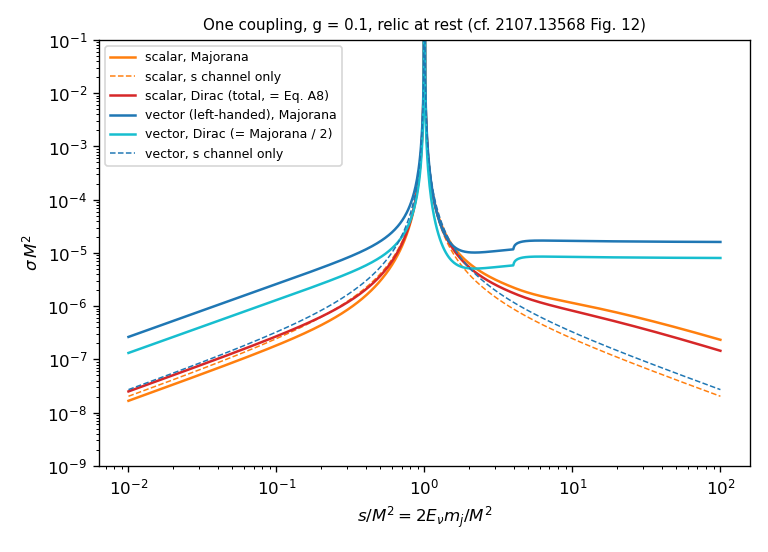
\includegraphics[width=0.62\textwidth]{../output/figures/si_cross_sections_models.png}
\caption{\textbf{Total cross sections} for one coupling, $g = 0.1$, relic at rest: scalar
(Majorana, Dirac) and vector (Majorana; Dirac is half), with the $s$ channels alone. The scalar
Majorana curves reproduce 2107.13568, Fig.~12; all from the closed forms checked by brute force.}
\label{fig:si_xsec}
\end{figure}

\subsection{Transport}
\label{sec:si_transport}

Over cosmological distances the mass states decohere and there is no coherent potential to speak
of (the relic neutrinos' own contribution to the neutrino masses through $\phi$ is negligible), so
the transport follows the number of each mass state per unit observed energy, $F_a(E)$, on the
solver's geometric grid; the physical energy at redshift $z$ is $E(1+z)$, so redshift losses need no
term of their own, and the sources inject $\Phi_0[E(1+z)]^{-p}R(z)\sum_\alpha|U_{\alpha a}|^2f_{\alpha,S}$
per unit time, as for the dark portal. Both helicities of a mass state are followed together: with
real couplings the interaction is CP-symmetric, so their sum evolves exactly whatever the source's
$\bar\nu/\nu$ ratio (the solver returns it split in the injection's proportions; the split of the
secondaries is not modelled).

Redshift steps are uniform in $\ln(1+z)$, one per energy bin by default
(\texttt{z\_substeps}), so that $\mu$ of bin $j$ at the midpoint of step $m$,
$\mu = (M^2/2E_0m_r)\,e^{-(jq + m + 1/2)\Delta}$, falls on one lattice per relic state: the exact
bin integrals of the seven regeneration profiles are tabulated once per mediator and relic masses
(not per coupling, so scans in $g$ reuse them; $\sim30$~MB at the analysis grid). Each step
integrates the optical depth exactly: the Breit--Wigner terms in
$\theta = \arctan[(s - M^2)/M\Gamma]$, in which the resonance is smooth however narrow (a crossing
contributes $\int A(s)\,ds/B = M\Gamma^{-1}\!\int A\,d\theta$, with $A$ the slowly varying density
and Jacobian), the others by Gauss--Legendre in $s$. Then the bins are swept from high to low
energy, each solving its equations over the step exactly with constant rates and sources, and
passing down the number it absorbed: its own secondaries through a $3\times3$ system over the mass
states, those of lower bins through the tabulated profiles. The number at $z = 0$ equals the
injected number plus the secondaries kept in the grid minus the absorbed, to $10^{-14}$. The grid
extends tenfold above $E_{\max}$ so that what is injected above it cascades in. A run takes
$0.3$--$1$~s at the analysis grid (400 bins, 81 steps).

\subsection{Validation}
\label{sec:si_validation}

\begin{table}[h]
\centering
\caption{\textbf{Checks of the secret-interaction module} (\file{tests/test_si.py},
\file{tools/si_validation.py} on Tycho). Deviations of fluxes are relative to the free-streaming
flux at the same energy.}
\label{tab:si_checks}
\small
\begin{tabular}{p{6.6cm}p{7.4cm}}
\toprule
Check & Result \\
\midrule
Channel sums vs Eq.~(A11) as printed; vs quadrature of (A12) + (A13) & $10^{-13}$ (A11 itself loses digits above $s/M^2\sim10^3$) \\
Kinematic integrals vs 50 digits & $4\times10^{-15}$, threshold to $s/M^2 = 10^{14}$ \\
Profile bin integrals vs 30 digits; their sums vs closed-form norms & $1.5\times10^{-14}$; $10^{-14}$, $\mu = 10^{-9}$ to $10^8$ \\
Double-scalar neutrino spectrum vs 30 digits & $2\times10^{-10}$ \\
No coupling vs free streaming & $10^{-14}$ \\
Number balance & $10^{-14}$, every texture, $M$ = 1~keV--1~GeV, $g$ up to 1 \\
Absorption alone vs quadrature of $e^{-\tau}$ along each path & median $10^{-10}$--$7\times10^{-5}$; up to $1.3\%$ in the bins at a narrow resonance's sharp edge (one step per bin; $0.3\%$ with four) \\
Bins and steps vs 1601 bins, four steps per bin (nested grids: no interpolation) & at 401 bins, spectra $1.4\times10^{-3}$ pointwise (median $2.6\times10^{-4}$), up to 3.4\% in the one bin below a very narrow resonance's edge ($g = 0.01$; first order in the bin width); energy-averaged fractions $\le1.2\times10^{-4}$ in all eight cases (scalar and vector, Majorana and Dirac) \\
2107.13568 Fig.~5 & reproduced (Fig.~\ref{fig:si_fig5}) \\
2107.13568 Fig.~3 (Majorana, Dirac) vs their code, nuSIprop & $0.6\%$ above the first dip, $0.2\%$ at the Dirac peak (with the corrected source weighting; Table~\ref{tab:source_checks}) \\
Tree amplitudes by brute force (explicit spinors; Majorana fermions by fermion flow) & (A12), its complex form, the Dirac visible/sterile split $10^{-15}$; vector $|\mathcal M|^2$ $10^{-12}$, longitudinal fraction $3\times10^{-14}$ \\
Vector: tensors vs $\int d\sigma/dt$; narrow $s$ channel vs the Z-burst normalization & $10^{-10}$; $2\times10^{-4}$ \\
Dirac: absorption alone; tracked regeneration over Majorana's & equal to Majorana's (3 digits); $0.499$--$0.500$ \\
Vector far above the resonance vs its closed form (conversions at fixed energy) & flavor fractions $10^{-6}$ \\
Vector drift integrals vs 40 digits; fractions at 201 vs 401 bins (1~keV) & $10^{-7}$; $1.5\times10^{-4}$ ($5\times10^{-3}$ without the drift) \\
\bottomrule
\end{tabular}
\end{table}

The one error above the per-mille level is local and understood: within the step in which a bin
crosses a narrow resonance, the particles injected during the step are treated as exposed to the
step-averaged absorption, while they are in fact absorbed only if injected before the crossing.
It is first order in the step and confined to the one or two bins at the dip's high-energy edge;
energy-averaged fractions do not see it ($10^{-5}$). Splitting the crossing step at the crossing
would remove it, if the event-rate analyses need it.

Figure~\ref{fig:si_fig5} repeats Fig.~5 of 2107.13568 ($\nu_\tau$ couplings, $M = 5$~MeV,
$\nusum = 0.1$~eV in normal ordering, an $E^{-2}$ flux): the two dips at
$\Eres = M^2/2m_j$, the bump of the regenerated neutrinos below them, the slow recovery above the
resonance at $g = 0.1$ (where the $t$ and $u$ channels and double-scalar production dominate), and
the narrow-width approximation that does not depend on $g$ once $g\gtrsim10^{-3}$. At $g = 0.1$,
with their inputs and without double-scalar production (our \texttt{phiphi = "off"}, their default),
our transport agrees with their code, nuSIprop, extrapolated in the bin width, to 1\% from 10~TeV to
10~PeV; at its default 300 bins nuSIprop is still 6--11\% low near the peak (2.09 against 2.35 at
10~TeV), and so is their figure. (Before the correction of App.~\ref{app:source_jacobian} our curve
differed from theirs by up to 35\%, at 100~TeV.)

\begin{figure}[t]
\centering
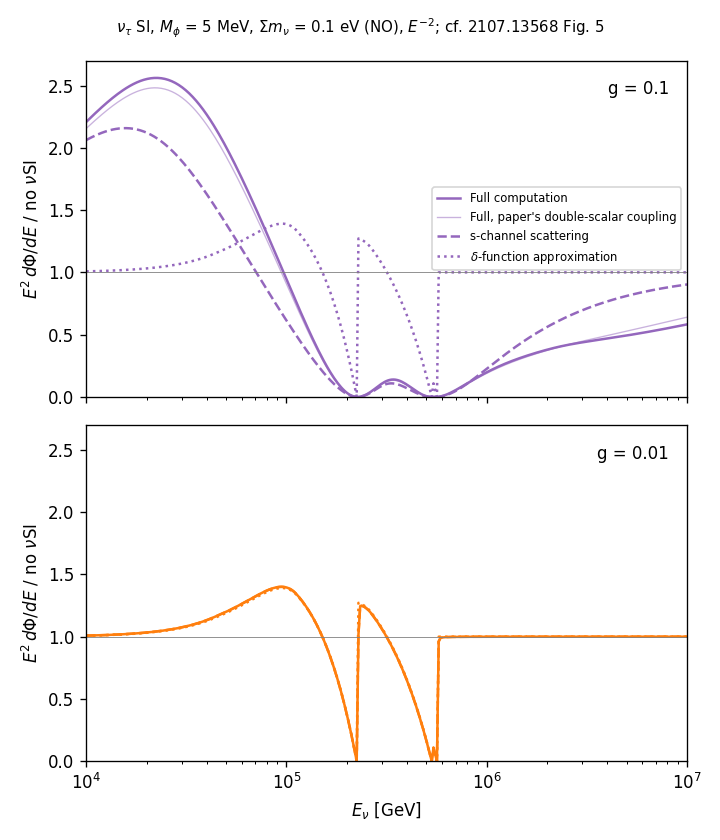
\includegraphics[width=0.62\textwidth]{../output/figures/si_fig5_repro.png}
\caption{\textbf{Fig.~5 of arXiv:2107.13568 recomputed} with \file{src/dp_si.py} (all-flavor flux
over the flux without interactions; $\nu_\tau$ couplings, $M = 5$~MeV, $\nusum = 0.1$~eV in normal
ordering, $E^{-2}$ sources up to $z = 4$; 400 bins). Thin line: the double-scalar coupling as
printed in the paper. \file{tools/si_validation.py}~\texttt{fig5}.}
\label{fig:si_fig5}
\end{figure}

Figure~\ref{fig:si_fig3} repeats the bottom panel of their Fig.~3, the same model at $g = 0.01$
with Majorana and with Dirac neutrinos. With their inputs ($z_{\max} = 5$, $H_0 = 70$, NuFIT~5.0, their
relic density) our transport agrees with their code, nuSIprop, which reproduces their figure: to
$0.6\%$ just above the first dip and $0.2\%$ at the Dirac peak, Majorana and Dirac alike
(Table~\ref{tab:source_checks}). The 9\% difference first found just above the first dip for Dirac
neutrinos came from our sources' redshift weighting, not from the Dirac physics
(App.~\ref{app:source_jacobian}). Our curves also obey two exact relations: absorption alone is the
same for both kinds of neutrino (to three digits at every energy), and with the sterile secondaries
tracked the Dirac regeneration is exactly half the Majorana one ($0.499$--$0.500$ of it at every
energy), as the parity mirror of Sec.~\ref{sec:si_dirac_vector} requires; dropping them, as the paper
does, keeps $0.42$--$0.47$ of it. The source composition plays no role here: with $1:1:1$ (equal mass
states, as theirs) or $1:2:0$ the curves agree to three digits, every state being absorbed in the
dips.

\begin{figure}[t]
\centering
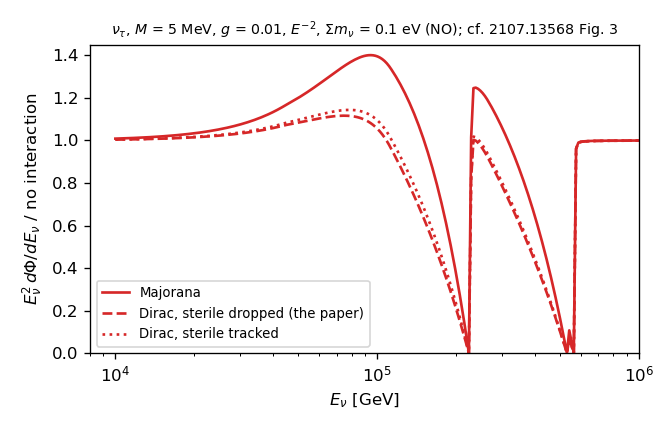
\includegraphics[width=0.6\textwidth]{../output/figures/si_fig3_repro.png}
\caption{\textbf{Fig.~3 (bottom) of arXiv:2107.13568 recomputed}: Majorana neutrinos, and Dirac
neutrinos with the sterile secondaries dropped (as the paper does) or tracked; $\nu_\tau$
couplings, $M = 5$~MeV, $g = 0.01$, otherwise as Fig.~\ref{fig:si_fig5}.
\file{tools/si_validation.py}~\texttt{fig3}, \file{tools/plot_si_summary.py}~\texttt{fig3}.}
\label{fig:si_fig3}
\end{figure}

\subsection{The flavor-triangle planes}
\label{sec:si_planes}

We ran the flavor-triangle analysis of Sec.~\ref{sec:stats} with the secret interactions in place
of the dark portal: the projected 2050 measurement for pion sources, the projection's mixing,
$m_{\rm lightest} = 0.01$~eV, $E^{-2.5}$ sources up to $z = 4$, the whole sky (no Earth effect
here), and planes in $(M, g)$ for four textures, $\nu_e$, $\nu_\mu$ or $\nu_\tau$ couplings alone
and flavor-universal ones, and three non-universal textures of two flavors, $g$ on $\nu_e$ and
$\nu_\mu$, $\nu_e$ and $\nu_\tau$, or $\nu_\mu$ and $\nu_\tau$ ($49\times49$ points from 1~keV to
1~GeV and $g = 10^{-6}$ to 1, read per mass at $\Delta\chi^2 = 3.84$; Tycho, commits
\texttt{fe8e2dc} for the single flavors and \texttt{a6570a6}, with the couplings $U^TGU$, for the
others; 4--9 minutes each on 16 cores; configurations \file{pion_2050_case_5_si_*.json}). Every mass column reaches the region without an
effect: $\Delta\chi^2 = 0.00$ at $g = 10^{-6}$ (a first run starting at $g = 10^{-4}$ did not, near
1~MeV). Figure~\ref{fig:si_planes} shows the planes and Fig.~\ref{fig:si_paths} how the composition
moves.

The limits have three regimes. Below $\sim200$~keV every resonance lies below the band and the
non-resonant channels act alone, with $\sigma\sim g^4/8\pi s$ independent of $M$: the limit is
flat, $g < 5.8\times10^{-3}$--$8.2\times10^{-3}$ ($\nu_e$), $6.9\times10^{-3}$--$1.1\times10^{-2}$
($\nu_\mu$, $\nu_\tau$), $4.5\times10^{-3}$--$8\times10^{-3}$ (universal), $5\times10^{-3}$--$10^{-2}$
for the pairs with $\nu_e$. Between $\sim0.5$ and 3~MeV the
resonances $\Eres = M^2/2m_j$ fall at 10--50~TeV, at the bottom of the band, where the $E^{-2.5}$
flux dominates the energy-averaged fractions, and the limits drop by two to three decades:
$g < 1.5\times10^{-5}$ ($\nu_e$, at 0.56~MeV), $2.9\times10^{-5}$ ($\nu_\mu$, 0.56~MeV),
$8.3\times10^{-5}$ ($\nu_\tau$, 0.75~MeV), $8.0\times10^{-6}$ (universal, 0.56~MeV), and
$1.3\times10^{-5}$, $1.0\times10^{-5}$, $1.7\times10^{-5}$ for the pairs $e\mu$, $e\tau$, $\mu\tau$.
Above, the resonances move above most of the flux and the limits weaken: at 10~MeV $g < 0.13$,
$0.27$, $0.30$, $0.064$ and $0.086$, $0.073$, $0.12$; above 30~MeV only the universal coupling and the
pairs with $\nu_e$ are still limited ($g < 0.75$, $0.98$ and $0.81$ at 100~MeV).

Two features follow from flavor fractions being the only observable. Flavor-blind absorption does
not change the composition: universal couplings act on it through the mass-dependent resonance
energies and through the off-diagonal couplings of $g\,U^TU$. With $g\,\mathbb{1}$, as the paper
would have it, the effects of the $m_3$ and the $m_{1,2}$ resonances compensated near 1~MeV and left
an allowed gap ($g < 10^{-2}$ there, as the couplings diagonal in the mass basis of
Sec.~\ref{sec:si_models} still show); the off-diagonal couplings close most of it
($1.7\times10^{-4}$ at 1~MeV). And as $g$ grows the
composition can pass back through the projection's centre: thin allowed islands and channels run
through the excluded regions (the widest, for the $\mu\tau$ pair near 100~keV, raises the limit read
there to $0.09$; Fig.~\ref{fig:si_paths} shows the paths, nearly straight lines through the standard
point). Spectral data will remove both;
they will also exclude much of the plane outright, since at $g\gtrsim10^{-2}$ below 1~MeV more than
99\% of the flux below $10^7$~GeV is absorbed, which normalized fractions do not see. The resonant
window overlaps the region below $\sim2$~MeV that Big-Bang nucleosynthesis already disfavors
(2107.13568, Fig.~1).

\begin{figure}[t]
\centering
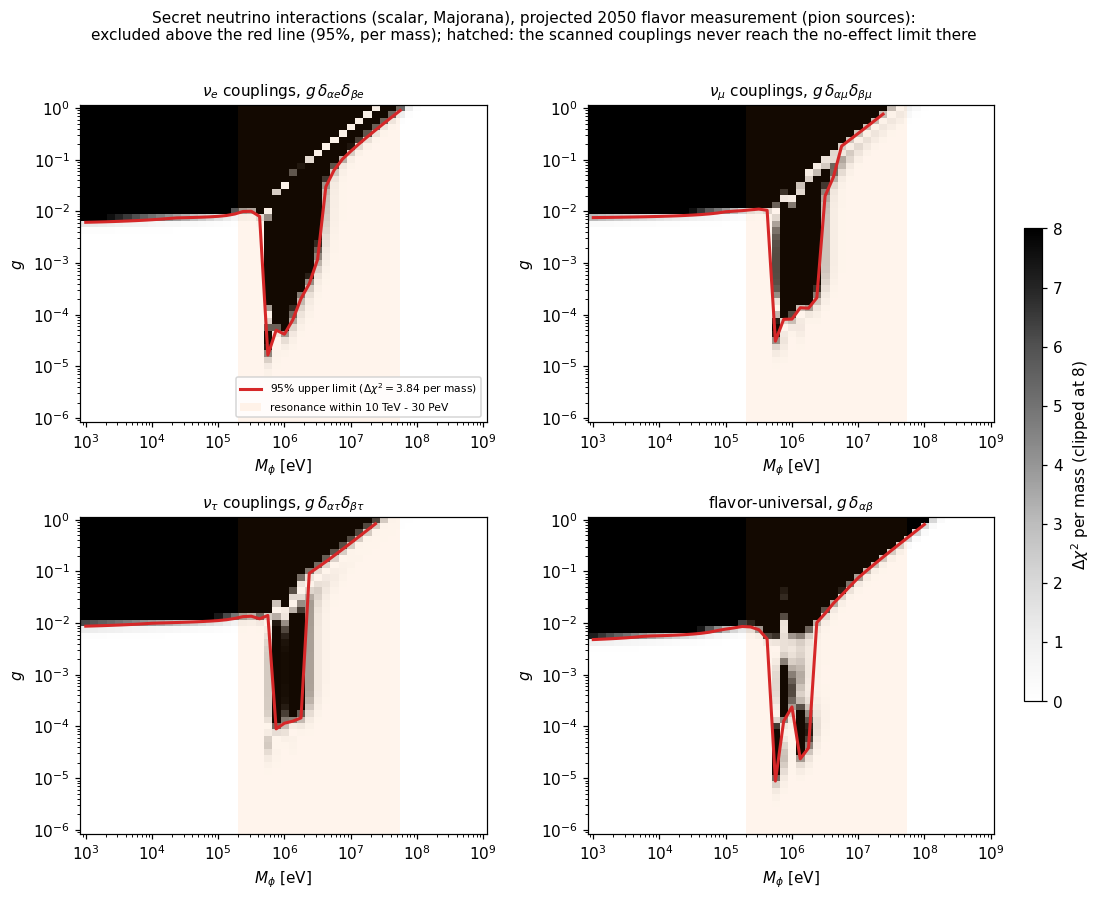
\includegraphics[width=\textwidth]{../output/figures/si_planes_summary.png}
\caption{\textbf{Secret-interaction exclusion planes} of the projected 2050 flavor measurement
(pion sources; scalar mediator, Majorana neutrinos): $\Delta\chi^2$ per mediator mass and the 95\%
upper limit (red; the top of each column's lowest allowed interval). Shaded: masses whose resonance
falls in 10~TeV--30~PeV for some $z\le4$. \file{tools/plot_si_summary.py}~\texttt{planes}.}
\label{fig:si_planes}
\end{figure}

\begin{figure}[t]
\centering
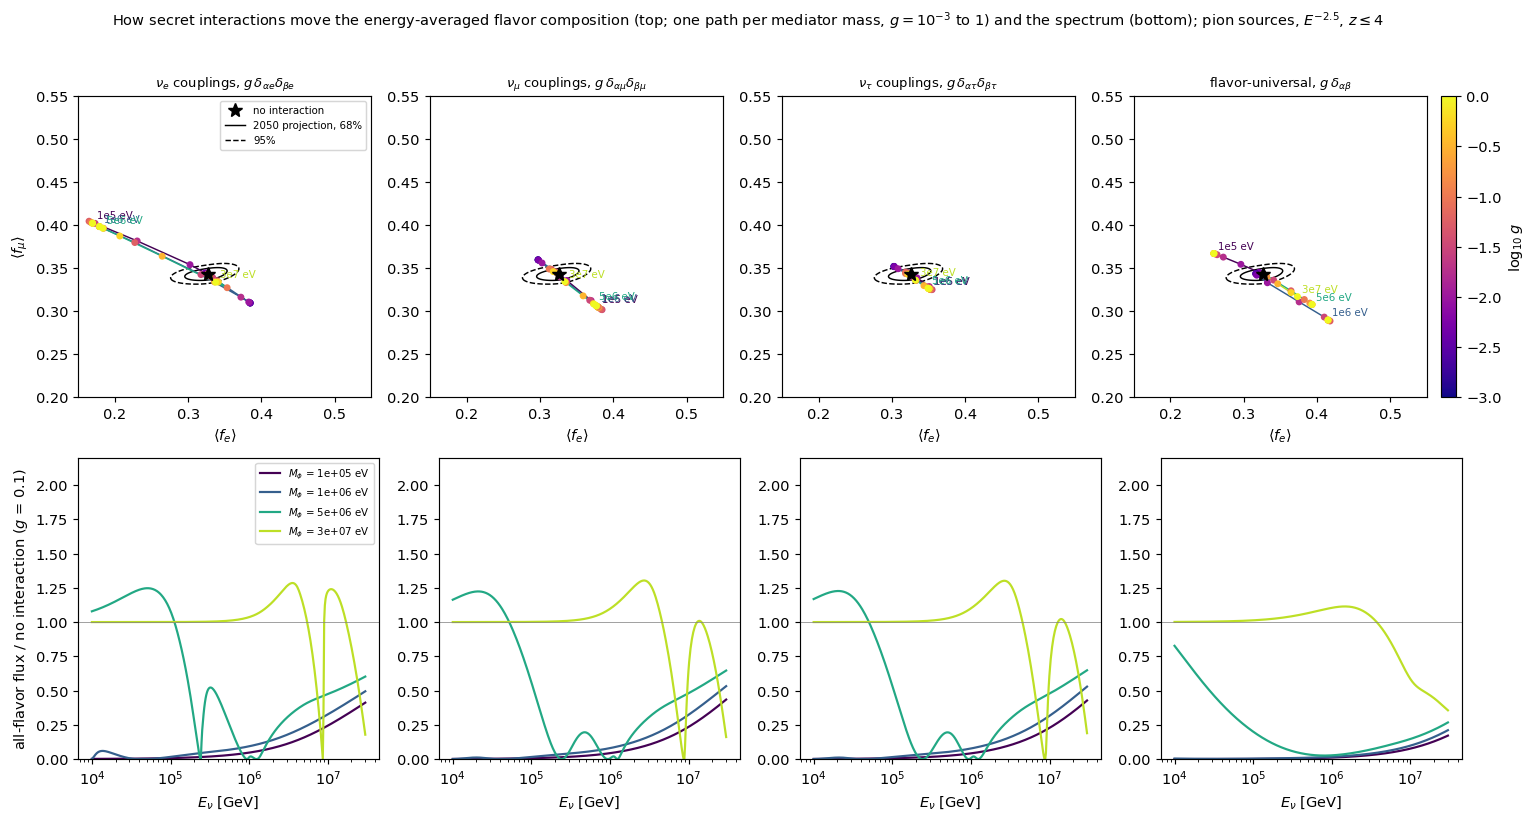
\includegraphics[width=\textwidth]{../output/figures/si_flavor_paths.png}
\caption{\textbf{How the composition moves.} Top: energy-averaged $(f_e, f_\mu)$ at the detector as
$g$ goes from $10^{-3}$ to 1 at four mediator masses, against the projection's 68\% and 95\%
contours. Bottom: the all-flavor flux at $g = 0.1$ over the flux without interactions.
\file{tools/si_flavor_paths.py} (Tycho), \file{tools/plot_si_summary.py}~\texttt{paths}.}
\label{fig:si_paths}
\end{figure}

\begin{figure}[t]
\centering
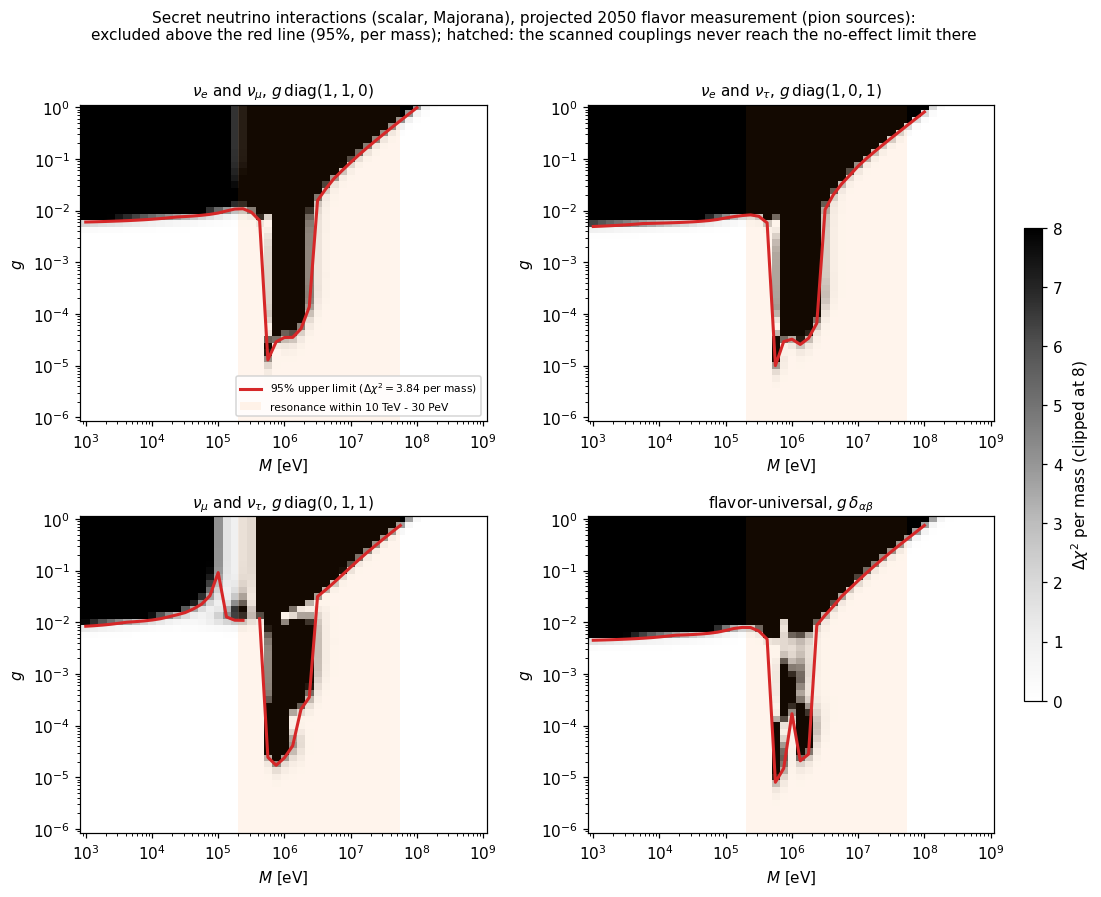
\includegraphics[width=\textwidth]{../output/figures/si_planes_two_flavor.png}
\caption{\textbf{Non-universal textures of two flavors}, as Fig.~\ref{fig:si_planes}: $g$ on
$\nu_e$ and $\nu_\mu$, $\nu_e$ and $\nu_\tau$, $\nu_\mu$ and $\nu_\tau$ (complex mass-basis couplings
$U^TGU$ at $\delta_{CP} = 212^\circ$), and the universal coupling again.
\file{tools/plot_si_summary.py}~\texttt{planes2}.}
\label{fig:si_planes2}
\end{figure}

\subsection{Four models}
\label{sec:si_models}

We repeated the four planes of Fig.~\ref{fig:si_planes} for the scalar with Dirac neutrinos and for
the vector with Majorana and with Dirac neutrinos (configurations
\file{pion_2050_case_5_si_{dirac,vector,vector_dirac}_*.json}, the same grid; Tycho jobs
66307194--97 (commit \texttt{124fd03}, with the drift and the corrected source weighting of
App.~\ref{app:source_jacobian}); 7--13 minutes per plane on 16 cores, the Dirac scalar the slowest, with two transport runs per point; the vector
Dirac planes are in \file{output/figures/si_planes_vector_dirac.png}). Figure~\ref{fig:si_models_spectra} shows one benchmark
under the four models, Fig.~\ref{fig:si_limits} and Table~\ref{tab:si_limits} the limits, and
Figs.~\ref{fig:si_planes_vector} and \ref{fig:si_planes_dirac} two of the models' planes.

\textit{The resonant window} (0.5--3~MeV) gives the strongest limits in all four, within a factor
$\sim1.5$ of each other at its best mass (absorption alone being the same for Majorana and Dirac
neutrinos, Sec.~\ref{sec:si_validation}). For the Dirac scalar the excluded region inside the
window breaks into islands (Fig.~\ref{fig:si_planes_dirac}), where the composition's path passes back
through the projection's centre, as it does more rarely for Majorana neutrinos
(Sec.~\ref{sec:si_planes}); the per-mass reading then jumps with the channels: for $\nu_\tau$ at
0.56~MeV it is $5.6\times10^{-5}$ for Dirac neutrinos, while an allowed channel lifts the Majorana
reading to $1.4\times10^{-2}$; at 0.75~MeV, $1.8\times10^{-4}$ against $8.3\times10^{-5}$.
Fine scans of these columns (121 couplings, with the planes' own objective; Fig.~\ref{fig:si_islands})
reproduce the planes' points exactly and their readings within one grid step, so the channels are
resolved and real: along a column $\Delta\chi^2$ falls back to $\simeq0$ wherever the composition's
path crosses the projection's centre. They also show what the single line hides: at 0.56~MeV the
Dirac column crosses 3.84 only in a narrow peak near $g\simeq6\times10^{-5}$ and stays allowed
($\Delta\chi^2\simeq0.5$) from $10^{-4}$ to $10^{-2}$; the planes' shading shows it, the per-mass
reading of the lowest allowed interval does not.

\begin{figure}[t]
\centering
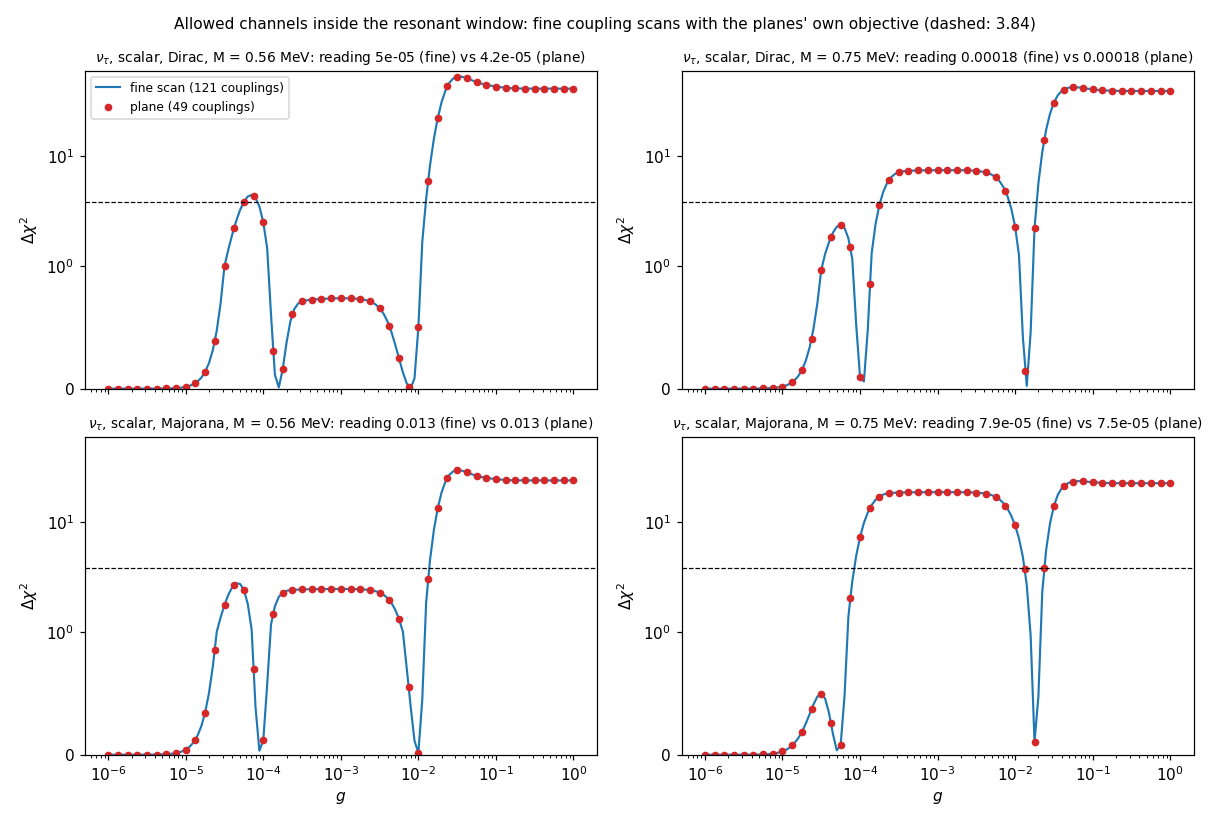
\includegraphics[width=\textwidth]{../output/figures/si_island_check.png}
\caption{\textbf{Allowed channels inside the resonant window}: $\Delta\chi^2$ along four mass columns of
the $\nu_\tau$ planes (scalar, Majorana and Dirac, $M = 0.56$ and $0.75$~MeV), fine scans of 121
couplings with the planes' objective (line) against the planes' 49 points (dots); dashed: 3.84.}
\label{fig:si_islands}
\end{figure}

\textit{Below the window} the vector's quasi-elastic conversions (Sec.~\ref{sec:si_dirac_vector})
set the limit for the single-flavor textures, $g\propto\sqrt M$: $4.4\times10^{-4}$ for $\nu_e$ at
1~keV, thirteen times below the scalar's $5.8\times10^{-3}$, with the flux intact. Their effect
saturates at equal mass states, and where that shift is no longer enough (20--50~keV for $\nu_e$)
the limit comes from hard scatterings, as for the scalar. Flavor-universal couplings stay diagonal in
the mass basis for the vector and for the Dirac scalar, $U^\dagger(g\mathbb 1)U = g\mathbb 1$: no
conversions, and the 1-MeV gap of $g\mathbb 1$ that $U^TU$ closes for the Majorana scalar
(Sec.~\ref{sec:si_planes}) remains for all three ($g < 0.010$--$0.011$ there, against
$1.7\times10^{-4}$). Below 400~keV universal vector couplings are not limited at all: the energy loss
of their forward-peaked scatterings can remove the whole flux from the band (to $2\times10^{-4}$ of
its number at 1~keV and $g = 0.03$) while hardly moving its composition ($f_e$ by $-0.016$,
$\Delta\chi^2 < 3.84$), which normalized fractions cannot see. Spectral data will exclude that region
outright. (Before the drift of Sec.~\ref{sec:si_dirac_vector}, it appeared excluded above
$g\simeq4\times10^{-3}$: an artifact of the missing energy loss.)

\textit{Above the window} the vector is limited further, because its cross section stays constant
above the resonance where the scalar's falls as $1/s$: $g < 0.071$ for $\nu_e$ at 10~MeV (scalar
$0.13$), and for $\nu_e$ a limit up to 100~MeV ($0.74$). Dirac rates of the vector are half the Majorana ones, and its
limits are weaker by $2^{1/4}\simeq1.2$ wherever one process dominates (1~keV: $5.2\times10^{-4}$
against $4.4\times10^{-4}$ for $\nu_e$).

\begin{table}[h]
\centering
\caption{\textbf{95\% upper limits on $g$ of the four models} (projected 2050 flavor measurement,
pion sources; per mass at $\Delta\chi^2 = 3.84$, the top of each column's lowest allowed interval).
S/V: scalar/vector; M/D: Majorana/Dirac; best: the strongest limit and its mass in MeV; --: no limit
up to $g = 1$ (or the column never reaches the no-effect limit). \file{output/analysis/}.}
\label{tab:si_limits}
\small
\begin{tabular}{llccccc}
\toprule
Texture & Model & Best (MeV) & 1~keV & 100~keV & 10~MeV & 100~MeV \\
\midrule
$\nu_e$    & S, M & $1.5\times10^{-5}$ (0.56) & $5.8\times10^{-3}$ & $7.7\times10^{-3}$ & 0.13 & -- \\
           & S, D & $1.8\times10^{-5}$ (0.56) & $5.7\times10^{-3}$ & $7.0\times10^{-3}$ & 0.2 & -- \\
           & V, M & $1.2\times10^{-5}$ (0.56) & $4.4\times10^{-4}$ & $5.7\times10^{-3}$ & 0.071 & 0.74 \\
           & V, D & $1.7\times10^{-5}$ (0.56) & $5.2\times10^{-4}$ & $6.6\times10^{-3}$ & 0.084 & 0.85 \\
\midrule
$\nu_\mu$  & S, M & $2.9\times10^{-5}$ (0.56) & $6.9\times10^{-3}$ & $8.7\times10^{-3}$ & 0.27 & -- \\
           & S, D & $3.2\times10^{-5}$ (0.75) & $7.0\times10^{-3}$ & $8.4\times10^{-3}$ & 0.15 & -- \\
           & V, M & $2.2\times10^{-5}$ (0.56) & $8.1\times10^{-4}$ & $4.7\times10^{-3}$ & 0.14 & -- \\
           & V, D & $3.1\times10^{-5}$ (0.56) & $9.5\times10^{-4}$ & $5.7\times10^{-3}$ & 0.17 & -- \\
\midrule
$\nu_\tau$ & S, M & $8.3\times10^{-5}$ (0.75) & $8.1\times10^{-3}$ & 0.011 & 0.3 & -- \\
           & S, D & $5.6\times10^{-5}$ (0.56) & $8.0\times10^{-3}$ & 0.01 & 0.18 & -- \\
           & V, M & $5.8\times10^{-5}$ (0.75) & $7.2\times10^{-4}$ & $5.3\times10^{-3}$ & 0.15 & -- \\
           & V, D & $8.1\times10^{-5}$ (0.75) & $8.7\times10^{-4}$ & $6.4\times10^{-3}$ & 0.18 & -- \\
\midrule
universal  & S, M & $8.0\times10^{-6}$ (0.56) & $4.5\times10^{-3}$ & $7.0\times10^{-3}$ & 0.064 & 0.75 \\
           & S, D & $1.1\times10^{-5}$ (0.56) & $5.2\times10^{-3}$ & $7.3\times10^{-3}$ & 0.065 & 0.75 \\
           & V, M & $5.7\times10^{-6}$ (0.56) & -- & -- & -- & -- \\
           & V, D & $7.9\times10^{-6}$ (0.56) & -- & -- & -- & -- \\
\bottomrule
\end{tabular}
\end{table}

\begin{figure}[t]
\centering
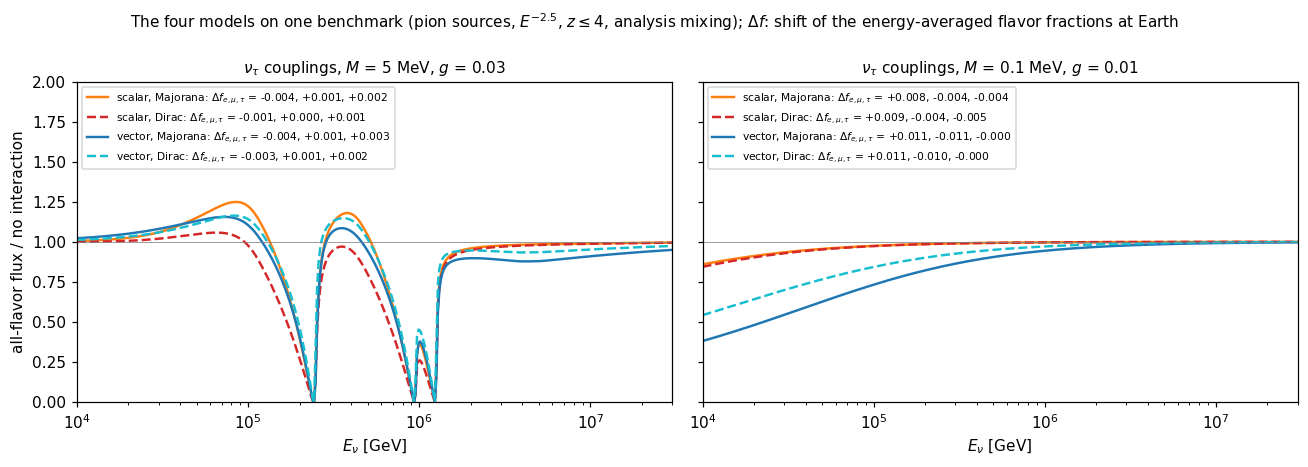
\includegraphics[width=\textwidth]{../output/figures/si_models_spectra.png}
\caption{\textbf{One benchmark under the four models}: all-flavor flux over the flux without
interactions, $\nu_\tau$ couplings, and the shift of the energy-averaged flavor fractions at Earth.
Left: $M = 5$~MeV, $g = 0.03$ (the resonant dips; above them the vector's constant cross section
keeps acting). Right: $M = 0.1$~MeV, $g = 0.01$ (resonances below the band: the scalar's
non-resonant channels against the vector's forward peak). \file{tools/si_validation.py}~\texttt{models},
\file{tools/plot_si_summary.py}~\texttt{models}.}
\label{fig:si_models_spectra}
\end{figure}

\begin{figure}[t]
\centering
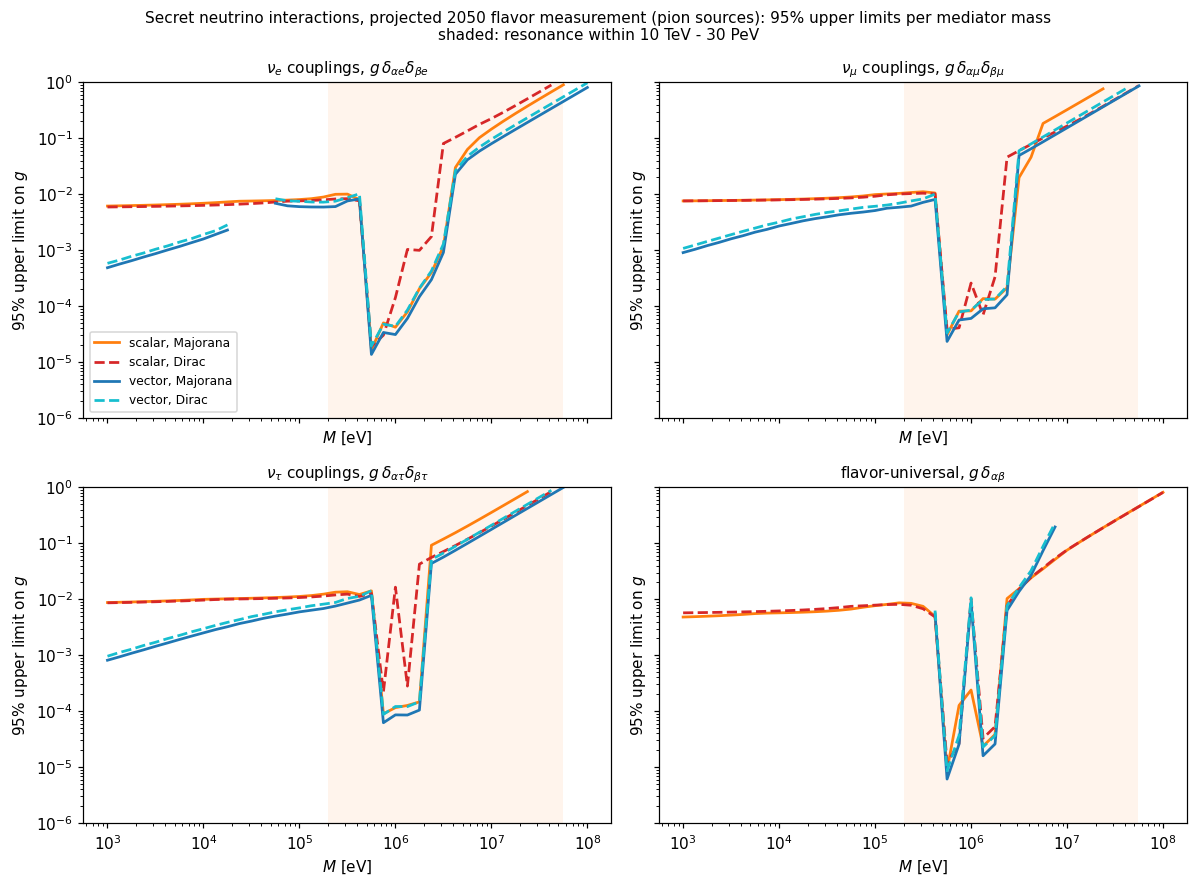
\includegraphics[width=\textwidth]{../output/figures/si_limits_models.png}
\caption{\textbf{95\% upper limits of the four models} per mediator mass and texture (as
Fig.~\ref{fig:si_planes}). Gaps: masses with no limit up to $g = 1$, or whose lowest allowed
interval is open. \file{tools/plot_si_summary.py}~\texttt{limits}.}
\label{fig:si_limits}
\end{figure}

\begin{figure}[t]
\centering
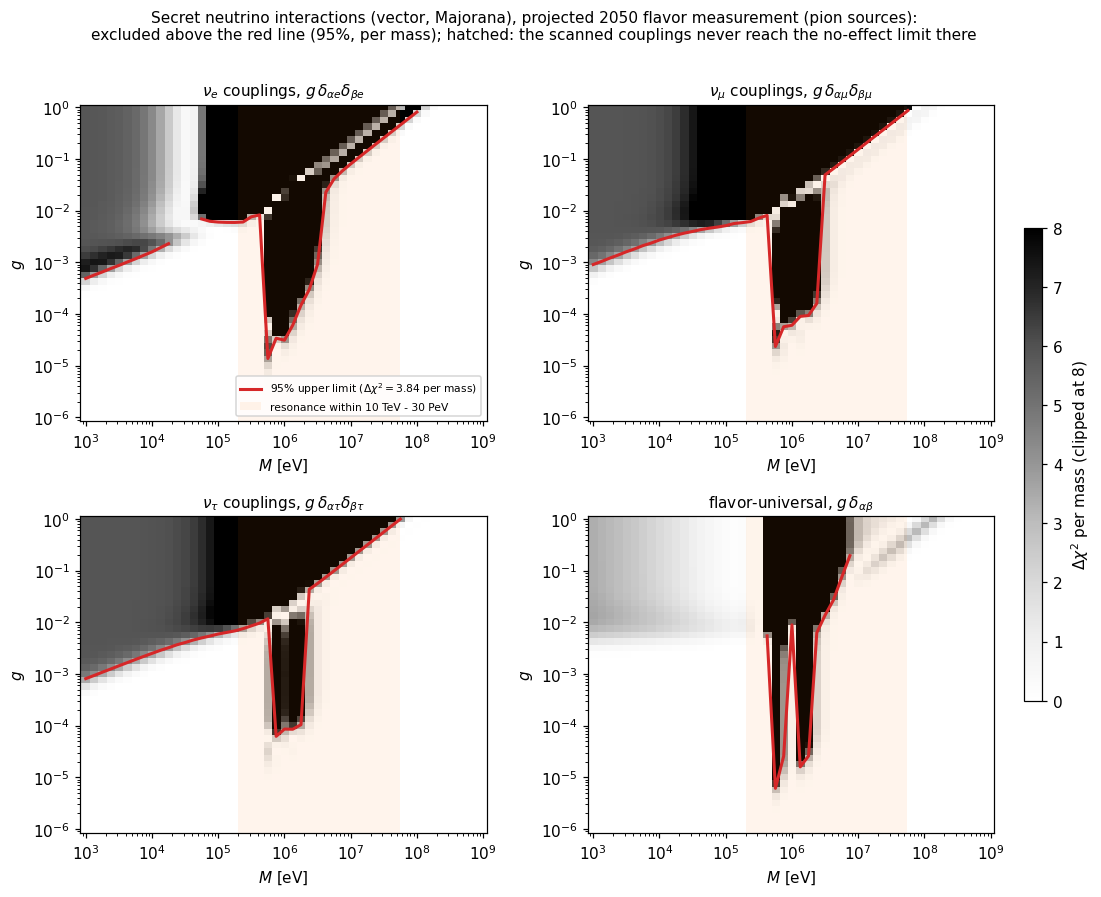
\includegraphics[width=\textwidth]{../output/figures/si_planes_vector.png}
\caption{\textbf{Exclusion planes of the vector mediator} (Majorana neutrinos), as
Fig.~\ref{fig:si_planes}. Below the window, the quasi-elastic conversions ($g\propto\sqrt M$) for
single flavors. \file{tools/plot_si_summary.py}~\texttt{planes}, tag \texttt{vector\_}.}
\label{fig:si_planes_vector}
\end{figure}

\begin{figure}[t]
\centering
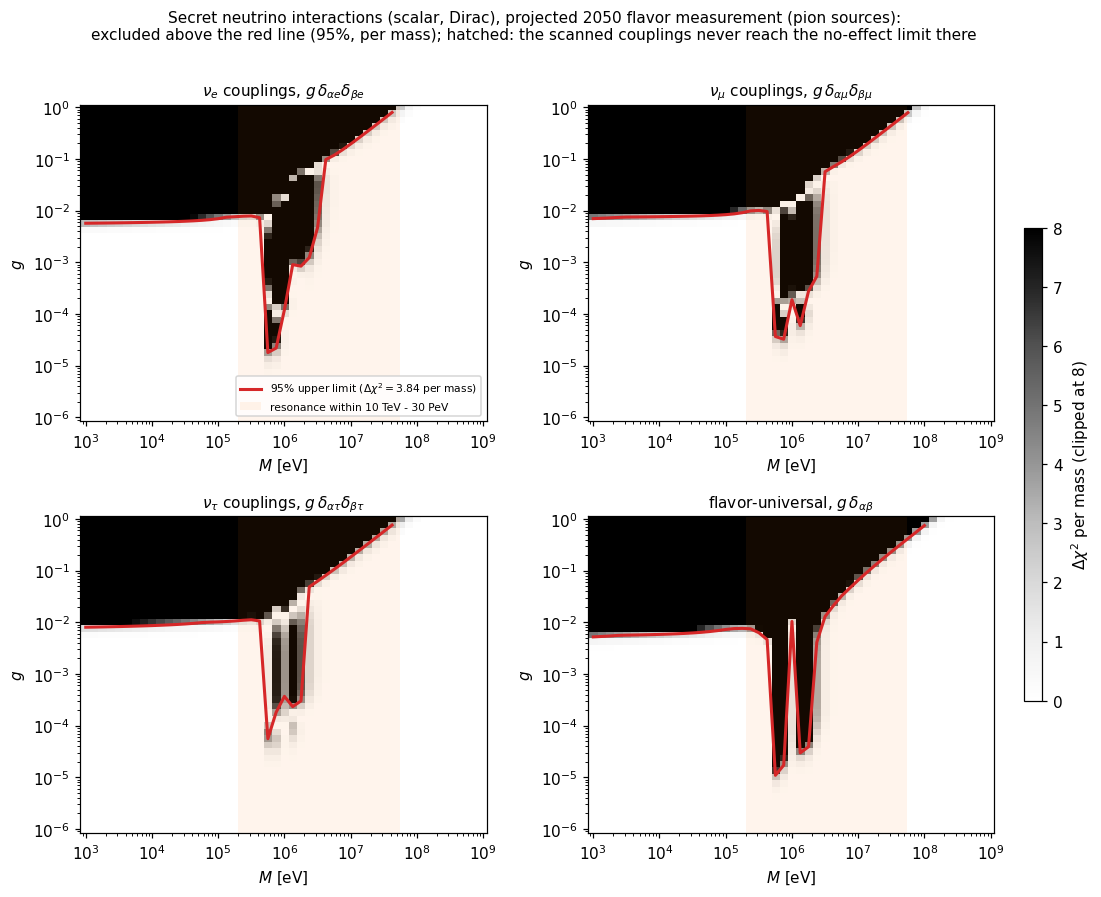
\includegraphics[width=\textwidth]{../output/figures/si_planes_dirac.png}
\caption{\textbf{Exclusion planes of the scalar with Dirac neutrinos} (sterile secondaries
tracked), as Fig.~\ref{fig:si_planes}: inside the resonant window the excluded region breaks into
islands. \file{tools/plot_si_summary.py}~\texttt{planes}, tag \texttt{dirac\_}.}
\label{fig:si_planes_dirac}
\end{figure}

\textit{Not yet included.}---The relic neutrinos' thermal momenta (relics are at rest here, as in
both papers; this matters for a nearly massless lightest state, whose relics are relativistic), the
timing within the crossing step (Sec.~\ref{sec:si_validation}), and spectral data, which would
exclude outright the regions where the flux is absorbed without changing its composition.


%==============================================================================
\section{Arrival directions and Galactic sources}
\label{sec:directions}

On 2026-10-13 Mauricio asked for per-direction output and a Galactic-source component, with an
implementation plan backed by published work before any code. The plan
(\file{docs/dev/DIRECTIONS_PLAN.md}, decisions D1--D6) was written from surveys of the solver's
direction handling, the literature on Galactic diffuse neutrinos and on new physics with directions,
and the sibling projects' data. This section collects its results as they land.

\textit{Sky and frames.}---\file{src/dp_sky.py}: HEALPix pixels in RING ordering (Gorski et al.\
2005), equatorial J2000 with the IAU 1958 Galactic frame in its FK5 realization (agreeing with astropy
to $7\times10^{-10}$~rad), the ecliptic, and the zenith at the South Pole, $\cos\theta_z = -\sin\delta$
at every time, so that the Earth's part of the flux depends on declination only. Output in 20
declination bands of equal solid angle (0.1 in $\sin\delta$) and HEALPix maps at $N_{\rm side} = 16$
(decision D1).

\textit{The Earth per band.}---The phase-aware zenith average restricted to each band
(App.~\ref{app:zenith}, last paragraph): the bands weighted by solid angle return the whole sky to
rounding, and each band matches the exact integral over its range. \file{propagate_sky} returns the
bands for neutrinos and antineutrinos separately; secret interactions are isotropic.

\textit{The Sun per direction (decision D4: measure first).}---Over a year a direction at ecliptic
latitude $\beta$ sees the Sun at $\cos\psi = \cos\beta\cos(\lambda - \lambda_\odot(t))$ (Kepler orbit);
its flux is $\sum_p a_p F_p$ over the transit's Gauss--Legendre paths, with $a_p$ the year-average of
the Lagrange basis on the path cosines, which averages over the sky to the Gauss--Legendre weights
(isotropy recovered exactly; the path runs recombine to the isotropic one to rounding). At twelve
points across the Sun's window ($\mzd = 10^{-24}$ to $10^{-18}$~eV; the Sun's potential at the Earth
0.3, 1 and 3 times $\Delta m^2_{31}/(2\times100$~TeV$)$, $e\mu$ texture) the yearly per-direction
weighting moves the energy-averaged flavor fractions of a pixel by at most $1.2\times10^{-3}$, and by
$10^{-5}$--$5\times10^{-4}$ typically, against $6.4\times10^{-3}$ for single paths: every direction
sweeps through angles to the Sun over the year (Fig.~\ref{fig:sun_aniso}). The effect falls as the
Sun's potential grows, where its crossing becomes adiabatic and depends only on the endpoints (as
found for supernova neutrinos, arXiv:2607.24918). The Sun is kept isotropic;
\file{tools/sun_anisotropy.py}.

\begin{figure}[t]
\centering
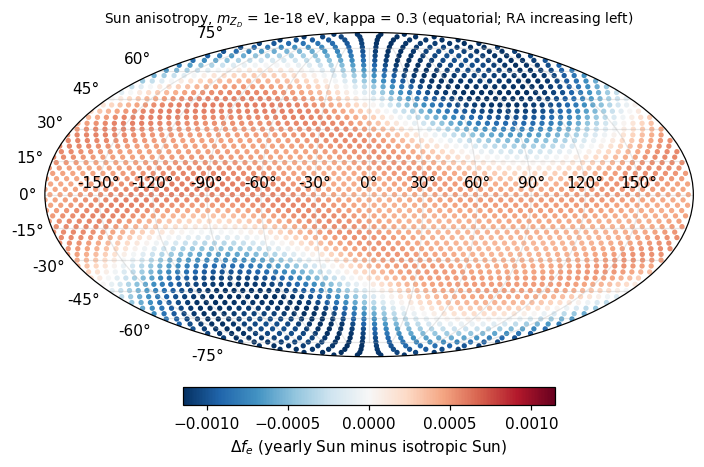
\includegraphics[width=0.7\textwidth]{../output/figures/sun_anisotropy.png}
\caption{\textbf{The Sun's anisotropy} at its largest among the points scanned ($\mzd = 10^{-18}$~eV,
the Sun's potential 0.3 times the vacuum term at 100~TeV): the energy-averaged $\nu_e$ fraction with
the yearly per-direction weighting minus the isotropic Sun average, per HEALPix pixel ($N_{\rm side} =
16$, equatorial). The pattern follows the ecliptic.}
\label{fig:sun_aniso}
\end{figure}

\textit{The Galactic templates (decision D2).}---Two templates, each in IceCube's convention (per
flavor, $\nu+\bar\nu$; the release README of doi:10.21234/8v5d-rn16) and reduced on Tycho to
equatorial $N_{\rm side} = 16$ maps from 72~GeV to $10^8$~GeV (\file{tools/prepare_galactic.py}):
CRINGE (Schwefer, Mertsch \& Wiebusch 2023, Zenodo 7859442) and the Fermi-LAT $\pi^0$ template with
$E^{-2.7}$, whose model flux is $E^2\Phi(100~{\rm TeV}) = 4.4\times10^{-12}$~TeV~cm$^{-2}$~s$^{-1}$,
sky-integrated per flavor (arXiv:2607.25966, supplement). The frames are read off the maps (CRINGE is
Galactic, IceCube's $\pi^0$ map equatorial; toise's Galactic copy of the latter, rotated by our code,
correlates with it at 0.997). The test is IceCube's own fit: times its 2026 normalizations (0.91 for
CRINGE, 4.99 for $\pi^0$) our inner-Galaxy spectra ($|b| < 15^\circ$, $|l| < 20^\circ$) lie on the curves
of arXiv:2607.25966 Fig.~4, read from the figure's SVG path coordinates, to 0.25\% and 0.47\%
(Fig.~\ref{fig:galactic_templates}). That test exposed what IceCube calls CRINGE: the diffuse map
\emph{plus} CRINGE's unresolved-source map. The diffuse map alone reaches only 28--54\% of the fitted
curve, and is softer; the unresolved sources carry 75\% of the sky-integrated flux at 100~TeV and
dominate the inner Galaxy above $\sim$30~TeV. For the dark portal's emission points (plan step 6) this
makes the source distribution, not the gas, the main term above 30~TeV.

\textit{The Galactic component.}---We keep each template's all-flavor total and apply our own physics
(\file{src/dp_galactic.py}): sources of composition $(x, 1-x, 0)$ (decision D6, $x$ floated on its
own; $1/3$ for pion decay), $\nu:\bar\nu = 1:1$. Under secret interactions the Galactic flux is
unattenuated (the Galactic relic column is $\sim$$10^{-5}$ of the cosmological one) with oscillations
averaged over kiloparsecs. For the dark portal, emission at the local potential (option \texttt{local}; the
3-D emission points below are the default): the flavors decohere into the local eigenstates, populations $\sum_\alpha
f_\alpha|W_{\alpha k}|^2$, and from there cross the Sun and the Earth as the extragalactic flux does, per
declination band. \file{propagate_sky} returns the component in physical units next to the extragalactic
one. Checks (\file{tests/test_galactic.py}): the transfer conserves the flux to $3\times10^{-14}$ and is
linear in $x$; without the dark potential it is the averaged oscillation to $10^{-12}$; with the Earth's
standard matter potential on, the bands through the Earth move by the MSW effect on the arriving
mass-state mixture, $2.4\times10^{-5}$ at 10~TeV through the core and falling as $1/E$.

\begin{figure}[t]
\centering
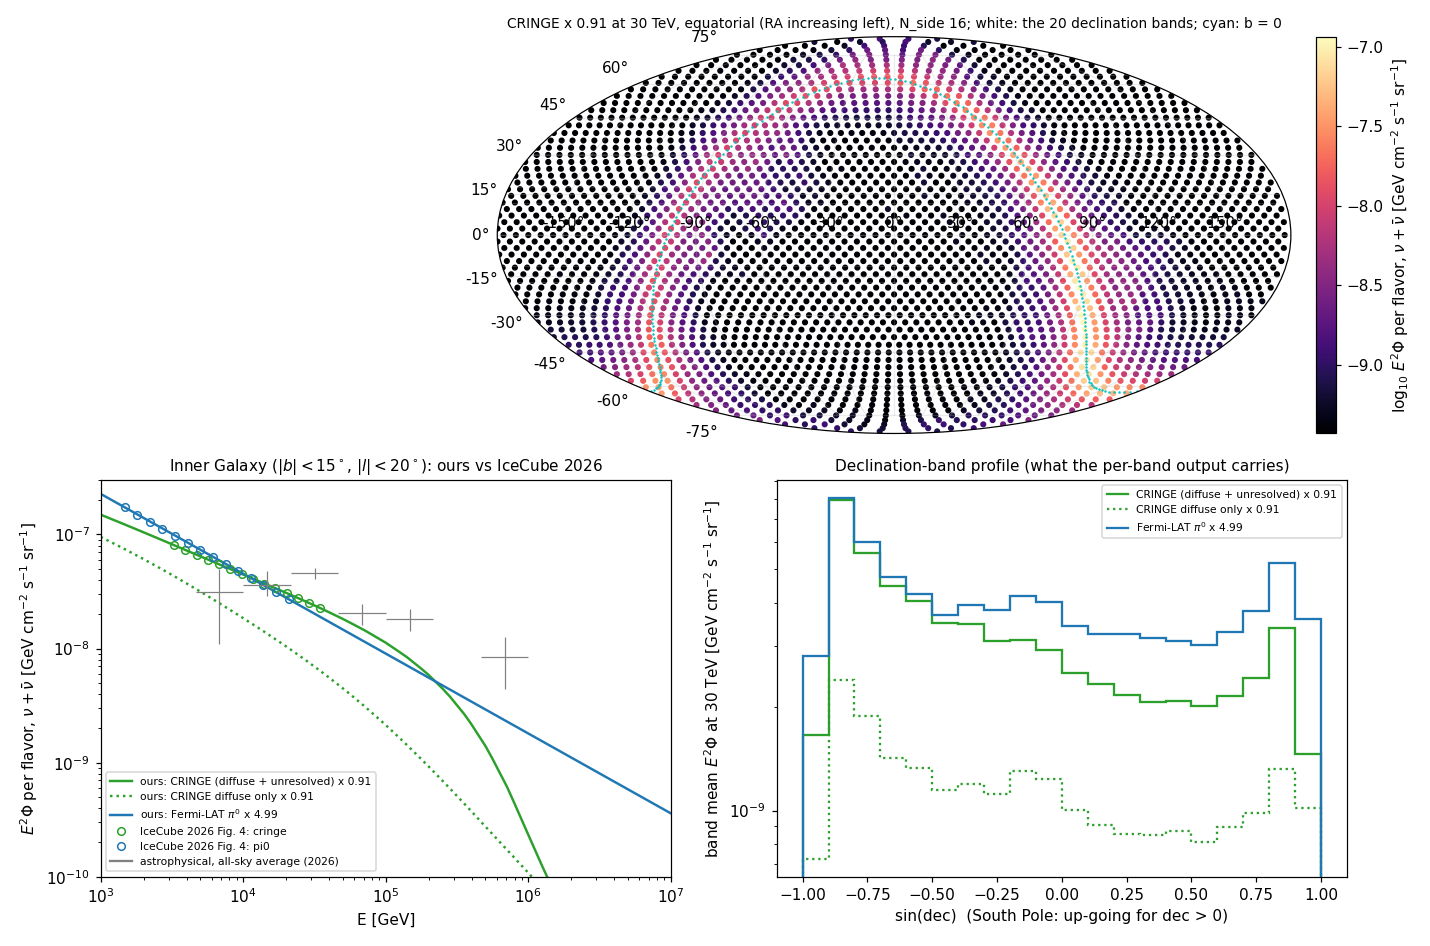
\includegraphics[width=\textwidth]{../output/figures/galactic_templates.png}
\caption{\textbf{The Galactic templates.} Top: CRINGE (diffuse plus unresolved sources) times 0.91 at
30~TeV, equatorial, with the 20 declination bands. Bottom left: inner-Galaxy spectra, ours (lines)
against IceCube's 2026 best fits (circles, arXiv:2607.25966 Fig.~4) and its all-sky astrophysical flux
(grey); the dotted line is CRINGE's diffuse map alone. Bottom right: the band means the per-band output
carries.}
\label{fig:galactic_templates}
\end{figure}

\textit{Emission points in three dimensions (decision D3).}---For the dark portal, a Galactic neutrino is
born in the eigenstates of the potential at its emission point and, the Galaxy's potential changing over
$\gtrsim 10$~pc against oscillation lengths $\lesssim 10^{-3}$~pc, keeps their populations on its way to the
Sun. The potential there is the Yukawa-smoothed neutron density $n_{\rm eff}(\vec x; m)$, now tabulated at any
point of the Galaxy (\file{tools/mw_neff_tables.py}): sphere averages of our Galactic model around $48\times22$
nodes in $(R, z)$, integrated on the solver's own distance nodes, for 20 masses per decade from $10^{-34}$ to
$10^{-12}$~eV. At the Sun's node it equals the solver's local potential to $10^{-9}$ (test T7). Far beyond the
Galaxy's size $n_{\rm eff}$ is \emph{not} uniform: the Galaxy's share is $m^2$ times its neutrons'
``Coulomb'' potential at the point, about six times deeper at the Centre than at the Sun, and it exceeds the
cosmic floor down to $\sim4\times10^{-31}$~eV; only beyond the Hubble radius is the pattern frozen.
Where along each line of sight the neutrinos are born follows the two components of CRINGE: the gas (hydrogen
columns of S\"oding et al.\ 2025) times CRINGE's cosmic-ray flux at 20 times the neutrino energy for the
diffuse part, and the Lorimer et al.\ (2006) source distribution with a 0.2-kpc scale height, weighted by
distance, for the unresolved sources (the nearby ones are resolved and removed: with $dN/dL\propto L^{-1.5}$
and a flux threshold the unresolved luminosity per source grows as the distance). Integrated along each line
of sight, these reproduce the morphology of CRINGE's maps (correlations 0.991 and 0.985). Toward the Centre
the neutrinos are born on average 5.7~kpc (gas) and 9.8~kpc (sources) away, toward the anticentre 0.9 and
3.7~kpc (Fig.~\ref{fig:galactic_emission}). Per pixel, the emission densities are deposited on nodes 20 per
decade apart, each node's populations come from the transit's own frame table, and three runs per kind give
each declination band's response to a unit population of each local eigenstate. Checks: the transit from the
emission points is adiabatic everywhere we looked (Landau--Zener parameter $\ge 1.5\times10^5$ from
$10^{-28}$ to $10^{-16}$~eV and 10~TeV to 30~PeV; test T9); beyond the Hubble radius three-dimensional and
local emission agree; a Galactic source at the Sun's position and an extragalactic source in a
Milky-Way-like host at $z\to0$ give the same flavors to $10^{-5}$ (test T10). That test caught an error in
the local emission of step 5, which had included the Moon's potential at birth (13\% of the Galaxy's at a
6-pc range); Galactic neutrinos are born far from the Earth--Moon system. With emission in 3-D, the Galactic
flavor composition becomes anisotropic where the emission potentials straddle the vacuum term: at
$m_{Z_D} = 10^{-24}$~eV and a coupling that puts the local Galactic potential near the vacuum term at 1~PeV,
$f_e$ at 1~PeV ranges over 0.345--0.374 across the sky, highest along the inner Galactic plane.

\begin{figure}[t]
\centering
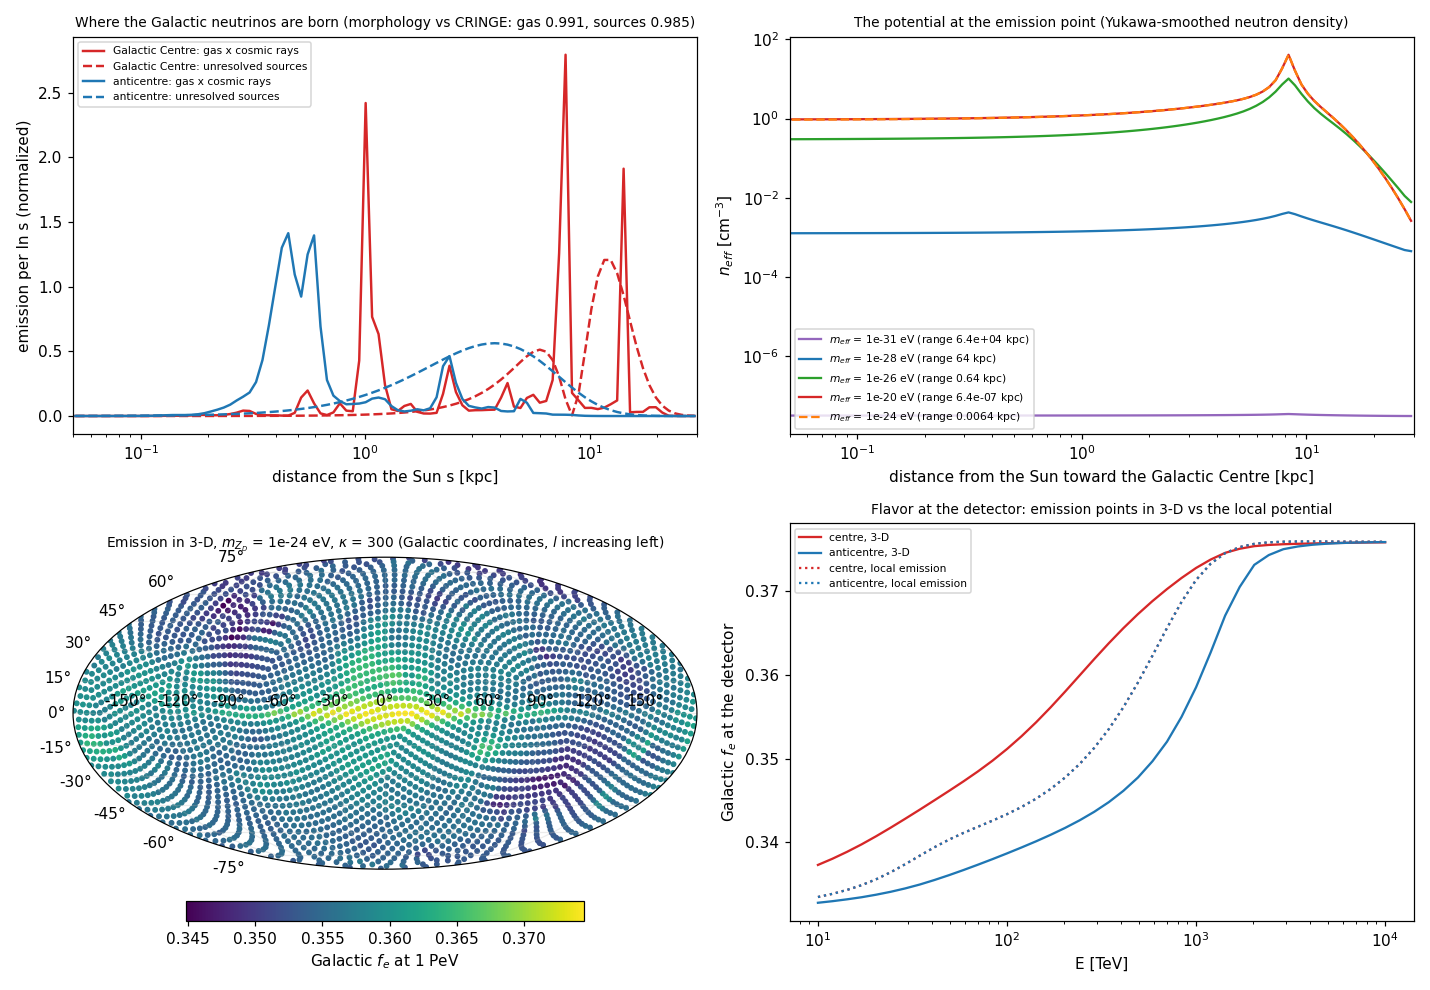
\includegraphics[width=\textwidth]{../output/figures/galactic_emission.png}
\caption{\textbf{Galactic emission points.} Top left: where along the lines of sight toward the Galactic
Centre and the anticentre the neutrinos are born, for the diffuse emission (gas times cosmic rays) and the
unresolved sources. Top right: the potential at the emission point along the Centre's line of sight for
several mediator ranges. Bottom: the Galactic $\nu_e$ fraction at the detector for emission points in 3-D at
$m_{Z_D} = 10^{-24}$~eV, per pixel at 1~PeV (left) and against energy for the Centre and the anticentre
(right; dotted: emission at the local potential).}
\label{fig:galactic_emission}
\end{figure}

\textit{The pieces together (plan step 7).}---To add the Galactic flux to the extragalactic one, the latter can
now be put in physical units (\texttt{sky.extragalactic\_norm}): its per-flavor intensity at 100~TeV without new
physics, from the closed form of the free-streaming flux, which the solver reproduces to its redshift grid's
first-order error ($4\times10^{-3}$ at 400 steps). With IceCube's HESE 7.5-year fit ($2.12\times10^{-18}$
GeV$^{-1}$~cm$^{-2}$~s$^{-1}$~sr$^{-1}$ per flavor at 100~TeV, $\gamma = 2.87$) the Galactic share of the flux
(CRINGE $\times$ 0.91) is 4\%, 6\% and 1\% of the sky-averaged flux at 10~TeV, 100~TeV and 1~PeV, and 22\%, 35\%
and 7\% in the inner Galaxy (Fig.~\ref{fig:sky_validation}). An independent check of the template's normalization:
at 20~TeV the sky-averaged CRINGE flux is 11\% of IceCube's 2026 astrophysical flux in that energy bin; the 2026
paper states ``about 10\%''. (HESE's soft fit lies a factor 4 above the 2026 flux at 10~TeV, the known tension
between it and fits with a spectral break, so the Galactic share depends on that choice.) At the dark-portal
point of Fig.~\ref{fig:galactic_emission} the anisotropy of $f_e$ at 100~TeV comes from the Galactic component
(a spread of 0.018 over the pixels; 0.014 in the total flux), against $10^{-6}$ from the Earth there and at most
$1.2\times10^{-3}$ from the Sun's yearly path (decision D4).

\begin{figure}[t]
\centering
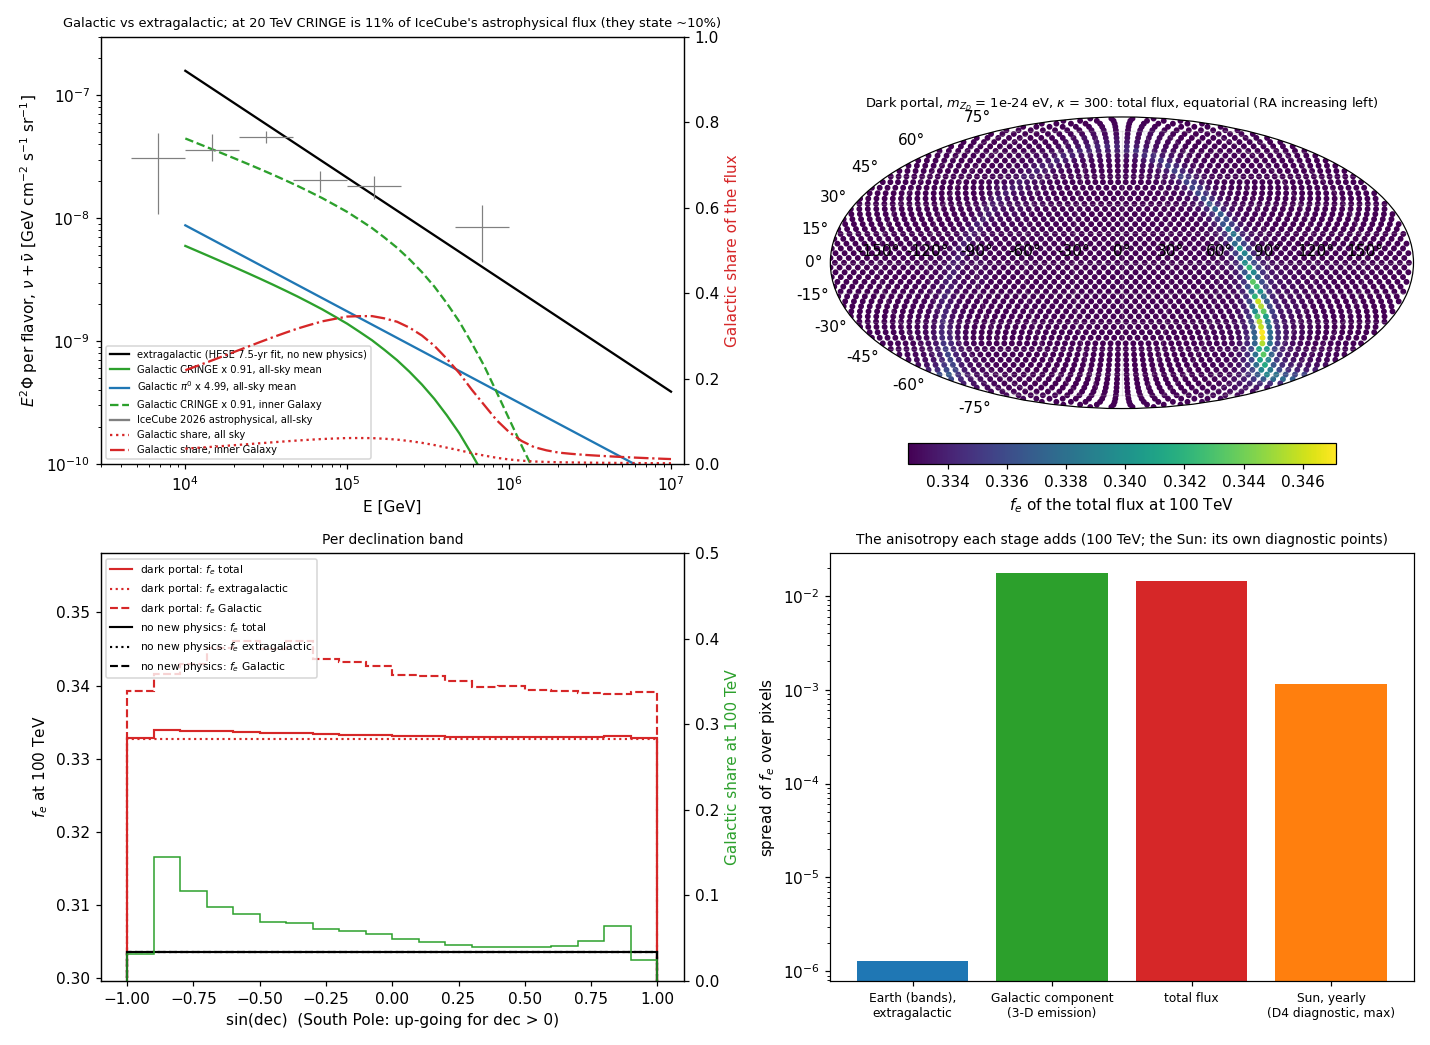
\includegraphics[width=\textwidth]{../output/figures/sky_validation.png}
\caption{\textbf{The sky with the Galactic component} (\file{tools/sky_validation.py}). Top left: sky-averaged
per-flavor spectra of the extragalactic flux (HESE 7.5-year fit), the Galactic templates and IceCube's 2026
astrophysical flux, with the Galactic share (right axis). Top right: $f_e$ of the total flux at 100~TeV for the
dark-portal point of Fig.~\ref{fig:galactic_emission}. Bottom left: per declination band, $f_e$ of the total,
extragalactic and Galactic fluxes with and without the dark portal, and the Galactic share. Bottom right: the
spread of $f_e$ over the pixels that each stage adds.}
\label{fig:sky_validation}
\end{figure}

\textit{A consumer: HESE (plan step 8).}---IceCube's HESE 7.5-year release gives each simulated event its weight
over flux and livetime, so its expected rate under a flux is the livetime times the sum over events of that
weight times the flux of the event's particle type at its true energy and direction (\file{tools/hese\_check.py};
the release on Tycho). With the release's best-fit flux (6.37 for the six species at 100~TeV, $\gamma = 2.87$)
our weighting and the release's own code (run in its own environment, with photospline for its detector
corrections) agree event by event to $2\times10^{-14}$: 50.16 astrophysical events above 60~TeV in 2635 days
(39.5 cascades, 8.4 tracks, 2.2 double cascades); the detector corrections at their nominal values are exactly 1.
The units test: \file{propagate\_sky} with sources $(1/3, 1/3, 1/3)$, which stay 1:1:1 at the Earth for any mixing,
and the extragalactic flux normalized to the same fit reproduces the release's flux for every one of the
736\,781 neutrino events to the same factor, 1.0036, the redshift grid's offset of the normalization: the
normalization, the neutrino--antineutrino split, the flavors, the declination
($\sin\delta = -\cos\theta_z$) and the energy interpolation are all consistent. Pion sources instead give the
flavors $(0.30, 0.36, 0.34)$ at the Earth: 3.7\% fewer cascades and 3.8\% more tracks. The Galactic component
(CRINGE $\times$ 0.91) adds 2.8 events (5.6\%), mostly cascades below 200~TeV (Fig.~\ref{fig:hese_check}).
Cascades resolve 10--20$^\circ$, so HESE can use maps of $N_{\rm side} = 8$ (Mauricio); the release's MC has no
azimuth, so the Galactic flux enters averaged over right ascension per declination band.

\begin{figure}[t]
\centering
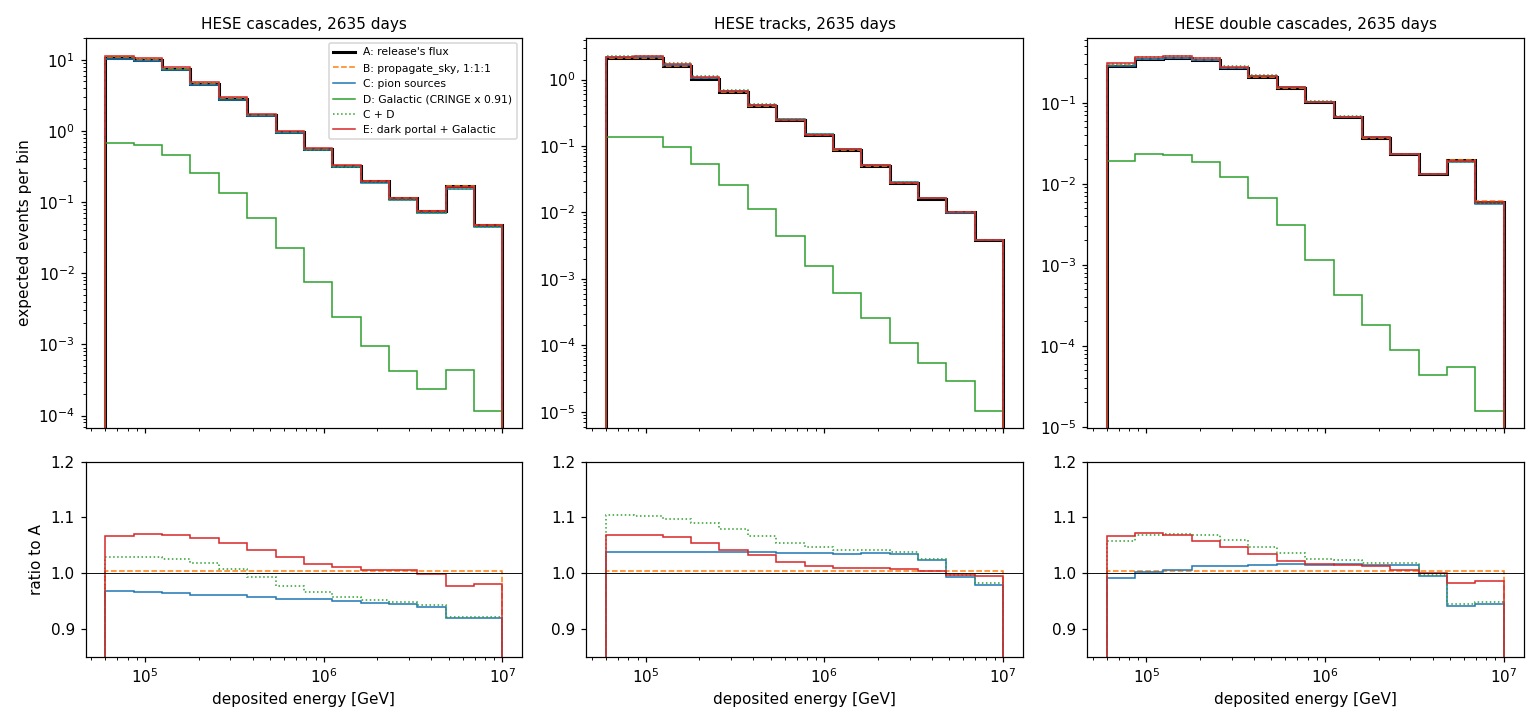
\includegraphics[width=\textwidth]{../output/figures/hese_check.png}
\caption{\textbf{Expected HESE events} (2635 days, deposited energy 60~TeV--10~PeV) per morphology, from the
release's MC: A, the release's best-fit flux; B, our per-direction output with sources 1:1:1 normalized to it
(the units test: 1.0036 for every event); C, pion sources; D, the Galactic component; E, a dark-portal point
with the Galactic component. Bottom: ratios to A.}
\label{fig:hese_check}
\end{figure}

\textit{The planes with the Galactic component (Mauricio's task 2; finished 2026-10-14).}---Every
secret-interaction plane and the pre-audit dark-portal planes were rerun with the Galactic component and
IceCube's 2026 spectrum as data (the extragalactic normalization and index floating; \file{tools/make_galactic_configs.py}),
with the sources' compositions at pion decay and, as a variant, fitted (Fig.~\ref{fig:galactic_comparison},
\file{tools/plot_galactic_comparison.py}). Read per mass as all planes are, the secret-interaction limits barely
move: the median ratio to the original limits is 1.02--1.23 per plane. Two findings. First, with the 2026
spectrum every secret-interaction plane prefers new physics somewhere: $\Delta\chi^2 = 3.6$--$10$ below the fit
without it, always for a resonance at 0.5--7.5~MeV (couplings $10^{-4}$--$10^{-1}$), the dip it carves fitting
the measured spectrum better than a power law ($\sim$2$\sigma$ for the two parameters); the same will show in the
MeV planes of the campaign. (The comparison tool had first dropped every mass column whose minimum lies above
the plane's, which this preference makes all of them; fixed.) Second, fitting the sources' compositions instead
of fixing them at pion decay weakens the limits below $\sim$1~MeV by 1.5--10 times. The dark portal's planes of
this task predate the physics audit (Sec.~\ref{sec:audit}) and are superseded by the campaign; its last four
dark-portal analyses (the FrequentistAnalysis ports, with the mixing free) were stopped, with Mauricio's agreement.

\begin{figure}[t]
\centering
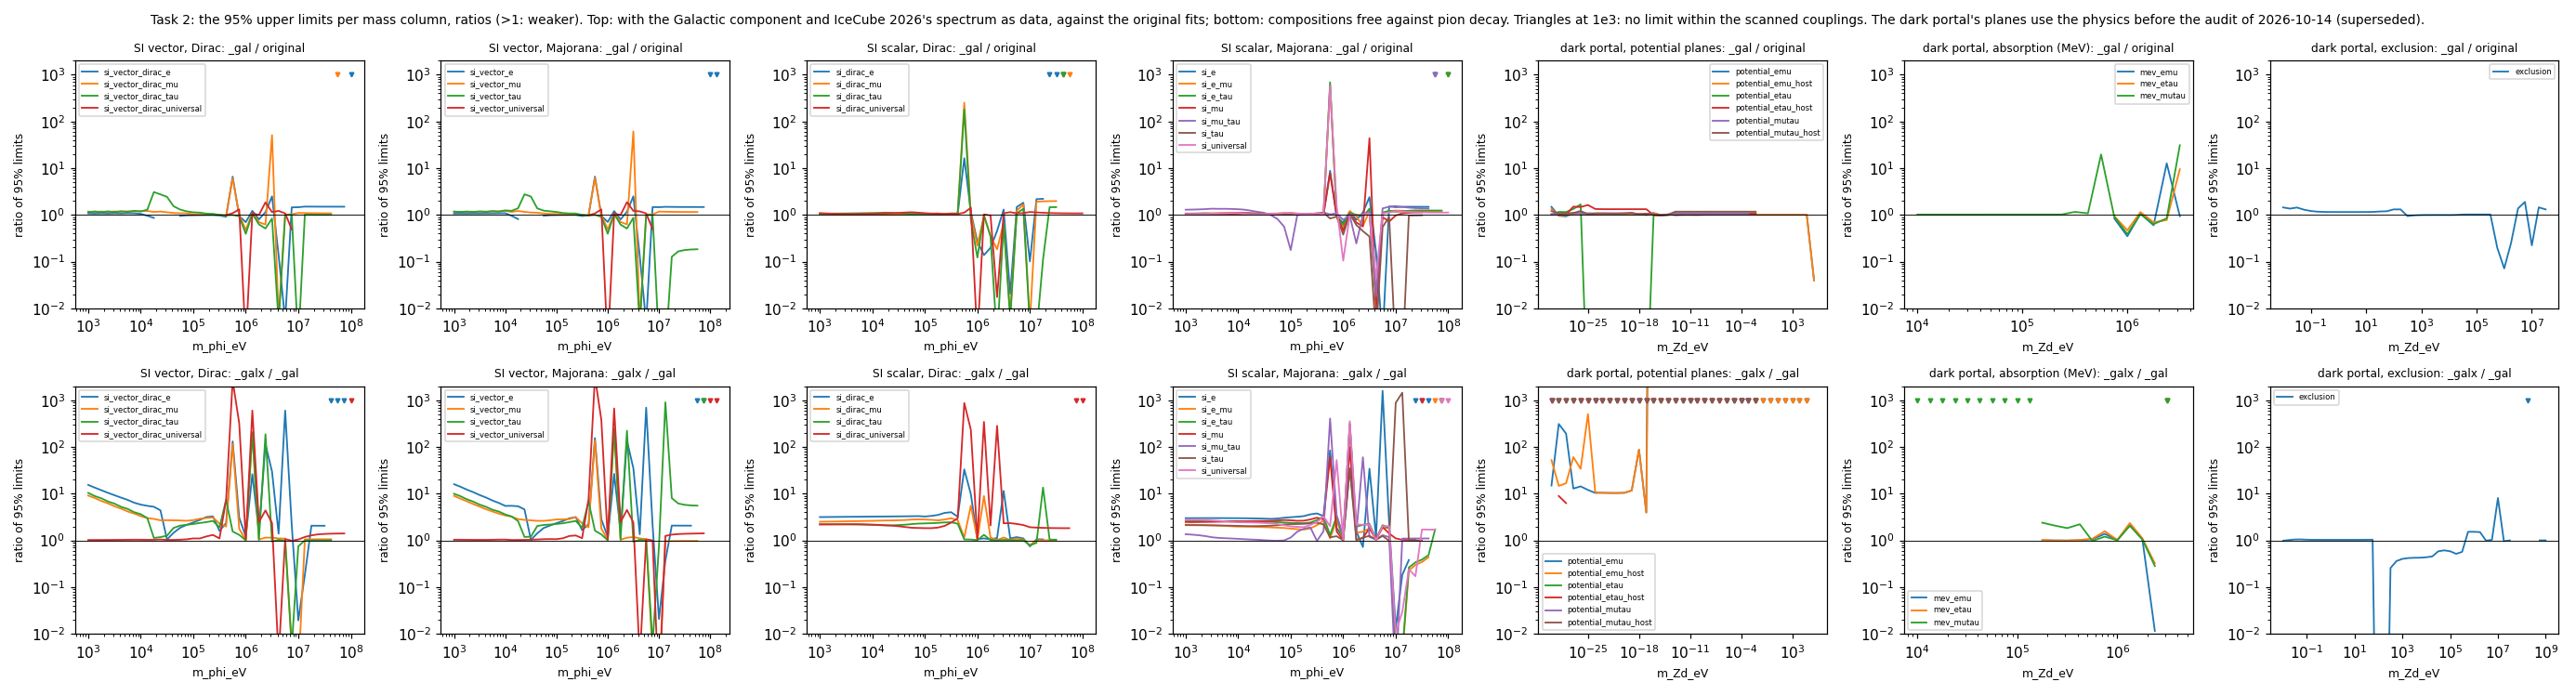
\includegraphics[width=\textwidth]{../output/figures/galactic_comparison.png}
\caption{\textbf{Task 2: the Galactic component and IceCube's 2026 spectrum.} The 95\% upper limits per mass,
as ratios (above 1: weaker). Top: with the Galactic component and the 2026 spectrum as data, against the
original flavor-only fits. Bottom: the sources' compositions fitted, against pion decay. The dark portal's
panels use the physics before the audit (superseded).}
\label{fig:galactic_comparison}
\end{figure}

\section{Track rates with IceTracks-DR2}
\label{sec:dr2}

Expected through-going muon tracks for any flux the solver computes (\file{IceCubeRates/}; plan in
\file{docs/dev/DR2\_TRACKS\_PLAN.md}). The response is IceCube's IceTracks-DR2 release (v3.1, 2008--2022,
doi:10.7910/DVN/MMIIZA), in four detector configurations: IC40, IC59, IC79 and IC86 (eleven seasons), 4963 days
of good runs in all. For each it gives the muon-neutrino effective area $A(E_\nu, \delta)$, in 0.2-dex bins of
true energy and 50 bins of true declination (uniform in $\sin\delta$), with absorption in the Earth included,
and a five-dimensional smearing table: for each bin of true energy (0.5 dex) and declination (30--52 bins), the
fraction of simulated events in each cell of reconstructed muon energy, point-spread angle $\psi$ (between the
true neutrino direction and the reconstructed muon direction) and estimated angular error. We sum over the
angular error and move the cells, which the release chooses per bin, onto common grids: 0.1~dex in reconstructed
energy and 0.25~dex in $\psi$ up to $180^\circ$, in proportion to their overlaps (\file{tools/dr2\_reduce.py}).
Every filled slice still sums to 1, to $4\times10^{-13}$.

\textit{The fold.}---For configuration $c$, with livetime $T_c$, the expected number of tracks in a bin of
reconstructed energy $E_r$ and reconstructed declination $m$ is
\begin{equation}
N_c(E_r, m) = T_c \sum_{i,k} A_c(i,k) \int_{E_i}\!dE \int_{\delta_k}\!d\Omega\; \Phi_{\nu_\mu+\bar\nu_\mu}(E,\delta)
\sum_q P_c(E_r, \psi_q \,|\, i, k)\, G(k, q, m) \;,
\end{equation}
with $i, k$ the effective area's bins (the smearing's bins hold their centres) and $G$ the geometry: the
probability that a track from true bin $k$, deflected by $\psi$ in bin $q$ at an azimuth uniform around the true
direction, is reconstructed in bin $m$. On the sphere, $\sin\delta_r = \sin\delta\cos\psi + \cos\delta\sin\psi\cos\phi$;
for an edge $\delta_e$ the probability $F = P(\delta_r < \delta_e) = 1 - \arccos(c)/\pi$, with
$c = (\sin\delta_e - \sin\delta\cos\psi)/(\cos\delta\sin\psi)$ clipped to $[-1, 1]$, is exact in the azimuth. As a
function of the true declination, $F$ is flat (0 or 1) or smooth between four breakpoints, $\delta_e \mp \psi$ and
$\pm(180^\circ - \psi) - \delta_e$, where the circle of radius $\psi$ reaches the edge directly or over a pole, with
square-root ends there; we split each true bin at them and integrate each piece by Gauss--Legendre with nodes
clustered at its ends, and integrate $\log\psi$ within each bin with nodes at most $0.5^\circ$ apart. Against Monte
Carlo (tracks uniform in $\sin\delta$ within a bin, $\psi$ log-uniform, azimuth uniform) the kernel agrees within
the statistics everywhere: the worst of 1584 comparisons is $2.8\sigma$. A first version, plain Gauss--Legendre in
$\sin\delta$, was wrong by 6--9\% wherever an edge cut a true bin, and then by 1.5\% for $\psi$ near $180^\circ$ at
the poles; the Monte Carlo test caught both. The point-spread angle moves 0.1--0.3\% of an isotropic flux's tracks
across $\delta = -5^\circ$, and conserves the total.

\textit{The atmospheric background.}---As in NuFlavorSingleSource (Mauricio, 2026-10-14): MCEq with SIBYLL-2.3d and
the H3a cosmic rays gives the nominal flux, conventional plus prompt, and its derivatives with respect to the
twelve hadron-production parameters of Barr et al.\ that matter above 30~GeV (pions in regions G, H, I and kaons
in W, Y, Z, each charge separately; priors 0.30, 0.15, 0.122 and 0.40, 0.30, 0.122) and to a tilt of the cosmic-ray
spectral index (prior 0.05); the prompt normalization varies with prior 0.5. The flux is linear in all of them,
$\Phi = \Phi_0\,(1 + \sum_p \theta_p\, \partial_p \ln\Phi) + \theta_{\rm pr}\Phi_{\rm pr}$, so each enters a fit as one
folded template. The regions, priors, yield modification and cosmic-ray tilt are NuFlavorSingleSource's code,
copied unchanged (\file{tools/atmospheric\_background.py}); for IceCube we use the South Pole's atmosphere
(NRLMSISE-00, January and July averaged) instead of the US standard one, and 20 production zenith angles dense near
the horizon instead of 8. A two-angle test reproduces NuFlavorSingleSource's relative derivatives to $10^{-3}$;
only the prompt fraction differs (0.185 against 0.197 at 100~TeV, vertical), from the atmosphere. Up-going
directions take the flux produced at the mirror zenith on the far side. daemonflux (MCEq calibrated to muon data)
is kept as a cross-check of the conventional flux.

\textit{Against the data.}---With the nominal atmospheric flux and IceCube's 9.5-year fit of the astrophysical
flux ($\nu_\mu+\bar\nu_\mu$: $1.44\times10^{-18}$ GeV$^{-1}$~cm$^{-2}$~s$^{-1}$~sr$^{-1}$ at 100~TeV, $\gamma = 2.37$),
the tracks reconstructed above $\delta = -5^\circ$ number 1.057, 1.155, 1.067 and 1.123 times our expectation in IC40,
IC59, IC79 and IC86 (Fig.~\ref{fig:dr2_validation}): the units are right, and the declination distribution is flat
in the ratio. Split by declination and energy, IC79 and IC86 agree above 3~TeV (IC86 is 15\% high below, the
overall normalization). The early configurations do not: IC40 has twice the expected events above 3~TeV, but only
within $10^\circ$ of the horizon (atmospheric muons reconstructed as up-going, absent from our model), and IC59 has
1.2--1.8 times the expected events above 3~TeV at every declination, even above $+40^\circ$, where muons cannot
reach: its published responses and its events disagree at high energy. A fit of the atmospheric nuisances (and of a
normalization per configuration and the astrophysical flux) to IC79 and IC86 cannot absorb the rest: with $10^6$
events every bin is measured to better than 1\%, and the fit pulls Barr parameters by up to $13\sigma$ to mimic what
are detector effects, for which DR2 publishes no systematics. A track likelihood will therefore need detector
nuisances (a normalization and an energy scale per configuration) or an energy threshold above which the
astrophysical flux matters and the data and our expectation agree; IC40 and IC59 are left out until then.

\begin{figure}[t]
\centering
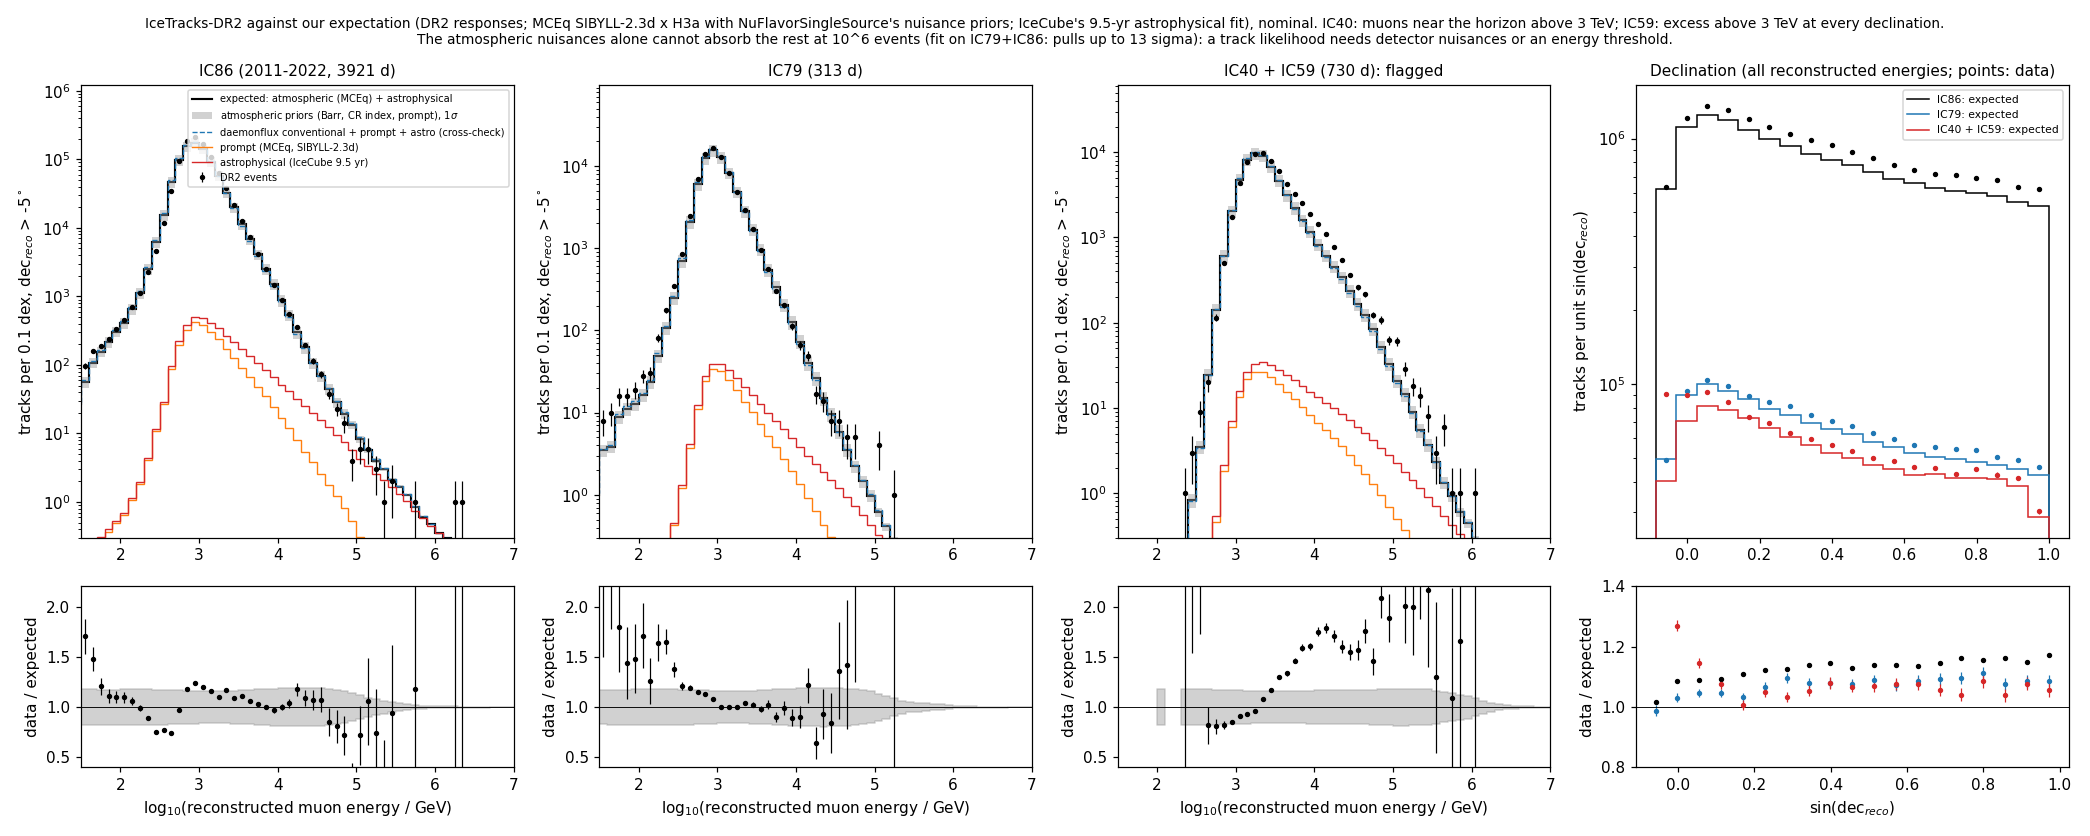
\includegraphics[width=\textwidth]{../output/figures/dr2_validation.png}
\caption{\textbf{IceTracks-DR2 against our expectation} (\file{tools/dr2\_validation.py}): tracks reconstructed above
$\delta = -5^\circ$ in reconstructed muon energy for IC86, IC79 and IC40 + IC59, and in declination; the expectation
is the DR2 responses folded with our atmospheric flux (MCEq SIBYLL-2.3d $\times$ H3a at the South Pole; band: the
Barr, cosmic-ray and prompt priors) and IceCube's 9.5-year astrophysical fit, at nominal values; dashed:
daemonflux's conventional flux instead.}
\label{fig:dr2_validation}
\end{figure}

\textit{New physics in the tracks.}---The solver's flux per declination band (the effective area's 50 bands, the
Galactic component from $N_{\rm side} = 64$ data), with the extragalactic $\nu_\mu+\bar\nu_\mu$ normalized to the
9.5-year fit without new physics (pion sources put 35.5\% of the flux in $\nu_\mu$ at the Earth: the flavor-averaged
normalization times 0.938; the solver's standard tracks then equal the fit's power law in every bin, to $5\times10^{-15}$),
gives 3835 extragalactic and 527 Galactic tracks above $\delta = -5^\circ$ in 2008--2022, 340 and 23 of them above
10~TeV reconstructed (Fig.~\ref{fig:dr2_tracks}). The dark-portal point of Fig.~\ref{fig:galactic_emission} removes
6\% of the extragalactic tracks at every energy (its flavor composition), the secret-interaction point ($\nu_\tau$,
5~MeV, $g = 0.05$) 43\% at 200~TeV reconstructed (absorption near the resonance) while adding 5--10\% below 10~TeV
(the regenerated neutrinos). The Galactic share of the tracks is 12\% in all, 6\% above 10~TeV.

\begin{figure}[t]
\centering
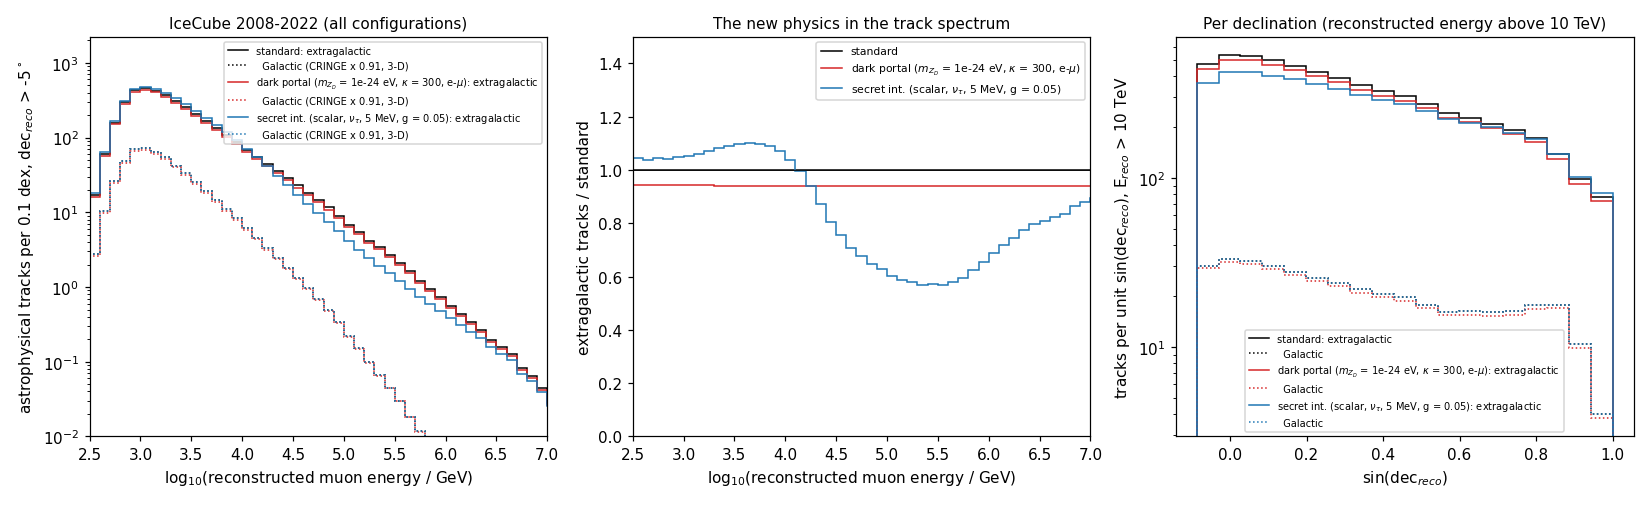
\includegraphics[width=\textwidth]{../output/figures/dr2_tracks.png}
\caption{\textbf{Astrophysical tracks with new physics} (IceCube 2008--2022, all configurations, reconstructed
$\delta > -5^\circ$): extragalactic (solid) and Galactic (dotted) for standard physics, a dark-portal point and a
secret-interaction point; their ratio to standard; per declination above 10~TeV.}
\label{fig:dr2_tracks}
\end{figure}

\section{Starting events with HESE}
\label{sec:hese}

Expected HESE events (Mauricio's task 1; plan in \file{docs/dev/HESE\_RATES\_PLAN.md}) from IceCube's 7.5-year release:
its simulated events weighted per event by any flux, exactly (Section~\ref{sec:directions}'s consumer check), in the
release's binning (cascades and tracks in deposited energy and zenith, double cascades in deposited energy and
length), with the release's cuts (\file{tools/hese\_reduce.py}: 736\,814 simulated events; the 60 events above
60~TeV: 41 cascades, 17 tracks, 2 double cascades). The release's best-fit astrophysical flux gives 50.16 events
(39.51, 8.43, 2.21), as before.

\textit{Backgrounds.}---The atmospheric neutrinos are our MCEq flux (Section~\ref{sec:dr2}) per event, the
conventional part times the release's conventional self-veto correction and the prompt part times its prompt one
(Mauricio, 2026-10-14). The conventional part agrees with the release's own model (Honda-based, its veto) to 5\% in
every morphology: 7.91 events against 8.01. The prompt part, from SIBYLL-2.3d, is 3.04 events against the
release's 1.63 (BERSS): the known difference of the two charm models, within its 50\% prior. The atmospheric muons
are the release's own simulation, 0.79 events (tracks).

\textit{Detector systematics.}---The release corrects each event's weight for the DOM efficiency (prior
$0.99\pm0.1$), the head-on efficiency ($0\pm0.5$) and the ice anisotropy ($1\pm0.2$), with splines per flux
component. We export the exact weights from the release's own code, run in its own environment, on a grid of each
systematic's values per event (\file{tools/hese\_detector\_systematics.py}) and interpolate between them. At
$+1\sigma$ the DOM efficiency moves the expectation by 7.3 cascades, 1.6 tracks and 0.4 double cascades; the other
two by 0.1 events or less.

\textit{Expectation against the data.}---With the release's astrophysical fit and our backgrounds, we expect
$45.8\pm7.6$ cascades, $13.7\pm2.1$ tracks and $2.4\pm0.4$ double cascades (detector and atmospheric $1\sigma$,
correlated across bins; Fig.~\ref{fig:hese_rates}), against 41, 17 and 2.

\begin{figure}[t]
\centering
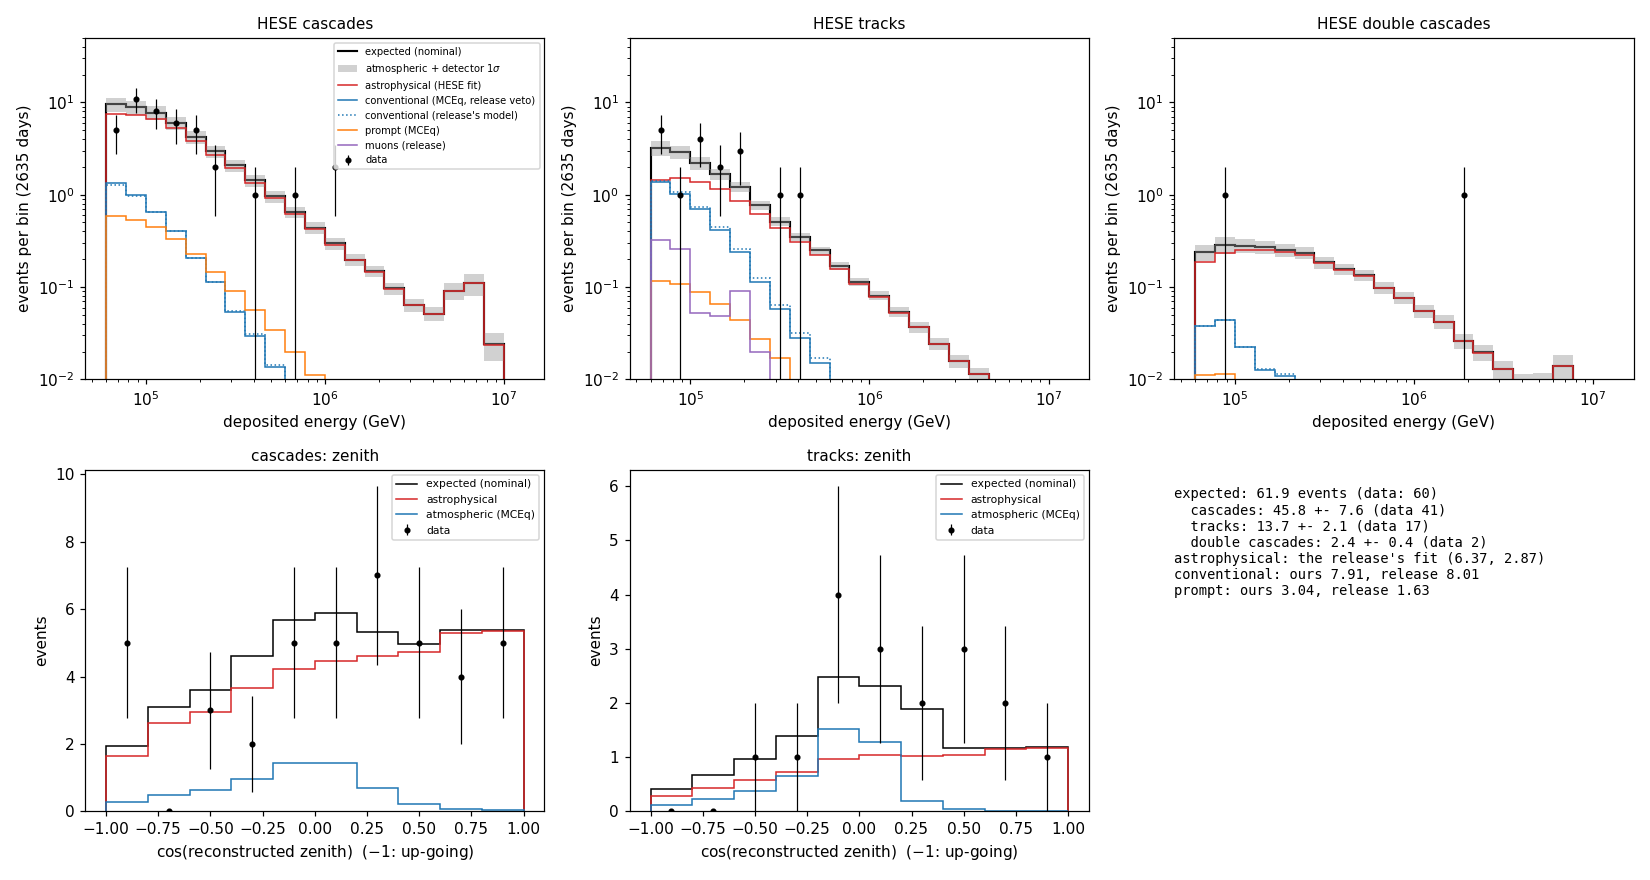
\includegraphics[width=\textwidth]{../output/figures/hese_rates.png}
\caption{\textbf{HESE events against our expectation} (\file{tools/hese\_rates.py}): per morphology in deposited
energy, and in zenith for cascades and tracks; the astrophysical flux is the release's fit, the atmospheric
neutrinos our MCEq flux with the release's self-veto (dotted: the release's own conventional model), the muons the
release's; band: the atmospheric and detector $1\sigma$.}
\label{fig:hese_rates}
\end{figure}

\textit{New physics in HESE.}---With the extragalactic flux normalized to the release's fit and pion sources, standard
physics gives 38.1 cascades, 8.75 tracks and 2.23 double cascades, and the Galactic component 2.25, 0.46 and 0.11
(Fig.~\ref{fig:hese_cases}). The dark-portal point moves 4\% of the events from tracks to cascades. The
secret-interaction point removes 35\% of the cascades and half of the tracks and double cascades: HESE's energies,
60~TeV--10~PeV deposited, sit at the resonance, where the northern tracks (mostly below 100~TeV) lose 14\% above
10~TeV.

\begin{figure}[t]
\centering
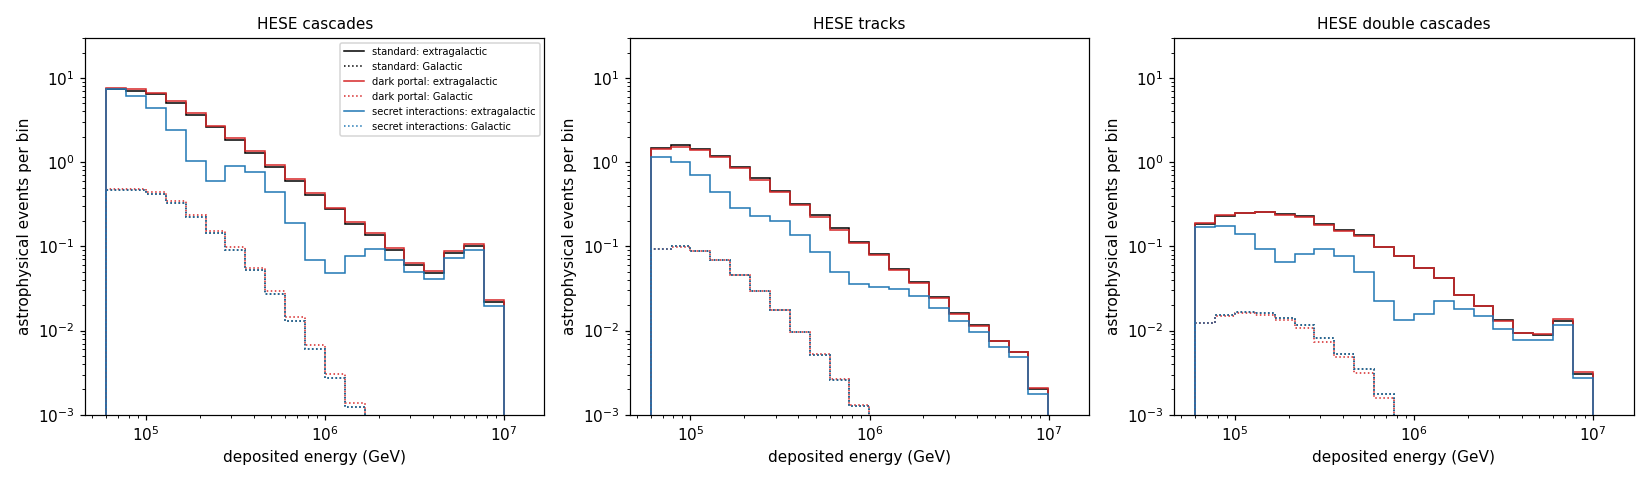
\includegraphics[width=\textwidth]{../output/figures/hese_cases.png}
\caption{\textbf{HESE events with new physics}: extragalactic (solid) and Galactic (dotted) per morphology for
standard physics, a dark-portal point and a secret-interaction point.}
\label{fig:hese_cases}
\end{figure}

\section{Matter charges and textures: the scope of the dark-portal paper}
\label{sec:scope}

\textit{Decisions (Mauricio, 2026-10-14).}---The dark-portal paper widens the model in two ways and
claims, in its abstract, the most comprehensive calculation of these effects in high-energy
astrophysical neutrinos, with several kinds of current data. Working title: ``New forces on
high-energy cosmic neutrinos, from the Hubble scale to the Earth''. First, a general matter charge:
the potential is sourced by $q_n n_n + q_p n_p + q_e n_e$, not by neutrons alone. Second, a family of
neutrino textures. Eight benchmark models, each with the matter charge and the texture its gauge
structure fixes (Table~\ref{tab:benchmarks}). The dark portal's mixing ratios are free, with full planes
for named textures (pure $e$, $\mu$, $\tau$; $e\mu$, $e\tau$, $\mu\tau$; democratic) and maps of the
bound over the ratio triangle at a few masses. The plan is \file{docs/dev/SCOPE_WIDENING_PLAN.md}.

\begin{table}[h]
\centering
\caption{\textbf{The eight benchmark models.} Matter charges in neutral matter ($n_p = n_e$);
neutrino charges $(e,\mu,\tau)$. The first three gauge models are those of
Agarwalla, Bustamante, Das \& Narang (JHEP 08 (2023) 113).}
\label{tab:benchmarks}
\footnotesize
\begin{tabular}{lll}
\toprule
Model & Matter charge & Neutrino texture \\
\midrule
Dark portal & neutrons ($Z$--$Z_D$ mixing) & $uu^\dagger$, ratios free \\
$L_e-L_\mu$, $L_e-L_\tau$ & electrons & $(1,-1,0)$, $(1,0,-1)$ \\
$L_\mu-L_\tau$ & neutrons ($Z$--$Z'$ mixing) & $(0,1,-1)$ \\
$B-3L_e$ & $n - 2e$ & $(-3,0,0)$ \\
$B-3L_\mu$, $B-3L_\tau$ & nucleons & $(0,-3,0)$, $(0,0,-3)$ \\
$B-\frac{3}{2}(L_\mu+L_\tau)$ & nucleons & $(0,-\frac{3}{2},-\frac{3}{2})$ \\
\bottomrule
\end{tabular}
\end{table}

\textit{Conventions.}---The theory notes' $\epsp$ (T9, T12) is half the dark-$Z$ mixing $\epsilon_Z$ of
Davoudiasl, Lee \& Marciano, whose neutron coupling is $\epsilon_Z g/(4c_W)$; the notes' neutron coupling
$\epsp g/(2c_W)$ and neutrino coupling $\epsp g/c_W$ (T12) follow one normalization, so the model is
self-consistent. For $L_\mu-L_\tau$, whose $Z'$ reaches the neutrons by the same mixing, the 2023 paper's
$\xi$ is $2\epsp$.

\textit{The matter charge (step 1, done).}---In neutral matter $n_p = n_e$, so only $q_n$ and
$q_p + q_e$ enter. Every density the solver uses is linear in its source, so each is computed for
neutrons and for electrons and combined (\file{src/dp_matter.py}): the cosmic mean
($n_{e,0} = n_b(1 - Y_p/2) = 2.2059\times10^{-7}$~cm$^{-3}$), the Galaxy at the Sun and at its emission
points (electrons per nucleon $0.80$ in stars, $0.858$ in cold gas; the hot halo's profile is already
the electron density), the Sun, the Moon and the Earth's Yukawa profile ($Y_e$ by layer, water on top).
The electrons per body are $1.0046\times10^{57}$ (Sun), $1.7480\times10^{51}$ (Earth, PREM integrated)
and $2.1895\times10^{49}$ (Moon). The solver carries the potential's sign in its coefficient, so a
charge negative in every body ($B-3L_e$) has its sign moved there, and one that changes sign between
bodies is refused. Fig.~\ref{fig:matter_sources} shows what changes: the distant sources are rich in
hydrogen, with four to seven electrons per neutron, while the Earth and the Moon have about one. An
electron-sourced force therefore weighs the potential at IceCube $7.1$ times the neutrons' at cosmic
ranges, $4.2$ at Galactic ones and $4.4$ where the Sun dominates (from an AU to a kiloparsec), but $0.95$ at
the Earth's. Checks (\file{tests/test_matter_charge.py}, 16 tests): linearity of every density to
$10^{-12}$; the electron counts against the bodies' masses; the general path with the neutron charge
equal to the historical one to $10^{-12}$; a negative charge equal to a flipped texture. The four
validation points are bit for bit those of the previous code, compiled fresh on both sides (a cached
and a fresh build of the same code already differ by $7\times10^{-15}$).

\begin{figure}[t]
\centering
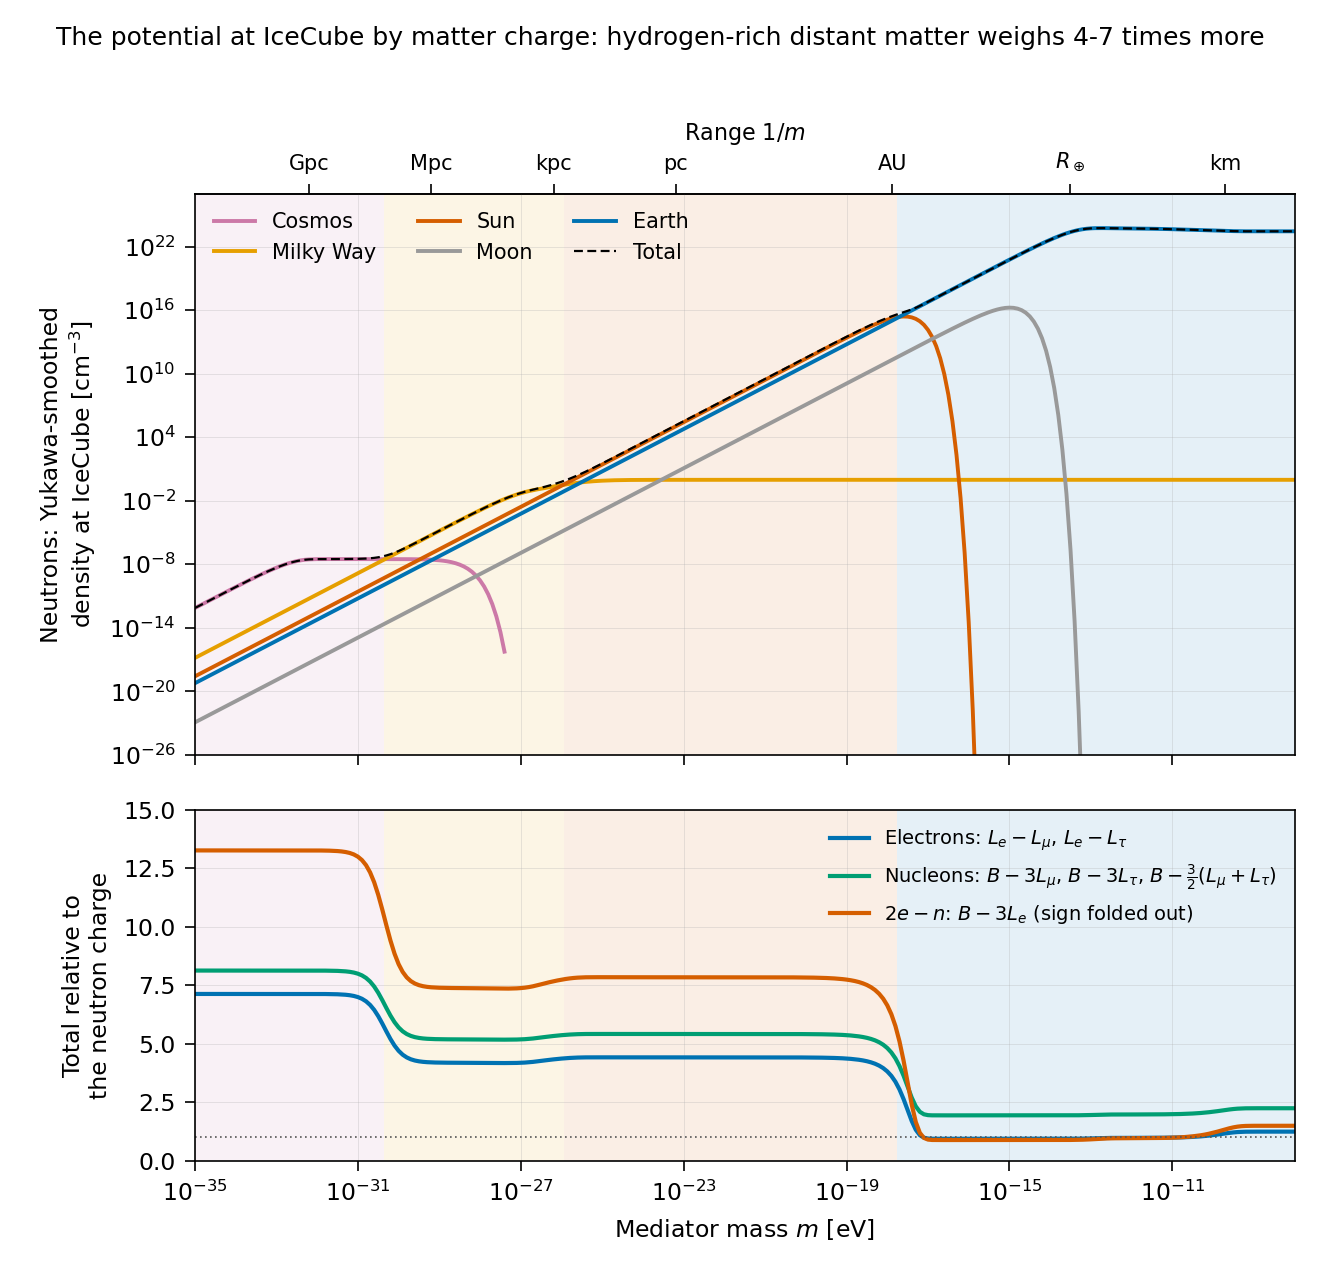
\includegraphics[width=0.85\textwidth]{../output/figures/matter_charge_sources.png}
\caption{\textbf{Where the potential at IceCube comes from.} Top: the Yukawa-smoothed neutron density
at the detector per body versus the mediator mass (shading: the dominant body). Bottom: each benchmark
charge's total relative to the neutrons'. \file{tools/plot_matter_sources.py}.}
\label{fig:matter_sources}
\end{figure}

\textit{The absorption counted every relic state in full (found 2026-10-14).}---The resonant absorption
(T7, T11, T12; \file{src/dp_thermal.py}) gives an incident $\nu_\alpha$ the same coupling
$(\Sigma G)_\alpha$ with each of the three relic mass states. A relic state offers only its own flavor
components: the $s$-channel amplitude of $\nu_\alpha + \bar\nu_i$ is $(CU^*)_{\alpha i}$, with $C$ the
coupling matrix in the flavor basis, and summed over the three states this gives $(CC^\dagger)_{\alpha\alpha}
= (\Sigma G)_\alpha$, one species' worth of targets where the kernel counts three. The width is the same in both. With
the kernel itself, a flavor-diagonal coupling absorbs $\nu_e$ as strongly on the heaviest state as on
the lightest, although $|U_{e3}|^2 = 0.02$; integrated over energy, the absorption is $2.9$ times too
strong for the dark portal's $e\mu$ texture and $2.2$ ($\nu_e$) and $4.2$ ($\nu_\mu$) for $L_e - L_\mu$
(Fig.~\ref{fig:relic_weights}). Mauricio decided (2026-10-14) to weigh each state by its own flavor
content, $|(CU^*)_{\alpha i}|^2$, for all eight models, and the Debye mass likewise; the dark portal's
MeV planes will change, by up to $\sqrt3$ in $g_D|U|^2$. This departs from the theory notes.

\begin{figure}[t]
\centering
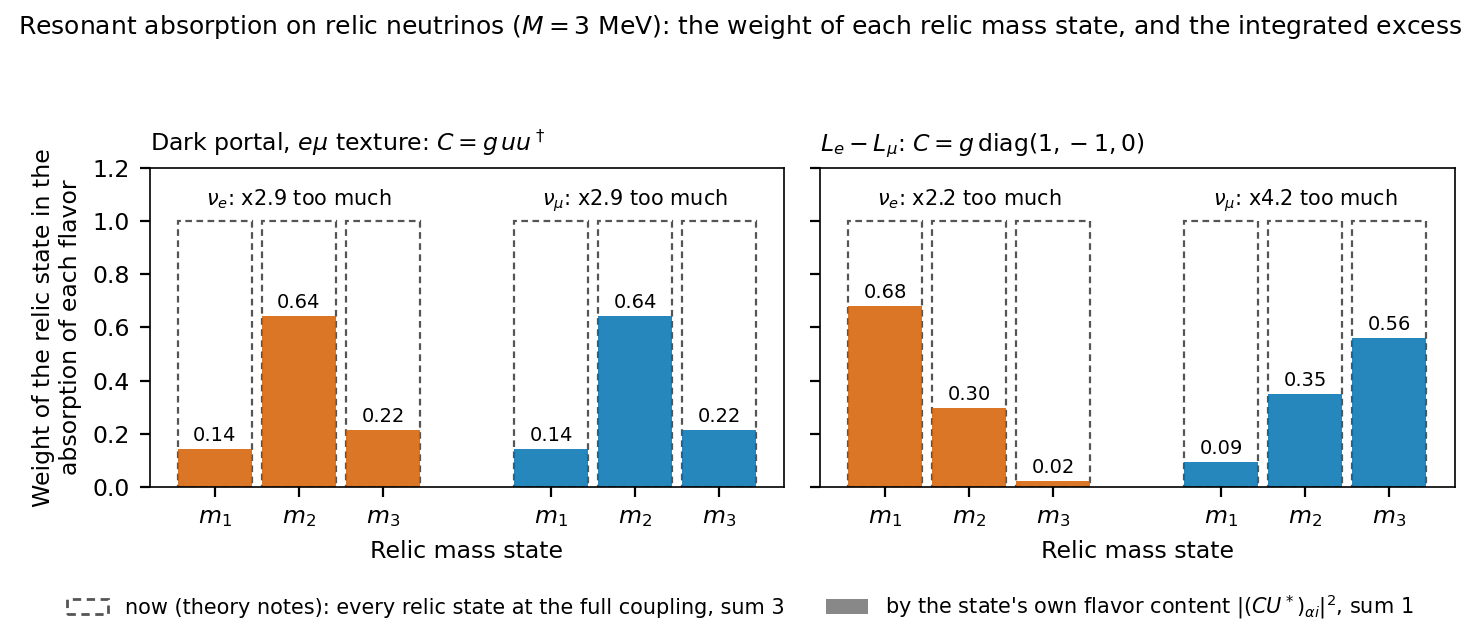
\includegraphics[width=0.85\textwidth]{../output/figures/absorption_relic_weights.png}
\caption{\textbf{How the absorption weighs the relic mass states} at $M = 3$~MeV: as computed until
2026-10-14 (dashed, every state at the full coupling) and by each state's flavor content (bars).
\file{tools/absorption_relic_weights.py}.}
\label{fig:relic_weights}
\end{figure}

\section{The physics audit of 2026-10-14}
\label{sec:audit}

Mauricio asked, before any further runs, for every part of the physics code to be checked
(\file{docs/dev/PHYSICS_AUDIT.md} lists each item with its derivation or check). The propagation chain
holds: the cosmological evolution and injection, the adiabatic Galaxy, the coherent Sun, the Earth's Yukawa
profile and chords, the matter models, the flux assembly and the event folds. A new absolute check: with a
potential far above the vacuum term everywhere and no absorption, the composition at the Earth is
$\sum_a|W_{\alpha a}|^2\sum_f|W_{fa}|^2 f_f$ with $W$ the texture's eigenvectors (its null space split by
the projected vacuum term), and the solver reproduces it to $10^{-11}$ for three textures, neutrinos and
antineutrinos. The errors were all in the resonant absorption on the relic neutrinos, which followed the
theory notes' Eqs.~(T7), (T11), (T12).

\textit{The absorption, from the Lagrangian.}---With the mediator coupled to the neutrinos as
$V_\mu\sum G_{\alpha\beta}\bar\nu_\alpha\gamma^\mu P_L\nu_\beta$ ($G = g_D uu^\dagger$ for the dark portal, in
the coupling of Eq.~(T9)), an incident eigenstate $a$ (flavor amplitudes $W_{fa}$) meets the relic mass
state $r$ with amplitude $(U^\dagger GW)_{ra}$, and the Breit--Wigner of a vector formed by
$\nu_L+\bar\nu_R$ integrates to $2\pi|(U^\dagger GW)_{ra}|^2$ per target, the normalization of the
$Z$-burst. The code gave every relic state the full flavor coupling (three times the targets), counted each
neutrino pair with the width of a Dirac pair with vector couplings, $M/12\pi$, instead of the left-handed
one, $M/24\pi$ (twice the rate per target), and projected eigenstates and secondaries on flavor without
interference. A flavor-universal coupling, diagonal in the mass basis, must absorb mass state $j$ only on
relic state $j$; the old form spread it over all three. Mauricio decided (2026-10-14) on the Lagrangian form
throughout: each relic state by its own flavor content, coherently per eigenstate, the left-handed width,
the decays' neutrinos in the eigenstates by $(W^\dagger GG^\dagger W)_{aa}$
(\file{src/dp_absorption.py}). At $3$~MeV and $g_D|U|^2 = 2.5\times10^{-4}$ the deepest dip goes from
$0.003$ to $0.021$ of the flux, and much of the old flavor shift disappears. I wrote the 2026-10-12
normalization from Eq.~(T11) as it stands; its $Z$-burst check held only with the $Z$'s coupling divided by
$\sqrt2$.

\textit{The $Z$ mixing in the absorption.}---Eq.~(T12)'s term $c\,\epsp g/c_W$ is the cross term of
$|c+\kappa|^2$ with $\kappa = \epsp g/c_W$, the coupling the $Z$--$Z_D$ mixing gives every neutrino, but it
drops $\kappa^2$ and puts the cross term on every flavor pair. Mauricio decided to keep all three pieces:
$G = g_Duu^\dagger + \kappa I$, with the $e^+e^-$ and $\mu^+\mu^-$ decays of the mixing in the width. Then
$\epsp = 0.1$ alone absorbs every flavor near MeV masses, and the potential planes no longer depend on
$P = \gd\epsp|U|^2$ alone: they will profile $\epsp$ (decided).

\textit{Relics in motion.}---The kernel used the massless relic's flux factor $1-\cos\theta$; the Moller
factor of a relic at speed $v$ is $1-v\cos\theta$, which changes the integrated absorption by $+1.7\%$,
$+1.3\%$ and $+0.3\%$ for the three states at $m_{\rm lightest} = 0.01$~eV and $+9\%$ for a $10^{-3}$-eV
lightest state.

\textit{Screening (a departure from Eq.~T9).}---The relics' Debye mass, Eq.~(T23), is the relativistic one,
$m_D^2 = \sum_r|G'_{rr}|^2T^2/6$ ($G' = U^\dagger GU$). Today's relics are slow, and the mediator couples to the
left-handed current, so a relic's charge depends on its speed $v$. The vector current of a Majorana field
vanishes, and its left-handed current is $-\tfrac12\bar\nu\gamma^\mu\gamma_5\nu$, whose charge on a state of
helicity $h$ is $-G'_{rr}hv$: a slow Majorana neutrino carries almost no charge. The static polarization
$\sum\int d^3p/(2\pi)^3\,q^2(-\partial f/\partial E)$ then gives $9\zeta(3)|G'_{rr}|^2T^3/(2\pi^2m_r)$ per
state, smaller than Eq.~(T23) by $3.3\,T/m_r$ (a Dirac relic's charge is $(1+v)/2$, giving
$|G'_{rr}|^2m_rT\ln2/(4\pi^2)$). The code takes Majorana relics, as for the absorption's targets; the $Z$
mixing's piece is $m_D\approx2\times10^{-5}$~eV$\times\kappa$ today. Screening needs the relics to move:
around the Earth, the Moon, the Sun and the Galaxy they drift in the potential's gradient (they cross the
Galaxy in $\sim10^7$~yr), but the uniform cosmological potential pushes on none of them and could only be
screened if the relic background acquired net dark charge everywhere at once, which charge conservation
forbids (the uniform background of the ``jellium'' model is not screened either). We therefore screen the
localized bodies only, and the cosmological potential keeps the bare mediator mass; Eq.~(T9) screens it too.
At $\epsp = 0.1$ the screening mass is $\sim2\times10^{-6}$~eV (a range of $\sim12$~cm) and cuts off every
ultralight local potential; at $\mzd = 10^{-20}$~eV, $\epsp$ and $\gd|U|^2$ must both stay below
$\sim5\times10^{-16}$ for those potentials to act. Since the potential fixes only $P = \gd\epsp|U|^2$, a split
with a large $\gd|U|^2$ and a tiny $\epsp$ switches off the Earth, the Sun and the Galaxy (today, for a mediator
lighter than the inverse distance: $\gd|U|^2 > 2\times10^{-9}$, $7\times10^{-14}$, $4\times10^{-23}$), and no
published limit forbids it: MICROSCOPE bounds $\epsp < 3\times10^{-25}$ from above, and cosmology bounds a
neutrino-only coupling only at $\sim10^{-7}$. Mauricio decided that each potential plane shows two curves: the bound
on $P$ where screening is negligible, which does not depend on the split, with its condition stated, and the bound
profiled over all splits, which at ultralight masses comes from the cosmological potential alone (at
$\mzd = 10^{-20}$~eV about 19 orders of magnitude weaker).

\textit{The MeV regime.}---There the cosmological potential is negligible and the dark-portal absorption
is a vector secret interaction with coupling $G$. Mauricio decided to compute it with \file{src/dp_si.py},
which has every collision with the relics ($s$-channel resonance, $t$ and $u$ exchange, pair production),
mass state by mass state; its resonance is now averaged over the relics' momenta and it takes a visible
width. The two codes' resonance agree to $0.1\%$ (median) at $3$~MeV; relics at rest would overstate the dip
twofold. Both signs of the dark portal's potential will be scanned (decided): the sign of $\gd\epsp$ is fixed
only by a model's Higgs sector.

\section{Planned work}
\label{sec:plan}

\subsection{Event rates at IceCube}
\label{sec:rates}

We will compute the event distributions in reconstructed energy for two event classes, from
public IceCube responses, in a new package (\file{IceCubeRates/}).

\textit{Northern-Hemisphere muons.}---Through-going muon tracks from below the horizon, where
the Earth removes the atmospheric muon background. The response is IceCube's IceTracks-DR2
release (2008--2022, doi:10.7910/DVN/MMIIZA), which provides per-season muon-neutrino effective
areas and smearing tables. For each bin of true energy and declination, a smearing table gives
the fraction of events in each bin of reconstructed muon energy, angular distance from the true
direction (point-spread function) and estimated angular error. Its 41 declination bins replace the 3 of the 2018
release, which matters near the horizon. Done with our own fold (Section~\ref{sec:dr2}); the
cross-check against PLEnuM's fold of the 2018 release was dropped (Mauricio, 2026-10-14).

\textit{Starting events.}---Cascades, starting tracks and double cascades, from IceCube's HESE
7.5-year release (github.com/icecube/HESE-7-year-data-release). It is the only public
simulation of individual starting events that resolves all three morphologies. Each simulated
event carries its flavor (neutrino or antineutrino), its interaction (charged current, neutral
current or Glashow resonance), its reconstructed deposited energy and its morphology. It also
carries a weight per unit flux, together with the atmospheric fluxes and self-veto probabilities
at its energy and direction. We reweight each simulated event by our flux. Done (Section~\ref{sec:hese}). For IceCube-Gen2 we
scale these weights by the ratio of the Gen2 and IceCube effective areas published for the
Gen2 design (doi:10.7910/DVN/XANWAT), per morphology, flavor, energy and zenith angle. Those
tables carry no energy resolution, so the IceCube response supplies it.

\textit{Earth absorption and direction.}---Both responses already contain absorption in the
Earth, computed by IceCube with its nominal cross sections. We checked this in the DR2 tables:
at 1~PeV the effective area for straight up-going neutrinos is 20 times smaller than at the
horizon, and at 10~PeV 120 times smaller, while at 10~TeV it is nearly uniform. Our solver computes the other effect of the Earth,
the flavor change caused by the dark-portal potential, which involves no cross section. Because
collisions remove all flavors nearly equally, the two act as independent factors along each
path; the Glashow resonance, $\nu_\tau$ regeneration and neutral-current scatterings that
continue at lower energy break this slightly. Since both factors depend on direction, the solver
must return the flux per Earth chord, and must add down-going directions, instead of the
average it returns now.

\subsection{Systematic uncertainties}
\label{sec:syst}

The fits will vary the following, agreed on 2026-10-12. \textit{Astrophysical flux:} its
normalization and spectral index. \textit{Source composition:} $f_{e,S}$, with
$f_{\tau,S}=0$. \textit{Atmospheric fluxes:} the conventional normalization, a tilt of the
cosmic-ray spectrum and the twelve hadron-production parameters of Barr et al.\ above 30~GeV
(pion regions G, H, I and kaon regions W, Y, Z, each for both charges). We compute their effects
with MCEq (SIBYLL-2.3d and the H3a cosmic-ray model), exactly as in the NuFlavorSingleSource
project. The prompt and atmospheric-muon normalizations and the self-veto vary as well. \textit{Mixing parameters:} all
six, constrained by the joint $\Delta\chi^2$ of NuFIT~6.1 with atmospheric data, per ordering.
We use the three-dimensional table over $(\sin^2\theta_{23}, \Delta m^2_{31}, \delta_{\rm CP})$,
the two-dimensional table over $(\sin^2\theta_{12}, \Delta m^2_{21})$ and the one-dimensional
table over $\sin^2\theta_{13}$, so that each parameter appears in exactly one table. \textit{Lightest neutrino mass:} free, with a prior on the sum of the masses.

\textit{The prior on the mass sum.}---As in the GeoneutrinoDecay project, our prior is a
half-Gaussian on the sum, which we derive from the lightest mass and the splittings. It adds
$(\nusum/\sigma)^2$ to the $\chi^2$, with $\sigma = L/\Phi^{-1}(0.95)$ for a published 95\%
upper limit $L$. We use $L = 0.055$~eV, from the cosmic microwave background (Planck, ACT and
SPT-3G) with the baryon acoustic oscillations of DESI DR2 in $\Lambda$CDM, with a prior on
$\nusum$ that starts at zero (SPT-3G D1, arXiv:2506.20707, Eq.~96). Then $\sigma = 0.0334$~eV.
The smallest sum allowed in normal ordering, $0.0587$~eV, costs $\Delta\chi^2 = 3.08$; in
inverted ordering, $0.0995$~eV costs $8.85$. Both orderings are fitted. As a check, this prior
excludes the two minimal sums at 96.0\% and 99.9\%, against 96.6\% and 99.9\% stated in the
paper.

\textit{The spectral shape (2026-10-15).}---IceCube's 2026 combined fit of tracks and cascades (PRD 113, 062002,
Table~3, ``CF BPL'') bends below $\sim$25~TeV: $1.77\times10^{-18}$~GeV$^{-1}$~cm$^{-2}$~s$^{-1}$~sr$^{-1}$ per flavor at
100~TeV, $E^{-2.735}$ above $E_b = 10^{4.39}$~GeV and $E^{-1.31}$ below. A single power law fitted to the same data and
extended down carries 3 times its flux at 10~TeV and 60 times at 1~TeV, which DR2 (from 3~TeV), IceCube's own
spectrum segments (from 4.6~TeV) and the future detectors (from 100~GeV) all see. So the extragalactic flux is now
IceCube's broken power law, in every data set: two source populations split at the energy the neutrinos have today,
$E_b$, each a power law, with the upper index $p$ and the lower index $p_{\rm low}$ free and $E_b$ fixed, normalized
so that without new physics the flux at Earth is exactly the broken power law (\file{docs/dev/BROKEN\_POWER\_LAW.md}).
Each population is its own solver run, with the sources emitting only on their side of $E_b$; the transport is linear
in its sources, so everything downstream (conversion, absorption, and the secondaries that an absorption above $E_b$
sends below it) is each population's own. We expect the bend to absorb part of the preference for an MeV resonance
that the 2026 spectrum gave every secret-interaction plane (Sec.~\ref{sec:directions}); the rerun campaign will tell.

\textit{Not varied.}---The cross sections are fixed by the public responses; varying them
would require generating our own effective areas. The detector-systematic corrections of the
HESE release (optical efficiency, hole ice, ice anisotropy) are deferred, because they need the
PHOTOSPLINE package.

\subsection{Statistical soundness}
\label{sec:soundness}

We will establish that the analysis is sound in the order used in the GeoneutrinoDecay
project. \textit{Closure.}---Each response must reproduce a published IceCube fit before it
is used for new physics; the HESE release includes its own power-law fit. \textit{Injection
and recovery.}---On Asimov data with known dark-portal parameters, and without a signal, the fit
must recover the truth without bias. \textit{Fits.}---Then the fits with the current
profile-likelihood procedure. \textit{Coverage.}---We generate pseudo-experiments with
Poisson-fluctuated counts and fit each exactly like the data, 200 per point (which gives
$\pm2\%$ on a 10\% rate). The points are the no-signal hypothesis, where we compare the test
statistic with its asymptotic distribution, and the expected limit and half a decade beyond it.
We add the parameter boundaries, the region where the mediator mass and the lightest mass trade
off in setting the resonance energy, and the low-count corners (double cascades,
highest-energy tracks). The pseudo-experiments change only
the data, so the solver predictions on the scan grid are computed once and reused.
\textit{Decision.}---If no point under-covers, we keep the profile likelihood; otherwise we
construct Feldman--Cousins intervals with PyFC (github.com/mbustama/FeldmanCousins), whose
likelihood also accounts for the finite size of the HESE simulation.

\textit{The projected flavor analysis.}---It has no counts to fluctuate; its
pseudo-experiments must shift the centre of the projected measurement by its own width, which
is an approximation we will state with its results.

\subsection{Computation}

Our heavy runs go to Tycho, the cluster of the Niels Bohr Institute, set up as in the GRBsim and
NuFlavorSingleSource projects. The repository and a conda environment live on the shared file
system, and the job scripts read their core count from SLURM. Jobs take 16 cores by default and
up to 32. Before the first run, the solver must size its process pools from the cores the job was
given; it now uses the core count of the whole node, so a 16-core job would start 127
processes. The first job will repeat the benchmark validation of Sec.~\ref{sec:validation}
against the laptop's results.

\subsection{Relic motion in the collision transport (2026-10-18)}
\label{sec:relic-motion}

In the MeV regime, the transport splits each collision of a high-energy neutrino with a relic into
ten profiles $q$ (the $s$ channel, the $t$ channel, their interferences, pair production). Each is
a kinematic factor $K_q(s)$ times a shape $G_q(\mu)$, $\mu = M^2/s$: the absorption takes the
shape's integral, the regeneration its integrals over the lower energy bins. Since 2026-10-14 the
factors of the resonance, $s/{\rm BW}$ and $(s-M^2)/{\rm BW}$, are averaged over the relics'
thermal momenta; the shapes, and the other two factors ($1/s$ and the pair cross section), take
the relic at rest, $s = 2E(1+z)m$. Since 2026-10-18 a switch averages every product (below).

\textit{Kinematics.}---A neutrino of energy $E'$ meeting a relic of energy $E_p$ at angle $\theta$
has $s = m^2 + 2E'E_p(1 - v\cos\theta)$. Every product is boosted along the incoming neutrino by
$\gamma \approx E'/\sqrt{s} \sim 10^8$, so its energy fraction in the cosmological frame equals its
value in the relic's rest frame, $(k\cdot p_{\rm r})/(p\cdot p_{\rm r})$, to $\sim\! 1/\gamma$. The
shapes are therefore functions of $s$ alone, and so are the spin-averaged cross sections for
Majorana relics, which are unpolarized at rest and in motion. Relic motion enters only through the
distribution of $s$.

\textit{The distribution.}---With $\sigma \equiv s/2E'$ ($\sigma = m$ at rest), Fermi--Dirac
momenta at $T_{\rm r} = T_{\nu 0}(1+z)\eta_{\rm r}^{1/3}$, isotropic directions and the flux factor
$1 - v\cos\theta$ give
\begin{equation}
\rho(\sigma) = \frac{\sigma}{3\zeta(3)T_{\rm r}^3}\int_{p_X(\sigma)}^\infty
\frac{p\, f(p/T_{\rm r})}{E_p}\,dp, \qquad p_X = \frac{X^2 - m^2}{2X}, \quad
X = \max(\sigma, m^2/\sigma),
\end{equation}
normalized to one, with $\langle 1/\sigma\rangle = \langle 1/E_p\rangle$ and a kink at
$\sigma = m$; it becomes $\delta(\sigma - m)$ for slow relics.

\textit{The rule.}---Every rate the transport uses is a product of $K_q$ and an integral of $G_q$,
so every product must be averaged,
$\langle K_q G_q\rangle = \int d\sigma\, \rho(\sigma)\, K_q(2E'\sigma)\, G_q(M^2/2E'\sigma)$.
Averaging $K_q$ alone while $G_q$ stays at rest is inconsistent wherever $G_q$ depends on $s$: the
totals of seven of the ten vector profiles and the spectra of eight. A first change of 2026-10-18
did exactly that for $1/s$ and the pair cross section; it produced negative fluxes (at 31.6~keV,
$g = 7.8\times10^{-3}$, $m_{\rm lightest} = 10^{-6}$~eV) and was reverted. The resonance averaging
of 2026-10-14 has the same inconsistency for the two $s$--$t$ interference profiles, and it
switches between the thermal and the at-rest treatment abruptly, so that $\chi^2$ jumps as
$m_{\rm lightest}$ varies.

\textit{Where it matters.}---Taking the relic at rest understates its mean energy, and so $s$, by
factors of 500, 1000 and 2000 at $z = 0$, 1 and 3 for $m = 10^{-6}$~eV, and by more than 10\% below
$m \approx 3\times10^{-3}$~eV: the range into which the mass-sum penalty pulls the fits. We
expected little change for MeV mediators, where the $s$-channel resonance dominates and its shapes
do not depend on $s$; the validation below finds it large there too. Below $\sim\!100$~keV with
$m_{\rm lightest} \lesssim 10^{-4}$~eV, the relic at rest even closes the pair channel
($s < 4M^2$) that thermal relics open.

\textit{Implementation.}---With \texttt{dark\_portal.thermal\_products} on (\file{src/dp\_si.py},
\texttt{thermal="full"}; off by default, on in the campaign), every product is averaged. The
at-rest products sit on one lattice in $\ln\mu$ with the energy bins' spacing; its spectra depend
on neither the relic nor the mediator mass, so one table serves every run. Per relic state and
redshift step, $\rho$ becomes weights on every $s$-th node (cubic interpolation in $\ln\mu$, $s$
from 1 to 8 nodes as $\rho$ widens), and a bin's products are short sums over the table. The
resonance factors are not smooth on the lattice: $\langle s/{\rm BW}\rangle$ and
$\langle (s-M^2)/{\rm BW}\rangle$ are the semi-analytic kernel's exact thermal averages, the
interference shapes enter as $G_q(1)\langle (s-M^2)/{\rm BW}\rangle$ plus the lattice average of
the smooth $(s-M^2)/{\rm BW}\,[G_q(\mu) - G_q(1)]$, and the $s$-channel shapes do not depend on
$\mu$. There are no switches between treatments.

\textit{Validation.}---A reference implementation averages every product as a mixture of relics at
rest with masses $\sigma$ and weights $\rho$ by direct quadrature, each exact in time within a
redshift step (\file{tools/thermal\_reference.py}; checked against brute-force integrals over
momentum and angle, converged to $2\times10^{-5}$). At the analysis grid, at 31.6~keV and 4.22~MeV
and $m_{\rm lightest} = 10^{-6}$, $10^{-3}$ and $0.03$~eV, the fluxes agree with it to
$2\times10^{-4}$ between 10~TeV and 10~PeV; the resonance-only averaging is off by 1--17\%, and by
a factor $\sim\!100$ inside one absorption dip (4.22~MeV, 0.03~eV). Along the way, the
semi-analytic kernel's momentum integral proved too coarse where the resonance sits at
$\sigma \approx m$ for a light relic ($1.3\%$ off at $m/T \sim 0.03$, $0.2\%$ at $10^{-6}$~eV);
panels at $2m$, $20m$, $200m$ and $2000m$ bring it to $3\times10^{-9}$ of direct quadrature (used
by the new treatment only).

\textit{Cost.}---A transport takes 1.1 ($m_{\rm lightest} = 10^{-6}$~eV) to 2 ($0.03$~eV) times as
long. The campaign's MeV planes cost 1.5 to 2.5 times as much per point (pilot of 2026-10-18), and
the campaign $\sim$12~h on 176 cores instead of $\sim$6.

\subsection{Dirac relics in motion: their helicity (2026-10-21)}
\label{sec:dirac-helicity}

The secret-interaction planes use the same switch (\texttt{secret\_interactions.thermal\_products});
for Majorana relics nothing changes from Sec.~\ref{sec:relic-motion}. A Dirac relic is different: it
keeps the helicity it had when it decoupled, $-1/2$ for $\nu$ and $+1/2$ for $\bar\nu$. At rest,
averaged over directions, it is unpolarized, which is what the at-rest treatment assumes. In motion
its spin is tied to its momentum, and since $\sigma$ selects the direction, the beam sees a
polarization that varies with $\sigma$. Mauricio asked for the exact treatment (Option~1).

\textit{The polarization the beam sees.}---In the relic's rest frame (the pure boost along its
momentum keeps the spin direction), the spin of a $\nu$ of helicity $-1/2$, or of a $\bar\nu$ of
$+1/2$, along the incoming neutrino is
\begin{equation}
\pi = \frac{E_p\sigma - m^2}{p\,\sigma},
\end{equation}
from $-1$ at $\sigma = E_p - p$ (the relic moving with the beam) to $+1$ at $\sigma = E_p + p$
(against it); with the flux factor its average over directions is the speed $v$.

\textit{The amplitudes see two massless relics.}---Write the relic's spinor as its left- and
right-chiral parts. The left-chiral part enters every bilinear like a massless particle of
momentum $(p_{\rm r} - mS)/2$, $S$ the spin vector; the right-chiral part like one of momentum
$(p_{\rm r} + mS)/2$. With the final neutrinos massless, each final helicity configuration picks
one part, so the two never interfere. The transport needs only the final energies, so it averages
over the final azimuth about the collision axis; then $mS \to -\pi\, p_{\rm r}$ up to terms of
order $m^2/s$ ($\sim\!10^{-15}$), and
\begin{equation}
|\mathcal M|^2 = \frac{1+\pi}{2}\,|\mathcal M_L|^2 + \frac{1-\pi}{2}\,|\mathcal M_R|^2 ,
\end{equation}
with $\mathcal M_{L,R}$ those of a massless relic of either chirality at the same $s$ and angle
(for the $\bar\nu$ the weights apply to its $v$ spinor's chirality, opposite to its spin). The
brute force (\file{tests/amplitudes\_bruteforce.py}, massive spinors of any spin) confirms this for
all six Dirac processes with complex couplings, the deviations scaling as $m^2/s$.

\textit{Which part takes part where.}---The vector couples only to the left-chiral part: a Dirac
relic offers it in the share $(1+\pi)/2$, which is $1/2$ at rest (the factor $\kappa$ of
Sec.~\ref{sec:si_dirac_vector}) and $(1+v)/2$ on average. Every scalar vertex flips chirality. The
left-chiral part takes part in $\nu\nu\to\nu\nu$ through $t$ and $u$ together (both final neutrinos
sterile), in $\nu\bar\nu\to\nu\bar\nu$ through $t$ alone (both sterile), and in double-scalar
production. The right-chiral part takes part in $\nu\nu\to\nu\nu$ through $t$ or $u$ apart (the
relic's partner visible) and in $\nu\bar\nu\to\nu\bar\nu$ through $s$ and $t$. The incident's own
daughter is sterile on either. So the scalar's $s$-channel resonance needs the right-chiral part,
whose share $(1-\pi)/2 \approx m^2/4p^2$ is tiny on a relativistic relic, except for relics moving
almost along the beam. The split of the at-rest tensors by the relic's chirality was derived from
this and agrees with the brute force to $10^{-15}$, including parity: an incident sterile neutrino
on one part gives the visible one's secondaries on the other, with visibility swapped.

\textit{The distributions.}---The chiral shares replace $\rho$ by
\begin{align}
\rho_L(\sigma) &= \rho\,\frac{1+\pi}{2}
= \frac{1}{3\zeta(3)T_{\rm r}^3}\int_{p_X}^\infty f\,\frac{(E_p + p)(\sigma - E_p + p)}{2E_p}\,dp, \\
\rho_R(\sigma) &= \rho\,\frac{1-\pi}{2}
= \frac{1}{3\zeta(3)T_{\rm r}^3}\int_{p_X}^\infty f\,\frac{(E_p - p)(E_p + p - \sigma)}{2E_p}\,dp,
\end{align}
both with a kink at $\sigma = m$. With the flux factor, $(1 - v\cos\theta)(1\pm\pi)/2 =
(1\pm v)(1\mp\cos\theta)/2$, so the resonance kernels' exact thermal averages are the semi-analytic
kernel at $v = \pm1$ times $(1\pm v)/2$.

\textit{Transport.}---The products come in two sets of relic slots, weighted by $\rho_L$ and
$\rho_R$ (\file{src/dp\_si.py}, \texttt{model\_spec(polarized=True)}). The vector runs Majorana's
tensors on $\rho_L$ alone. For the scalar, a polarized background breaks the parity that let
visible and sterile neutrinos be run as sum and difference, so they are transported together, six
states in one sweep. The option \texttt{"drop"} keeps the visible ones only.

\textit{Validation.}---The reference (\file{tools/thermal\_reference.py}) weights its mixture of
relics at rest by $\rho(1\pm\pi)/2$ written out directly. At the analysis grid, at 31.6~keV and
4.22~MeV and $m_{\rm lightest} = 10^{-6}$, $10^{-3}$ and $0.03$~eV, the Dirac fluxes agree with it
to $9\times10^{-6}$ (31.6~keV) and to $3\times10^{-4}$ of the free flux (4.22~MeV; $1.4\times10^{-3}$
of the flux itself at one bin inside an absorption dip); relics at rest are off by factors up to
$4\times10^3$. With the chiral shares forced to $\rho/2$ each, an unpolarized background, the
polarized transport reproduces the parity runs to $10^{-11}$: the chiral tensors, the six-state sweep
and the slots' bookkeeping. The Majorana and dark-portal paths are unchanged (bit for bit against
the campaign's code). A Dirac scalar transport costs 3.4--3.9 times one with the relics at rest, a
vector 1.6--2 times.

\textit{Effect.}---Large (Fig.~\ref{fig:dirac-polarization}). For the scalar the $s$-channel
resonance on the lightest relic nearly disappears when it is relativistic: at 31.6~keV and
$m_{\rm lightest} = 10^{-6}$~eV the flux at 10~TeV keeps $86\%$ where the unpolarized treatment
absorbs it all, and at 4.22~MeV the dip near 10~PeV goes. For the vector the same relic absorbs more,
its left-chiral share being near one rather than one half: at 4.22~MeV the dip near 10~PeV deepens
from $0.30$ to $0.19$ of the free flux. With $m_{\rm lightest} = 0.03$~eV the changes reach $0.14$
(scalar) and $0.33$ (vector) of the free flux at 4.22~MeV.

\begin{figure}[t]
\centering
\includegraphics[width=\textwidth]{../output/figures/dirac_polarization.png}
\caption{Dirac relics' helicity: the flux at Earth over the free-streaming one (texture $e$, pion
sources) with the relics at rest, in motion ignoring their helicity (each chiral share $\rho/2$), and
in motion with it, for $m_{\rm lightest} = 10^{-6}$~eV (thick) and $0.03$~eV (thin)
(\file{tools/dirac\_relic\_polarization.py}).}
\label{fig:dirac-polarization}
\end{figure}

\textit{A numerical note.}---Far below the resonance ($s \sim 10^{-4}M^2$) the semi-analytic
kernel's closed-form angular integral cancels to $10^{-3}$--$10^{-2}$ relative. For the chiral
shares the angular integral is taken by 8-point quadrature there (exact to rounding). For $\rho$
(Majorana, and the dark portal) the closed form stays until the running campaign ends, so that its
planes stay reproducible; its effect on the fluxes is within the $2\times10^{-4}$ agreement with the
reference.

%==============================================================================
\section{Open items}
\label{sec:open}

\textit{Residual in the phase-noise regime (resolved).}---At ``cosmoX2'' the chord count moved
the averaged fractions by $\sim6\times10^{-4}$, and the Earth step count by $2.9\times10^{-3}$. We
attributed this to phases that double precision cannot follow; it was the propagator's
non-unitarity. Since 2026-10-12 the results with 12, 24 and 50 chords, and with 8, 25 and 100
Earth steps, agree to $10^{-14}$ (Appendix~\ref{app:unitarity}).

\textit{Analyses to rerun.}---Profiles and limits computed before 2026-10-12 used a solver whose
cascade ran away and whose absorption did not depend on the couplings
(Appendices~\ref{app:cascade} and~\ref{app:bwnorm}); they are void, not merely shifted. The new
analysis package replaces the old pipeline, and its first production run is planned for Tycho.

\textit{Effect sizes to re-measure.}---The effects quoted in Appendices~\ref{app:tnu}
to~\ref{app:zenith} were measured with the solver of the time, before the corrections of
Appendices~\ref{app:cascade}--\ref{app:unitarity}. They describe the change each correction made
then; their size on the corrected solver is not known. \note{Re-measure}

\textit{Run time.}---The production defaults ran in $0.32$~s on 8 cores on 2026-07-29; on
2026-10-12 the same machine took $0.80$~s before the solver corrections (commit
\texttt{135ed02}) and $0.71$~s after them ($1.04$~s on one core). \note{VERIFY: find what
changed between July and \texttt{135ed02}}

\textit{Thermal-rate tails.}---Far from resonance, where the rates are $10^{-6}$ to $10^{-10}$ of
their peak, the semi-analytic kernel's results are dominated by rounding: a change in how numba
compiles it (2026-10-13, numpy's error model for the fastmath kernels) moved them by up to
$70\%$, while within $10^{-3}$ of the peak they agree to $3\times10^{-12}$. At ``strong'' this moves
the flux in its absorption dip by $7\times10^{-6}$ and the flavor fractions by $5\times10^{-10}$; the
same happens between machines. \note{Check whether those cells' optical depths matter anywhere in
the planes}

\textit{Numba on Tycho's Zen 4 nodes.}---Compiled for the AMD EPYC 9554 with every fastmath flag,
numba's division-by-zero check in the Earth's Yukawa evaluation fired spuriously (the division
itself was correct), failing the first potential-plane jobs. The fastmath kernels now use numpy's
error model (\file{src/dp\_core.py}); the solver's own finiteness checks remain.

\textit{Up-going only (resolved 2026-10-13).}---The average now covers the whole sky with equal
weights (Sec.~\ref{sec:earth}); the per-direction output of Sec.~\ref{sec:plan} will add the
detector's acceptance.

\textit{Implementation queue.}---The core-count fix is done (2026-10-12): pools are sized from the
process's CPU affinity capped by the SLURM allocation, not from the machine's core count. Tycho
is set up (2026-10-13, \file{slurm/README.md}): an environment pinned to the laptop's versions,
job scripts for the tests, the four-point validation (\file{tools/validate\_record.py}) and the
analysis; the test suite passes there. Next, in order: the per-direction solver output (the
whole-sky average is done), the muon channel, the starting-event channel with the systematic
uncertainties, then the statistical tests of Sec.~\ref{sec:soundness}. The details are in
\file{docs/dev/WORK_PLAN.md}.

%==============================================================================
\appendix
\section{Corrections}
\label{app:corrections}

\subsection{The relic-neutrino temperature (2026-10-12)}
\label{app:tnu}

The default $\Tnu$ was $1.95\times10^{-4}$~eV, which is $2.26$~K: the value ``$1.95$~K'' had
been entered as if it were in eV. The correct value is $1.676389\times10^{-4}$~eV, so the
relic neutrinos were 16\% too hot (commit \texttt{5ecf10e}). We measured the effect on the
absorption rates directly. Above every resonance, where the relics act as if at rest, the old
temperature raised the rates by a factor of $1.553$--$1.570$ across the energy range at the
``below'' point, close to $(1.95/1.676389)^3 = 1.574$. Across a resonant dip it raised the
energy-integrated absorption by $1.573$, the depth of the dip by $1.35$--$1.38$
(against $(1.95/1.676389)^2 = 1.353$) and its width by 5--16\%. Over the energies and redshifts
of the ``inband'' grid, where the shapes of the dips also depend on the temperature, the ratio
ranged from $1.33$ to $5.4$.

\textit{Effect on the fluxes.}---At the benchmark points the fluxes changed by up to a factor
of $\sim130$ at individual energies. At ``below'' and ``cosmoX2'', where the flux is strongly
absorbed across the energy range, the median change was a factor of $\sim30$, because a 57\%
change of the optical depth $\tau$ changes $e^{-\tau}$ by large factors once $\tau$ exceeds a
few. Absorption features above the resonances moved down in energy, by $0.195$ decades at
``below'' and ``cosmoX2'' (the relic-density factor, because the optical depth there scales as
density over energy) and by $\sim0.15$ decades at ``inband''. The resonant dips stayed at their energies ($\Eres$ does not depend on the
temperature) but became shallower: the flux at the deepest ``inband'' dip rose by a factor of
$3.6$, at the deepest ``strong'' dip by 36\%. The energy-averaged flavor fractions moved by at
most $3.8\times10^{-4}$ (below), $1.8\times10^{-4}$ (inband), $7\times10^{-9}$ (strong) and
$6.7\times10^{-5}$ (cosmoX2). Therefore, results of the flavor-ratio analysis obtained before the
correction are almost unchanged, while spectra and event rates change substantially.

\subsection{The cosmological and Galactic neutron densities (2026-10-12)}
\label{app:neutrons}

\textit{Cosmological.}---The default $n_{n,0}$ was $2.5\times10^{-7}$~cm$^{-3}$, documented as the
neutron density but equal to the total baryon density ($2.515\times10^{-7}$~cm$^{-3}$, PDG 2024).
The potential (T9) is sourced by neutrons alone: the vector couplings of the $Z$ to protons
($\tfrac12 - 2\sin^2\theta_W$) and to electrons ($-\tfrac12 + 2\sin^2\theta_W$) cancel in neutral
matter. The mediator $Z_D$ inherits them through the mass mixing. Neutrons sit almost entirely in
helium-4, which holds a fraction $Y_p = 0.2458 \pm 0.0013$ of the baryons (LBT $Y_p$ project,
2026), half of them neutrons; deuterium adds $\sim2\times10^{-5}$ per baryon. Therefore,
$n_{n,0} = n_b Y_p/2 = 3.091\times10^{-8}$~cm$^{-3}$, and the cosmological potential was $8.1$
times too strong.

\textit{Galactic.}---The Galactic model converted the stellar mass density at half a neutron per
nucleon (the factor $20.235 = 0.5\times40.464$ nucleons~cm$^{-3}$ per $M_\odot$~pc$^{-3}$) and
the hot-halo density of Miller and Bregman (2013), which is an electron density, at $0.5$
neutrons per electron. We now use $0.20$ neutrons per nucleon for stars. Locally, stars and
remnants amount to $33.4\,M_\odot$~pc$^{-2}$, of which 81\% are visible stars, 15\% white dwarfs and
4\% brown dwarfs (McKee, Parravano and Hollenbach 2015). With $(Y+Z)/2 = 0.146$ for disc stars
($Y\approx0.275$, $Z\approx0.017$), $0.5$ for carbon--oxygen white dwarfs and $0.142$ for brown
dwarfs, the weighted fraction is $0.20$. For the hot gas ($Y \approx 0.26$, $Z \approx 0.3\,Z_\odot$,
fully ionized) we use $(Y+Z)/2$ neutrons per $1-(Y+Z)/2$ electrons, i.e., $0.15$. The Galactic
potential was thus $2.5$ times (stars) and $3.3$ times (gas) too strong.

\textit{Effect.}---At the four benchmark points neither change alters the results beyond their
floors: ``below'', ``inband'' and ``strong'' agree to $\le4\times10^{-11}$ in flux and
$\le10^{-13}$ in flavor fractions; ``cosmoX2'' moves by $1.4\times10^{-3}$ pointwise and
$1.0\times10^{-4}$ in the energy-averaged fractions, its known sensitivity to the last digit.
At mediator masses of order MeV the coherent potentials are $\sim10^{-22}$ of the vacuum term, so
only the resonant absorption acts. (Correction, 2026-10-13: this holds for the cosmological and
Galactic potentials changed here. The Earth's own potential, sourced by densities 24 orders of
magnitude higher, is $\sim10^{-8}$~eV at the benchmark couplings, far above the vacuum term; see
Sec.~\ref{sec:stats}.) The corrections matter for light mediators, where the
potential grows as $1/\mzd^2$; we compared the old and new code at three such masses, with the
default couplings. At $\mzd = 10^{-2}$~eV the total flux changes by up to 32\%, the flavor
fractions at single energies by up to $0.074$ and the energy-averaged fractions by up to
$0.013$ ($f_\tau$: $0.315\to0.328$). At $10^{-5}$~eV the changes are 69\%, $0.144$ and $0.004$.
At $10^{-8}$~eV, where the potential is so large that the flavor evolution is fully averaged,
they are 3\%, $0.008$ and $10^{-4}$.

\subsection{Neutron fractions along Earth chords (2026-10-12)}
\label{app:earthchords}

Along Earth chords the code counted half of the nucleons as neutrons in every PREM layer
($3.011\times10^{23}$~g$^{-1}$). For neutral matter the neutrons per nucleon are $1-Y_e$, where
$Y_e$ is the electron (equal to proton) fraction. We now use $Y_e = 0.4656$ in the iron--nickel
core and $0.4957$ in the silicate mantle and crust, the values used with PREM in
neutrino-oscillation tomography, and the composition of water ($8/18.015$ neutrons per
molecular mass) for PREM's top layer. The core was thus 6.9\% low, the mantle 0.9\% low and the
water layer 12.6\% high. The regional boundaries coincide with PREM layer boundaries, so the
phase-exact Earth steps stay exact (test \file{test_earth_neutrons_per_gram_by_layer}).

\textit{Effect.}---The four benchmark points move: the energy-averaged $\nu_e$ and $\nu_\mu$
fractions change by $0.025$ (below), $0.026$ (inband), $0.009$ (strong) and $0.032$ (cosmoX2),
with the $\nu_\tau$ fraction unchanged, and the flux at single energies by up to 21\%. A change of
a few per cent in the potential shifts the chord phases by $\sim10^6$~rad, which redraws the
residual conversion left by the 12-chord average. Adding one chord to the old code moves the
same fractions by comparable amounts (Sec.~\ref{sec:open}). At light mediators the changes are
smaller: up to $3.8\times10^{-3}$ in the energy-averaged fractions at $\mzd = 10^{-2}$~eV and
below $10^{-5}$ at $10^{-5}$ and $10^{-8}$~eV.

\subsection{Point sources and cold disc gas (2026-10-12)}
\label{app:pointsources}

The Sun, the Moon and the Earth enter the Milky Way and Earth phases as point sources of a Yukawa
potential, which reaches the detector only when the mediator's range, $1/\sqrt{\mzd^2+m_D^2}$,
spans the distance to the body. Their neutron numbers were inconsistent: $0.248$ neutrons per
nucleon for both the Sun and the Moon, $0.496$ for the Earth. The Sun's present bulk composition
is the protosolar one ($X$, $Y$, $Z$ $= 0.7154$, $0.2703$, $0.0142$; Asplund et al.\ 2009) plus the
$\sim0.038\,M_\odot$ of hydrogen it has burned into helium, which we estimate from its luminosity
integrated over $4.57$~Gyr; that gives $Y = 0.308$ and $(Y+Z)/2 = 0.161$ neutrons per nucleon,
$1.929\times10^{56}$ in all. The Moon is silicate rock with a small iron core, $0.505$ per
nucleon, $2.232\times10^{49}$. For the Earth we integrate PREM with the per-layer fractions of
the chords (Appendix~\ref{app:earthchords}); PREM's mass comes out at $5.973\times10^{27}$~g,
within $0.02\%$ of the Earth's, with $1.849\times10^{51}$ neutrons ($0.514$ per nucleon).

The Galactic model had no cold gas. We add the HI and H$_2$ discs of McMillan (2017,
arXiv:1608.00971), $\rho = \Sigma_0/(4z_d)\,e^{-R_m/R - R/R_d}\,{\rm sech}^2(z/2z_d)$ with
$(\Sigma_0, R_d, R_m, z_d) = (53.1\,M_\odot\,{\rm pc}^{-2}, 7, 4, 0.085~{\rm kpc})$ and
$(2180\,M_\odot\,{\rm pc}^{-2}, 1.5, 12, 0.045~{\rm kpc})$. Their surface densities already
include helium and metals; at the Sun they give $10$ and $2\,M_\odot$~pc$^{-2}$, against the
$13.7\,M_\odot$~pc$^{-2}$ that McKee et al.\ (2015) measure in all gas. We convert them at
$(Y+Z)/2 = 0.142$ neutrons per nucleon (protosolar composition).

\textit{Effect.}---At the four benchmark points nothing changes beyond the floors
($\le4\times10^{-11}$ in flux; ``cosmoX2'' $9\times10^{-4}$ pointwise), because at MeV masses the
point sources are out of range and the Galactic potential is negligible. At light mediators the
changes appear at individual energies: at $\mzd = 10^{-2}$~eV up to 18\% in flux and $0.064$ in
the flavor fractions, at $10^{-8}$~eV up to 3\% and $0.008$. We also ran $\mzd = 10^{-20}$~eV,
where the bodies are within range: with Debye screening off the flux changes by up to 27\% and
the flavor fractions by up to $0.13$; with $\gd = 10^{-12}$, by 1.6\% and $0.004$. The
energy-averaged fractions move by at most $1.2\times10^{-3}$ in all these runs.

\subsection{The length of the Earth chords (2026-10-12)}
\label{app:baseline}

A chord from the detector, at radius $R-d$, meets the surface after a length $u$ that solves
$u^2 + 2(R-d)\cos\theta_z\,u - d(2R-d) = 0$. The function \texttt{get\_baseline\_earth} dropped
the terms in $d^2$, so for $d = 1.5$~km every chord but the vertical one started above the
ground: by $8.1$~m for the horizontal chord, $1.9$~m at $\cos\theta_z = -0.09$ and less than a
metre for steeper ones. For 10 of the 12 default chords that vacuum stretch was shorter than the
margin with which the layer-crossing search discards the entry point ($10^{-6}$ of the chord), so
the step integration extended the top layer to the start of the chord. The phase-exact scheme
remained step-count independent, since the same stretch was added for every step count, but it
integrated up to $0.93$~m too much water, a phase of up to $0.4$~rad at ``below''. We now solve the quadratic exactly, in a form without
cancellation for either sign of $\cos\theta_z$; every chord starts on the surface to
$3\times10^{-12}$~km (test \file{test_exact_chord_baseline_starts_on_the_surface}).

\textit{Effect.}---The energy-averaged flavor fractions change by $9.1\times10^{-4}$ (below),
$4.5\times10^{-5}$ (inband) and $1.5\times10^{-5}$ (strong), the flux at single energies by at most
$8.7\times10^{-3}$, $4.1\times10^{-4}$ and $4.5\times10^{-5}$, with the dips unchanged. ``cosmoX2''
moves by $4.1\times10^{-3}$ in the averaged fractions, a redraw of its phase noise. Among the light
mediators only $\mzd = 10^{-2}$~eV, also phase-noise dominated, moves visibly ($8.5\times10^{-3}$);
the ultralight points do not change.

\subsection{The Earth's own potential (2026-10-12)}
\label{app:yukawa}

Until 2026-10-12 the Earth chords used the local density, the limit of Eq.~(\ref{eq:yukawa})
when $1/m$ is far below every length over which PREM varies. A mediator with a range of
$200$~m ($m \approx 10^{-9}$~eV) already sees the layer boundaries smoothed; once the range
rivals the Earth, the potential is set by the enclosed neutrons and the local form overstates it
by $\sim1/(mR)^2$, $10^{13}$ at $m = 10^{-20}$~eV.

\textit{Evaluation.}---Writing $f = rn$, Eq.~(\ref{eq:yukawa}) becomes
$n_{\rm eff} = (m/r)\,[P + (1 - e^{-2mr})Q/2]$, with
$P(r) = \int_0^r f(r')\,\tfrac12(1-e^{-2mr'})\,e^{-m(r-r')}dr'$ and
$Q(r) = \int_r^R f(r')\,e^{-m(r'-r)}dr'$, where every exponential decays; $e^{mR}$ itself would
overflow at any MeV mass. For $mR < 50$ we accumulate $P$ outward and $Q$ inward on
subintervals no longer than $1/m$, with 10-point Gauss--Legendre quadrature, which is exact
for PREM's polynomials to rounding. For $mR \ge 50$ we integrate by parts, again exactly for
polynomials: inside a shell $(a, b]$,
$n_{\rm eff} = n + (f''/m^2 + f''''/m^4)/r + (m/r)[\delta\,e^{-m(r-a)} + \gamma\,(1-e^{-2mr})\,e^{-m(b-r)}/2]$,
with one pair of constants $\delta, \gamma$ per shell. The last term carries the boundary layers;
away from them every exponential underflows and $n_{\rm eff}$ equals $n$ to $(mR)^{-2}$. At the
benchmark masses the result is the local density bit for bit.

\textit{Tests.}---The suite checks the two evaluations against the closed form for a uniform
ball from $mR = 10^{-7}$ to $10^8$ (relative $10^{-12}$ for the tabulated one, $10^{-13}$ of the
density for the other), against direct quadrature of the shell kernel for PREM (ranges from
$R_\oplus$ to $200$~m, $10^{-9}$), against each other across the switch, and against the
enclosed-charge limit for $mR = 10^{-12}$. Outside, the integral is a point source of
$4\pi\int r^2 n\,\sinh(mr)/(mr)\,dr$ neutrons, which equals the Earth's $1.849\times10^{51}$ to
$10^{-3}$ where the Milky Way phase can reach it. Along the chords, the step-summed integral is
the same for 8, 25 and 1000 steps to $10^{-12}$, with ranges from $200$~m to $2\times10^6$~km.
The boundary layers carry a floor of their own. Near a layer the radius is known only to
$\sim10^{-12}$~km, so a layer of thickness $1/m$ is integrated to a relative accuracy of
$\sim m\times10^{-12}$~km ($5\times10^{-6}$ at $10^{-3}$~eV), an error below $10^{-12}$ of the
step it lies in. Layers thinner than $10^{-10}$ of a step are left unresolved, an error below
$10^{-10}$ of that step's phase.

\textit{Effect.}---At the four benchmark points the fluxes are identical, bit for bit, to those of
the chord-length fix alone, as are the step densities of all 12 chords. At light mediators,
$\mzd = 10^{-2}$~eV moves by $2.7\times10^{-3}$ in the averaged fractions (phase noise),
$10^{-5}$~eV by $1.6\times10^{-6}$ and $10^{-8}$~eV by $5\times10^{-6}$ (flux at single energies
up to 2\%). The ultralight points do not change: there the Galactic potential is already so
large that the state reaching the Earth is fully averaged in the basis of the potential, whose
texture the Earth's potential shares. To see the effect where the Earth matters, we ran three
points with ranges of $R_\oplus$, $100$~km and $1$~km at fixed $\gd\epsp/m^2$ ($\mzd = 3.1\times10^{-14}$, $1.97\times10^{-12}$ and
$1.97\times10^{-10}$~eV; $\gd\epsp = 10^{-49}$, $4\times10^{-46}$, $4\times10^{-42}$). In the
local form all three accumulate $52$~rad along the vertical chord and $1.6$~rad at
$\cos\theta_z = -0.09$; the Yukawa integral reduces these to $8.7$ and $0.4$~rad at the range
$R_\oplus$, to $52.0$ and $1.0$~rad at $100$~km (the grazing chords run through the thin top
layers), and leaves them at $1$~km. With no
potential the averaged fractions are $(0.3037, 0.3543, 0.3420)$; the local form shifts $f_e$ by
$+0.0224$ at all three, because it depends only on $\gd\epsp/m^2$. The Yukawa integral gives
$+0.0240$, $+0.0207$ and $+0.0224$: the Earth's effect changes by 7--8\% once the range reaches
$100$~km. At these points 25 and 200 steps agree to $1.8\times10^{-10}$ in flux and
$2.6\times10^{-11}$ in the fractions.

\subsection{The zenith average of the Earth chords (2026-10-12)}
\label{app:zenith}

The flux at the detector is the average over the up-going hemisphere, uniform in $\cos\theta_z$,
which we take from a finite set of chords. Wherever the dark-portal phase across the Earth matters,
the potential dominates the vacuum term: a phase of $1$~rad over the Earth needs
$V\sim10^{-14}$~eV, against $\Delta m^2/2E \lesssim 10^{-16}$~eV above 10~TeV. Therefore a chord
evolves as $U(c) = \sum_g e^{-i\lambda_g\Psi(c)}P_g$, with $P_g$ the eigenprojectors of the
texture (eigenvalues $\lambda_g$) and $\Psi(c) = \mathrm{Coef}\int n\,dl$ the chord's column of
potential, and each block of the evolved density matrix is
$P_g\rho P_h = A_{gh}(c)\,e^{-i\omega_{gh}\Psi(c)}$, $\omega_{gh} = \lambda_g-\lambda_h$, with an
amplitude $A_{gh}$ that varies slowly with $c$ (the vacuum term's own phases across the Earth are
below $10^{-2}$~rad). At MeV masses $\Psi$ reaches $10^5$--$10^8$~rad, so the cross blocks have
effectively random phases from chord to chord, and the equal-weight mean we used kept them as
sampling noise. Adding a thirteenth chord to twelve moved the averaged fractions by up to $0.048$
(commit \texttt{0db8111}), $\sim10^{-2}$ at the analysis's 50 chords, which exceeds the projected
2050 width of $f_\mu$ ($\approx0.005$). The phase does not depend on energy, so the noise did not
average out over the spectrum.

\textit{Method.}---We now integrate each block against its known phase. $A_{gh}$ is interpolated
linearly between the chords, and the oscillatory factor is integrated exactly on a fine grid of
$\Psi(c)$ with the phase linear on each subinterval (a Filon-type rule). The result is a complex
weight per chord and block,
$w_k^{gh} = \int \mathrm{hat}_k(c)\,e^{-i\omega_{gh}[\Psi(c)-\Psi(c_k)]}\,dc$, the same for
every energy. The fine grid has 4096 chords, with points added toward the cosines at which a chord
starts to cross a PREM boundary, where $\Psi'$ diverges; their columns take $\sim10$~ms once per
process. For $\omega = 0$ the weights are the trapezoid rule. Where the phase turns many times
between neighbouring chords they fall to $\sim1/(\omega\Psi')$, and the average becomes the
decoherent $\sum_g P_g\rho P_g$ that the continuum of zeniths produces. In between they resolve
the oscillation that a chord sum aliases. The rule needs the phase-exact steps: under the
historical left-endpoint scheme, which keeps the equal-weight mean, each chord's phase carries a
Riemann error of thousands of radians.

\textit{Tests.}---For chords evolved exactly as $e^{-i\Psi S}$, the average of 12 or 13 chords
matches the integral over $\cos\theta_z$ to $\lesssim10^{-5}$ for Earth phases from $0.1$ to
$10^8$~rad (a dense trapezoid over 200,001 chords up to $10^3$~rad, the block-diagonal limit at
$10^8$~rad; at $10^5$~rad the continuum keeps a cross term of $3\times10^{-4}$, which the weights
reproduce to $10^{-5}$). The equal-weight mean misses by $10^{-3}$--$10^{-1}$. The suite also
checks the trapezoid limit, Hermiticity for a full-rank complex texture, and the options.

\textit{Effect.}---At production settings, 12, 13 and 25 chords agree with 50 to $6\times10^{-9}$
(below), $1.4\times10^{-7}$ (inband) and $5\times10^{-8}$ (strong) in the energy-averaged
fractions; with the equal-weight mean, 12 and 13 chords differed by $4.1\times10^{-3}$,
$1.2\times10^{-3}$ and $5.6\times10^{-4}$. The step-count certificate tightens to
$\le1.2\times10^{-10}$ in flux. Against the equal-weight mean of 12 chords, the fractions move by
$0.029$ (below), $0.018$ (inband) and $0.0057$ (strong). At ``below'' they become
$(0.3192, 0.3192, 0.3617)$, against $(0.2904, 0.3480, 0.3617)$: with $u_e = u_\mu$ the random
Earth phases mix $\nu_e$ and $\nu_\mu$ equally, and the asymmetry was noise. At
$\mzd = 10^{-2}$~eV the chord count no longer matters at all ($10^{-16}$), and in the coherent
window of Appendix~\ref{app:yukawa} the fractions move by $10^{-3}$--$4.5\times10^{-3}$ and agree
across chord counts to $5\times10^{-9}$. ``cosmoX2'' keeps a residual of $\sim6\times10^{-4}$, down
from $5\times10^{-3}$, for the reason given in Sec.~\ref{sec:open}. A solver run costs the same
as before. (The ``cosmoX2'' residual was the propagator's non-unitarity and is gone since commit
\texttt{2066f3b}, Appendix~\ref{app:unitarity}.)

\textit{Per declination band (2026-10-13).}---The per-direction output
(\file{docs/dev/DIRECTIONS_PLAN.md}) needs the flux per band of declination, which at the South Pole
is a band of $\cos\theta_z = -\sin\delta$. A single chord is not a per-direction answer, since it
carries its own fast Earth phase; the band's average is. The Filon weights above are built interval
by interval between chord nodes, so the weights of a band are those of its intervals, divided by its
width (\file{average_earth_chords_bands}); with the band edges on chord nodes
(\file{earth_chord_nodes}: 20 bands of 0.1 in $\cos\theta_z$, two intervals each, 41 chords against 23)
the bands weighted by their widths return the whole-sky average to rounding ($10^{-14}$, at Earth
phases from 0.1 to $10^8$~rad). Each band equals the exact integral over its own range of the
potential-dominated evolution to $10^{-4}$ (dense trapezoid, 20,000 directions per band, phases up to
$10^3$~rad); at $10^8$~rad the up-going bands reach the decoherent limit $\sum_g P_g\rho P_g$, while
the bands near straight down, whose chords cross only 1.5--15~km of ice, keep a residual coherence
of order the inverse of their phase spread (131--979~rad there), which the rule reproduces against
the dense integral. Without the dark portal every band equals the whole sky (isotropy).
\file{tests/test_directions.py}.

\subsection{The cosmological cascade (2026-10-12)}
\label{app:cascade}

Each absorption at an energy $E_j$ re-emits a neutrino at a lower energy $E$ with the spectrum
$3E^2/E_j^3$. Within a redshift step the code held this regenerated source at its value at the
start of the step, $\Gamma F_n$. Near a resonance the optical depth of one step, $\Gamma\Delta t$,
reaches $10^{10}$, and it exceeds 1 in 70\% of the $(z,E)$ cells at ``inband''. A bin then
re-emitted up to $\Gamma\Delta t$ times more neutrinos than it absorbed. The excess
compounded from step to step: at ``inband'' the energy reaching the Earth was
$5\times10^{36}$, $8\times10^{60}$ and $6\times10^{66}$ times the no-interaction value with 100,
1000 and 10,000 redshift steps (at ``strong'', $6\times10^{9}$ to $10^{15}$). The midpoint weights
of the kernel also re-emitted $1 + 1.5\,\Delta\ln E$ neutrinos per absorption, 1.2\% too many per
generation at 1000 bins. The flavor fractions, dominated by the runaway secondaries, stayed near
$1/3$ and looked plausible. Every earlier validation compared the code with a previous version of
itself, which shared the error; the first check against conservation found it.

\textit{Fix.}---We now sweep the energy bins of each step from high to low. A bin solves
$dF/dt = -\Gamma F + S$ exactly over the step, with $S$ the injection plus the regeneration from
higher bins, computed from the number those bins actually absorbed during the step,
$F_n(1-e^{-\Gamma\Delta t}) + S\,[\Delta t - (1-e^{-\Gamma\Delta t})/\Gamma]$. A bin's
regeneration into itself is solved implicitly. The kernel is integrated exactly over the
bins (commit \texttt{7dc95e9}). A step conserves the number of neutrinos to rounding for
$\Gamma\Delta t$ from $10^{-8}$ to $10^{10}$, and the solver never returns more energy than it
injects; tests check both.

\textit{Effect.}---With the absorption of the time, the energy reaching the Earth fell to
$3.0\times10^{-3}$ (below), $3.3\times10^{-3}$ (inband), $0.11$ (strong) and $3.0\times10^{-3}$
(cosmoX2) of the no-interaction value. Absorption that strong at couplings of $10^{-4}$ is
implausible; we traced it to the normalization of Appendix~\ref{app:bwnorm}.

\subsection{The normalization of the resonant absorption (2026-10-12)}
\label{app:bwnorm}

The rates integrate a Breit--Wigner cross section over the relic distribution. The theory notes
give its width, $\Gamma = (\Sigma G)M/(12\pi)$ (T11), and the couplings $\Sigma G$ (T12), but
not its numerator. The code used $\sigma_\alpha = 2\pi(\Sigma G)_\alpha s/[(s-M^2)^2 + M^2\Gamma^2]$,
with a single coupling factor. Its integral over $s$, $12\pi^2(\Sigma G)_\alpha/\Sigma G$, does not
depend on the size of the couplings: over the benchmark grid the integrated rate was
$1.870\times10^{-17}$~eV whether $\Sigma G$ was $7.6\times10^{-4}$ or $3\times10^{-19}$. Any
nonzero mixing, however small, absorbed as strongly as $u = 0.5$; only $u = 0$ exactly
recovered standard propagation.

\textit{Fix.}---We decided (2026-10-12) on the Breit--Wigner cross section of a vector resonance
formed by $\nu_L + \bar\nu_R$, summed over final states,
\begin{equation}
\sigma_\alpha = \frac{48\pi\,\Gamma_{{\rm in},\alpha}\,\Gamma\,s}{M^2[(s-M^2)^2+M^2\Gamma^2]}
= \frac{(\Sigma G)_\alpha(\Sigma G)\,s}{3\pi[(s-M^2)^2+M^2\Gamma^2]} ,
\qquad \Gamma_{{\rm in},\alpha} = \frac{(\Sigma G)_\alpha M}{12\pi} ,
\end{equation}
whose integral over $s$ is $4\pi(\Sigma G)_\alpha$; for the $Z$ it gives the classic
$\langle\sigma\rangle = 2\sqrt2\pi G_F$. The rates are the old ones times $\Sigma G/(6\pi^2)$,
applied where the grids leave \file{src/dp\_thermal.py}, so the coupling cache keeps working on
the unnormalized grids (commit \texttt{944360d}). We test that the integrated rate is
proportional to $\Sigma G$ at fixed flavor ratios and vanishes at $u = 0$, the narrow-width limit
against an independent quadrature (to $2\times10^{-3}$), and that $u = 10^{-10}$ reproduces the
$u = 0$ flux to $10^{-8}$.

\textit{Effect.}---With the cascade fixed, the energy reaching the Earth is $0.999$ (below),
$0.841$ (inband) and $0.982$ (strong) of the no-interaction value (Sec.~\ref{sec:validation}). In
July we had rejected rescaling the rate grid across coupling scans because the rates at the
resonance did not scale with the couplings; that independence was this error.

\subsection{The unitarity of the spatial propagator (2026-10-12)}
\label{app:unitarity}

The propagator evaluated $U = e^{-iH\Delta x}$ as a polynomial in the traceless part of $H$,
through Newton divided differences of $e^{-i\lambda\Delta x}$ at the computed eigenvalues. A
polynomial evaluated at rounded eigenvalues is unitary only to
$\sim\varepsilon\,\Delta\lambda\,\min(\Delta x, 2/\delta\lambda)$, with $\Delta\lambda$ the spread
and $\delta\lambda$ the smallest gap of the eigenvalues. Under the potential of ``cosmoX2'',
$\sim70$~eV in the Earth's core, the error reached $5\times10^{-3}$ per Earth step: the Milky Way
and Earth transits changed the total flux of an energy bin by $-0.5\%$ to $+0.7\%$. The energy
reaching the Earth exceeded the no-interaction value ($1.0003$), which absorption alone cannot do.
A guard added in July for $\mzd\sim10^{-6}$~eV, where the error grew to $\sim10^{11}$ and
overflowed to NaN, switched to an exactly unitary form only once the error exceeded $0.1$. The
polynomial also read both triangles of an $H$ that is Hermitian only to rounding. For
single-flavor mixing ($u_\mu = 0$ or $u_e = 0$) above $\sim10^7$~eV, its basis for nearly
degenerate pairs divided by zero.

\textit{Fix.}---We now evaluate $U$ as the spectral sum over an eigenbasis that stays orthonormal
to rounding at any gap (Sec.~\ref{sec:numerics}; commit \texttt{2066f3b}). It is unitary to
$2\times10^{-15}$ over 12,880 production textures, with potentials from $10^{-24}$ to $10^{22}$~eV
and steps up to $6\times10^{32}$~eV$^{-1}$, and over 20,000 random spectra; the polynomial reached
errors of order one in the same sweep. Against a 50-digit matrix exponential we find it as
accurate as the polynomial where the latter was sound. A pair whose splitting is below
$16\varepsilon(|q|+p)$, with $q$ and $p$ the mean and the scale of the eigenvalues, evolves as
degenerate. Rounding when $H$ is formed already splits an exact degeneracy by up to
$3.1\varepsilon(|q|+p)$; evolving that splitting would rotate the pair by tens of radians per
Earth step. The new form costs $0.6$--$0.7$ times the old one per Earth step and $1.25$ times per
Milky Way step.

\textit{A stale compilation.}---Our first check of the fix returned the old totals and the old
division by zero. numba validates a cached function against its own source file only, so the
spatial kernels, which call the propagator from another file, had kept its old machine code. We
now key the cache by a digest of every source file (\file{src/dp\_core.py}), so any edit
recompiles everything.

\textit{Effect.}---The spatial phase conserves every total to $10^{-14}$. At ``below'',
``inband'' and ``strong'' the results are unchanged to five digits. At ``cosmoX2'' the energy
reaching the Earth falls from $1.0003$ to $0.99934$ of the no-interaction value. The fractions
move from $(0.32917, 0.32917, 0.34166)$ to $(0.32899, 0.32899, 0.34201)$. The point no longer
depends on the last digit, on the number of chords or on the number of Earth steps
(Sec.~\ref{sec:validation} and~\ref{sec:open}).

\subsection{Both secondaries of every absorption (2026-10-13)}
\label{app:regeneration}

An absorption $\nu(E_j) + \bar\nu_{\rm relic} \to Z_D \to \nu + \bar\nu$ emits two particles. The
$Z_D$ is polarized along the incoming neutrino, so the outgoing neutrino carries the spectrum
$3E^2/E_j^3$ (on average $\tfrac34$ of $E_j$) and the antineutrino $3(E_j-E)^2/E_j^3$ (the
remaining $\tfrac14$); an absorbed antineutrino gives the mirror image. The code kept only the
secondary of the absorbed particle's own kind and propagated neutrinos and antineutrinos
independently, as Eq.~(T6) of the theory notes does, which regenerates $\rho$ only from $\rho$.
Half of the regenerated particles and a quarter of the absorbed energy were dropped.

\textit{Fix.}---We now evolve neutrinos and antineutrinos together through the cosmological
phase. Within a redshift step, each energy bin receives both kinds of secondaries from the
absorptions above it; the second kernel, integrated exactly over the bins, separates into three
running sums over the parents, and a bin's own secondaries of both kinds make each bin a $2\times2$
linear system, which we solve directly. The Milky Way and Earth transits stay separate for the
two kinds. A step balances the number of particles to rounding for $\Gamma\Delta t$ from
$10^{-8}$ to $10^{10}$: every absorption adds one particle, less the secondaries that fall below
the grid (a test). The analysis evolves the configured sources in one coupled run, and the
responses to neutrino and antineutrino sources separately only when their ratio floats.

\textit{Effect.}---At production settings the energy reaching the Earth rises from $0.841$ to
$0.941$ of the no-interaction value at ``inband'' and from $0.982$ to $0.99995$ at ``strong'',
and the number from $0.955$ to $1.092$ and from $0.99993$ to $1.00074$: what is left is the
energy of secondaries below 10~TeV. The energy-averaged fractions move by $1.8\times10^{-3}$ at
``inband'' ($f_\tau$: $0.33801\to0.33621$) and by $\le2\times10^{-5}$ at the other points.

\textit{On the theory notes.}---Section~4 of the theory notes asks for a factor $\tfrac12$ in the
absorption rate for identical initial-state background particles. We do not apply it, and we
think the sentence should be reworded: the rate of one high-energy neutrino counts each relic it
can annihilate with once (one helicity state, $56$~cm$^{-3}$ per mass state), which is Eq.~(T7)
as written; a factor $\tfrac12$ belongs to final states integrated over all angles, where it is
part of the width (T11), and to collision rates within one gas of identical particles.
Equation~(T6) should include the regeneration of $\rho$ from $\bar\rho$ described above.

\subsection{The transit to the Earth (2026-10-13)}
\label{app:transit}

The potential planes of Sec.~\ref{sec:stats} scan the coupling product $P = \gd\epsp|U|^2$ down to
ultralight mediators. Their lower-left corner scattered: at $(\mzd, P) = (10^{-27}~{\rm eV},
10^{-28})$ the $\chi^2$ was $1.83$ with the default six Milky Way directions, $14.49$ with 50 and
$15.07$ with 200. We traced the scatter, and the physics around it, to four errors in the
transit from the cosmological arrival to the Earth, and to a fifth in the cosmological potential.

\textit{Precision.}---At large couplings the potential exceeds the vacuum term by up to
$10^{27}$. The rank-one texture $u u^\dagger$ has two zero eigenvalues, split only by the vacuum
term, and any method that forms the Hamiltonian first (the closed-form eigenvectors, LAPACK)
computes its eigenvalues with an absolute error $\varepsilon\sigma$: above $\sigma/M\sim10^{13}$ the
two states orthogonal to $u$ were rounding noise. The noise entered the cosmological mixing table
and the start of every Milky Way path, and the average over directions converged on the average
of the noise. We now diagonalize by Jacobi rotations in the texture's eigenbasis, where the large
entries sit on the diagonal and the degenerate eigenvalues are exactly zero
(\texttt{eigh\_graded}): eigenvalues and eigenvectors agree with 60-digit arithmetic to
$3\times10^{-15}$ up to $\sigma/M = 10^{40}$, where LAPACK is wrong already at $10^{16}$ (a test,
for rank-one, full-rank and degenerate textures).

\textit{The Galactic potential.}---The Milky Way phase used the local density at every mediator
mass. That is the Yukawa integral only for ranges short against every length over which the
density varies; for longer ranges the potential at the Sun is set by the neutrons within the
range, and the local form overstated it by $5\times10^{6}$ at $10^{-30}$~eV, $750$ at
$10^{-28}$~eV, $19$ at $10^{-27}$~eV and $3$ at $10^{-26}$~eV. We now evaluate
$n_{\rm eff}(m) = \int_0^\infty m^2 r\,e^{-mr}\,\bar n(r)\,dr$, with $\bar n(r)$ the model's density
averaged over the sky at distance $r$ from the Sun, tabulated once by composite Gauss--Legendre
quadrature graded toward the plane and the Galactic Centre (accurate to $4\times10^{-9}$ against
a finer rule; \file{tools/mw\_sky\_density.py}), plus the cosmic mean beyond the Galaxy, where the
halo falls below it ($336$~kpc). The model's exponential discs have a cusp at $z = 0$, where the
Sun sits, so $n_{\rm eff}$ approaches the local density only as $1/m$; above $10^{-12}$~eV it is the
local density itself, continuous to $1.5\times10^{-14}$.

\textit{Adiabaticity.}---The Galactic potential changes over $\ge10$~pc, while the oscillation
length is $\le0.005$~pc even at 30~PeV, so the transit is adiabatic: each eigenstate keeps its
population. The 25 left-endpoint steps of 4~kpc turned every step boundary into a sudden jump of
the eigenbasis, an error that fell only as the inverse step count: at $(10^{-12}~{\rm eV},
10^{-24})$ the $\chi^2$ was $6.6$, $10.6$ and $13.4$ with 25, 200 and 1000 steps. We now map the
arriving populations onto the local eigenstates directly, which is exact in the adiabatic limit
and independent of the direction. At ``cosmoX2'' ($\mzd = 40$~eV, where the Galactic potential is
up to $0.7\%$ of the solar vacuum term) the old method needed 50 directions to converge onto the
new result ($4\times10^{-6}$); at its defaults it was $1.4\times10^{-3}$ off pointwise.

\textit{The Sun and the Earth's exterior.}---Per unit $P$ at the Earth, the Sun's potential exceeds
the Galaxy's above $\sim10^{-26}$~eV, as long as its range spans an AU ($\lesssim10^{-18}$~eV), and the
Earth's own potential dominates above that. The Milky Way phase sampled the Sun only at its 4-kpc
steps; the Earth phase then switched it on as a constant along the chords, and the chords started
at the Earth's surface, without its exterior. Both potentials turn on over distances comparable to
the oscillation lengths ($0.07$--$6600$~AU between 10~TeV and 30~PeV; the Earth's $1/r$ tail reaches
hundreds of Earth radii before it falls below the vacuum term near the planes' boundary), so their
transit can be adiabatic, sudden or in between. We integrate it in the instantaneous eigenbasis. The
eigenvectors of $(M + \sigma S)/2E$ depend on $\sigma$ only, so one table serves every energy and
path, with nodes no more than $\Delta\theta = 0.002$ of eigenbasis rotation apart; across a step the
dynamic phases are integrated exactly and the non-adiabatic coupling $K/h$, $K = \log(W_n^\dagger
W_{n+1})$, against the phase difference (first-order Magnus with a Filon rule, exact in the adiabatic
and sudden limits). Against a fourth-order Magnus integration that resolves every oscillation (up to
$7\times10^6$ steps) through a $1/r$ potential that is neither adiabatic nor sudden, the results agree
to $\sim10^{-4}$ at $\Delta\theta = 0.01$ and $\sim10^{-5}$ at $0.002$, falling linearly with
$\Delta\theta$, in $0.2$--$1$~ms per path instead of seconds (tests). The Sun's transit is averaged
over eight Gauss--Legendre cosines of the angle to it; the Earth's exterior beyond $2R_\oplus$ is one
radial path for all chords, inside it each chord's own line in eight steps, and each chord adds its
line's extra column beyond $2R_\oplus$ as a phase. The Moon, at most $2\times10^{-4}$ of the Earth's
surface potential, stays a constant background.

\textit{The cosmological potential.}---\texttt{calc\_V\_LRI\_cosmo} and the mixing table used
$1/\max(\mzd^2 + m_D^2, 10^{-25}~{\rm eV}^2)$, a guard against division by zero added on
2026-07-20 with the FrequentistAnalysis adaptation, which capped the cosmological potential for
every mediator lighter than $3\times10^{-13}$~eV ($10^{35}$ times too weak at $10^{-30}$~eV). The
decided replacement is the uniform medium's Yukawa integral cut at the Hubble radius,
$(1 - (1 + x)e^{-x})/m^2$ with $x = mR_H(z)$: $1/m^2$ above $\sim10^{-32}$~eV, $R_H^2/2$ below, with no
division by zero.

\textit{Convergence.}---On the $e\mu$ potential plane, at points chosen where each source dominates
near the boundary of the excluded region and at the old scattered points, $\chi^2$ moves by at most
$0.03$ from 8 to 32 directions to the Sun and from $\Delta\theta = 0.002$ to $0.001$, by at most
$0.05$ from $400\times200$ to $800\times400$ energy and redshift bins, and by at most $0.002$ when
the split radius doubles and the exterior steps quadruple. The old scattered points are now
plateaus: $\chi^2 = 57.19$ at both $(10^{-27}~{\rm eV}, 10^{-28})$ and $(10^{-25}~{\rm eV},
10^{-28})$, and $14.36$ at $(10^{-12}~{\rm eV}, 10^{-24})$, under every setting.

\textit{Effect.}---At the benchmark points below, inband and strong the fluxes agree with the
previous solver to $3\times10^{-12}$; at cosmoX2 they move by $1.4\times10^{-3}$ pointwise and the
fractions by $1.8\times10^{-8}$, the old method's own error (above). The potential planes are
recomputed in Sec.~\ref{sec:stats}.

\textit{What this does not model.}---The cosmological phase uses the cosmic mean density
everywhere, including at the sources, whose own environment would set the projection of the
injected flavors for short ranges. The Local Group beyond the Galaxy (M31 adds $\sim1\%$ for ranges
beyond 1~Mpc) is not included. The Sun's and the Earth's averages are taken independently, as if
the Sun's direction and the zenith angle at the South Pole were uncorrelated. Inside the Earth,
under a potential $10^{14}$ times the vacuum term, the propagator still evolves the two states
orthogonal to the potential as degenerate (Sec.~\ref{sec:numerics}), a phase error of at most
$8\times10^{-3}$~rad across the Earth at 10~TeV.

\subsection{The sources' redshift weighting (2026-10-13)}
\label{app:source_jacobian}

Sources of comoving density $R(z)$ (the star-formation rate) that emit $\Phi_0E_s^{-p}$ neutrinos
per unit source energy and time give today
\begin{equation}
n(E) = \int_0^{z_{\max}}dz\,\frac{R(z)\,\Phi_0\,[E(1+z)]^{-p}}{H(z)}\,,
\end{equation}
because the time element $dt = dz/[(1+z)H]$ and the energy interval, narrower by $1+z$ at arrival,
cancel. Both transports work on a grid of observed energy, where the injection per unit observed
energy must carry $dE_s/dE = 1+z$. The main solver (\file{dp_cosmo.step_cosmological_pair}) had
omitted it since its first version, and \file{src/dp_si.py} copied it, so a source at $z$ was weighted
by $R(z)/(1+z)$. Fixed in commit \texttt{124fd03} (the $1+z$ in both injections, their references and tests,
and two new tests: the free-streaming flux against the closed form above, and the main solver's ratio
of $z_{\max} = 4$ to $z_{\max} = 1$, 16\% off before).

\textit{How it was found.}---The 9\% difference with Fig.~3 of 2107.13568
(Sec.~\ref{sec:si_validation}) survived every check of the Dirac physics. Their code, nuSIprop, run on
Tycho, reproduces their figure, and with the standard weighting (equivalent to our
\texttt{rho\_evol = 1} before the fix) our transport matches it, Majorana and Dirac alike
(Table~\ref{tab:source_checks}, Fig.~\ref{fig:si_nusiprop}).

\textit{Independent checks.}---(i) A Monte Carlo of $2\times10^7$ neutrinos emitted in cosmic time at
the rate $R(z)$ and redshifted one by one: the emission redshifts of those arriving in one energy bin
follow the standard weighting ($\chi^2/{\rm dof} = 1.05$, against 1681 for the old one; mean emission
redshift $1.066$, against $1.065$ and $0.823$, for $E^{-2}$). (ii) Free streaming destroys nothing:
the standard form returns every emitted neutrino (ratio $1$ to $10^{-12}$), the old one 55\% of them.
(iii) The transport equation of arXiv:2001.04994 (its Eq.~2,
$\partial_t\tilde n = \partial_E(HE\tilde n) + \mathcal L$, $\mathcal L$ per unit source energy)
integrates to the standard form. (iv) Waxman and Bahcall's $\xi_z$ for $E^{-2}$ sources, $\simeq3$ for
star-formation-like evolution: $2.33$ with the standard weighting (our $R(z)$ to $z = 4$), $1.28$ with
the old.

\begin{table}[h]
\centering
\caption{\textbf{Fig.~3 of 2107.13568} ($\nu_\tau$ couplings, $M = 5$~MeV, $g = 0.01$,
$\nusum = 0.1$~eV, $E^{-2}$, their inputs: $z_{\max} = 5$, $H_0 = 70$, NuFIT~5.0): all-flavor flux over
the free one at its peak below the dips and just above the first dip.}
\label{tab:source_checks}
\small
\begin{tabular}{lcccc}
\toprule
 & Majorana peak & Majorana, above dip & Dirac peak & Dirac, above dip \\
\midrule
Paper (read off) & 1.418 & 1.205 & 1.110 & 0.914 \\
nuSIprop (their code, 300 and 600 bins) & 1.423 & 1.207 & 1.109 & 0.917 \\
Ours, weighting $R(z)/(1+z)$ (before) & 1.408 & 1.241 & 1.114 & 0.993 \\
Ours, standard weighting & 1.442 & 1.204 & 1.111 & 0.911 \\
\bottomrule
\end{tabular}
\end{table}

At $g = 0.1$ (their Fig.~5; without double-scalar production) our corrected transport agrees with
nuSIprop extrapolated in the bin width to 1\% from 10~TeV to 10~PeV; the old weighting was off by up
to 35\%.

\begin{figure}[t]
\centering
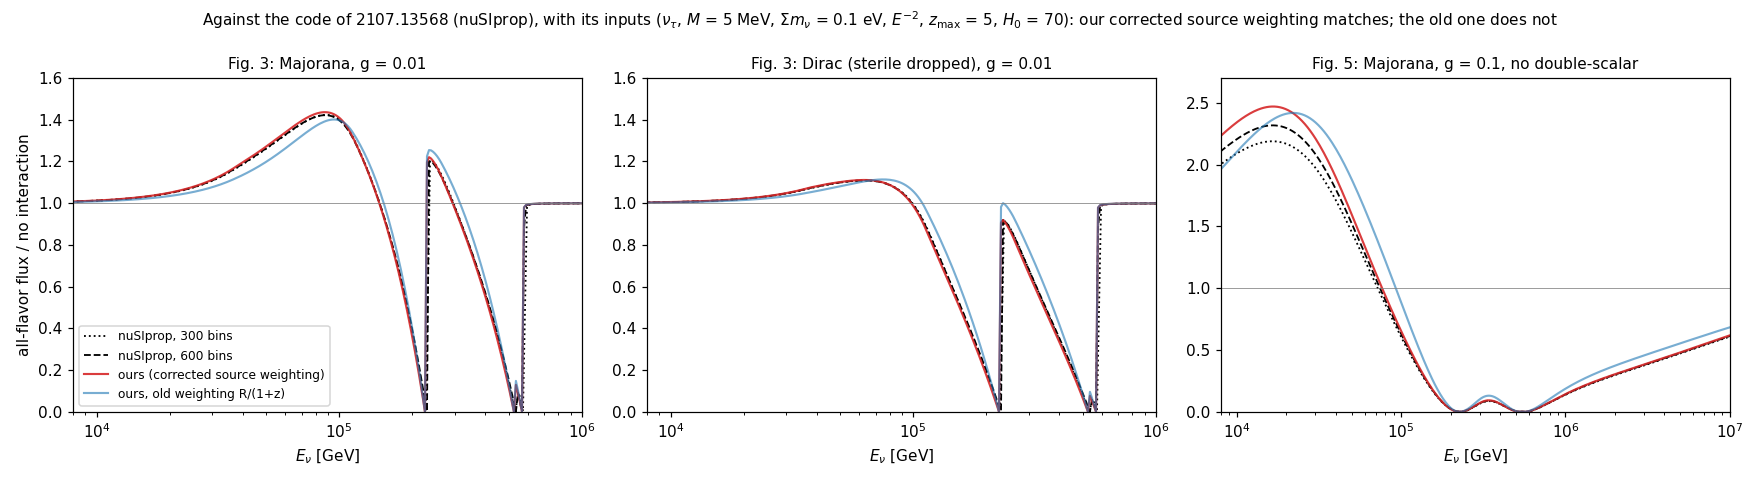
\includegraphics[width=\textwidth]{../output/figures/si_nusiprop_comparison.png}
\caption{\textbf{Against nuSIprop}, the code of 2107.13568, with its inputs: its Fig.~3 (Majorana and
Dirac, $g = 0.01$) and Fig.~5 ($g = 0.1$, without double-scalar production), nuSIprop at 300 and 600
bins against our transport with the corrected source weighting and with the old one.}
\label{fig:si_nusiprop}
\end{figure}

\textit{Effect.}---Without interactions the flux is a pure power law either way, and the flavor
composition does not depend on the weighting; with them, weight moves to higher redshift, where the
relic density, the cosmological potential and the resonance crossings differ. Every plane was
recomputed (Sec.~\ref{sec:si_models} and Sec.~\ref{sec:stats}); the secret-interaction limits became stronger by $\sim10\%$ (the median ratio of new to old per
mass column is $0.81$--$0.93$ across the 19 planes; best limits, e.g., $\nu_e$ $1.7\to1.5\times10^{-5}$,
universal $8.8\to8.0\times10^{-6}$), with single columns near the window's allowed channels moving
by large factors either way; the dark portal's potential planes and its exclusion plane are unchanged
in the median (single columns up to a factor 2), its MeV planes $3$--$23\%$ stronger.
\file{output/analysis/} (Tycho jobs 66307194--99, commit \texttt{124fd03}).

\subsection{The Galactic gas at $N_{\rm side} = 64$ (2026-10-14)}

The first track rates (Section~\ref{sec:dr2}) showed no Galactic flux for the dark portal and standard physics,
while the secret-interaction case, whose Galactic flux needs no emission points, had it. The gas columns of the
emission model (Söding et al.) come natively at $N_{\rm side} = 64$ in Galactic coordinates; the reduction
averaged the native pixels whose centres fall in each equatorial pixel, which at the same resolution, rotated,
leaves 12\% of the pixels with none: $0/0$. The check that every line of sight carries emission tested
${\rm total} \le 0$, which NaN passes, and the emission populations then dropped every density node such a
pixel touched, leaving 17 of 49\,152 pixels with Galactic flux. Fixed: as fine as the native maps, the reduction
interpolates the native columns at each pixel's centre (bilinear on the sphere); coarser (the committed
$N_{\rm side} = 16$, unchanged bit for bit), it averages as before. Both checks now reject non-finite values
(\file{tests/test\_galactic.py}). The flavor fits, at $N_{\rm side} = 8$ from the $N_{\rm side} = 16$ data, were
never affected.

\subsection{The mixing-parameter priors (found 2026-10-12)}
\label{app:priors}

The Gaussian priors in the \texttt{fallbacks} block of the analysis configurations have never
been applied, for three reasons. First, the configurations name the shape \texttt{"gaussian"}, while
the code accepts only \texttt{"gauss"}. Second, the entries \texttt{dcp} and \texttt{dm3l\_sq}
do not match the parameter names \texttt{d\_cp\_deg} and \texttt{dm31\_sq}. Third, the prior
centres disagree with the fixed values ($\delta_{\rm CP}$ $212^\circ$ against $132^\circ$,
$\Delta m^2_{21}$ $7.537\times10^{-5}$ against $7.41\times10^{-5}$~eV$^2$, which is $3.4\sigma$
of the prior). In addition, the branch for angles in degrees converts a value that is already
in degrees. The NuFIT~6.1 constraints of Sec.~\ref{sec:syst} will replace these priors.
FrequentistAnalysis was retired on 2026-10-12; the analysis package that replaced it applies its
priors and checks their names against the model's parameters (Sec.~\ref{sec:stats}).

\subsection{Earlier corrections}

\textit{Thermal kernel (July 2026).}---The midpoint-rule momentum integral erred by 6--9\% at
on-resonance cells; validation against the previous code could not reveal this, since it
measures only differences. A dense reference integration did. The semi-analytic kernel
replaced it, which changed the fluxes at the dips by up to 15\% with flavor ratios within
$10^{-6}$ and dip energies unchanged (round 7).

\textit{Earth steps (July 2026).}---The left-endpoint stepping scattered the results at the
$10^{-2}$ level under any change of the step count (Sec.~\ref{sec:earth}); in-band
energy-averaged flavor ratios carried a $1.7\times10^{-2}$ ambiguity at the analysis settings.
The phase-exact scheme removed it.

\textit{Coupling cache (July 2026).}---The cache never activated in real scans
(Sec.~\ref{sec:thermal}); its narrower brackets fixed that without loss of accuracy.

\end{document}
